\documentclass[xcolor=dvipsnames]{beamer}
\usepackage{pgf}
\usepackage{tikz}
\usepackage{amsmath,amssymb}
\usepackage{pifont}
\usepackage[latin1]{inputenc}
\usepackage{colortbl}
\usepackage[english]{babel}
\usepackage{comment}
\usepackage{soul}
\usepackage{xspace}
\usepackage{hyperref}
\usepackage{booktabs}        % professional-quality tables
\usepackage{multirow}
\usepackage{standalone}

\usepackage{grffile}
\usepackage{upgreek}
\newcommand{\bmmax}{0} % to fix bold greek fonts
\usepackage{bm}
\usepackage[noend,noline,ruled]{algorithm2e}
\include{mathmacro}


\usetikzlibrary{backgrounds}
\usetikzlibrary{arrows,shapes}
\usetikzlibrary{automata}
\usetikzlibrary{positioning}
\usetikzlibrary{decorations.pathmorphing}
\usetikzlibrary{intersections}
\usetikzlibrary{calc}
\usetikzlibrary{fit}
\usepackage[skins]{tcolorbox}

\usepackage[framemethod=default]{mdframed}


\makeatletter
\newcommand{\bfgreek}[1]{\bm{\@nameuse{#1}}}
\makeatother


\setbeamercovered{invisible}

\usetheme{Malmoe}
\useoutertheme{infolines}
\usefonttheme[onlymath]{serif}
\setbeamertemplate{footline}{%
    \begin{beamercolorbox}[wd=\paperwidth,ht=2.25ex,dp=1ex,right,
      rightskip=4mm, leftskip=5mm]{section in head/foot}
        \inserttitle\hfill\insertauthor\hfill\insertframenumber%
    \end{beamercolorbox}
}
%\setbeamertemplate{footline}[text line]{Greg
%  Shakhnarovich,~~~~Segmentation/cascades,~~~\insertframenumber / \inserttotalframenumber}
\setbeamertemplate{itemize item}[ball]
\setbeamertemplate{itemize subitem}[circle]
\setbeamertemplate{enumerate item}[square]
\setbeamerfont{itemize/enumerate subbody}{size=\normalsize}
\setbeamertemplate{navigation symbols}[only frame symbol]
\setbeamertemplate{subsection in toc shaded}[default][60]

\setbeamertemplate{frametitle}
{
\begin{centering}
\color{black}
\textbf{\insertframetitle}
\par
\end{centering}
}
\setbeamercolor{normal text}{fg=blue!50!black}
\setbeamercolor{math text}{fg=black}
%\setbeamercolor{math text inlined}{use={normal text},fg=normal text.fg}
\setbeamercolor{normal text in math text}{use={normal text},fg=normal text.fg}

\setbeamercolor{bibliography item}{fg=Green}

\usetikzlibrary{shapes,calc,positioning,patterns,decorations.pathmorphing}



\tikzset{cnode/.style={circle,draw,thick,minimum size=2em,inner sep=0pt}}

\tikzset{cnodesmall/.style={circle,draw,thick,minimum size=.5em}}

\colorlet{ffcol}{green!60!black}
\colorlet{bpcol}{red!60!black}



\definecolor{mycolor}{rgb}{0.622, 0.535, 0.698}
\definecolor{superlightgray}{rgb}{0.95, 0.95, 0.93}

\newmdenv[innerlinewidth=4.5pt, roundcorner=24pt,linecolor=mycolor,innerleftmargin=6pt,
innerrightmargin=6pt,innertopmargin=6pt,innerbottommargin=6pt]{linkbox}

\newmdenv[innerlinewidth=0, roundcorner=4pt,backgroundcolor=lightgray,linecolor=mycolor,innerleftmargin=7pt,
innerrightmargin=7pt,innertopmargin=7pt,innerbottommargin=7pt]{codebox}

\newmdenv[innerlinewidth=5pt, roundcorner=4pt,backgroundcolor=superlightgray,linecolor=mycolor,innerleftmargin=5pt,
innerrightmargin=5pt,innertopmargin=5pt,innerbottommargin=5pt]{relatedbox}

\DeclareMathAlphabet{\mathbfsf}{\encodingdefault}{\sfdefault}{bx}{n}


\newcommand{\gt}[1]{col-examples/ctest10k-supp/gt/#1}
\newcommand{\gs}[1]{col-examples/ctest10k-supp/grayscale/#1}
\newcommand{\mm}[1]{col-examples/ctest10k-supp/output/#1}

\newcommand{\cmark}{\ding{51}}
\newcommand{\xmark}{\ding{55}}

\newcommand{\cmt}[1]{\iffalse #1 \fi}
\def\dash{-\phantom{.0}}
\def\ndash{-}
\def\amp{\&} % doesn't screw up table formatting

\def\preli{}
\def\rough{}
\def\guess{}

\def\etal{\emph{et al.}}


\definecolor{cadmiumgreen}{rgb}{0.0, 0.42, 0.24}
\definecolor{deepmagenta}{rgb}{0.8, 0.0, 0.8}
\definecolor{goldenrod}{rgb}{0.85, 0.65, 0.13}

\definecolor{darkgreen}{rgb}{0.0, 0.80, 0.24}


\newcommand{\mycite}[1]{\textcolor{Green}{[{#1}]}}

% TODO: make this directly reference normal text color
\newcommand{\myar}{$\textcolor{blue!50!black}{\Rightarrow}$}

%\date{October 22, 2010}

\colorlet{ffcol}{green!60!black}
\colorlet{bpcol}{red!60!black}


\newcommand{\convarr}[3][ffcol]{% 
% 1: color (default ffcol)
% 2: node label(name)
% 3: distance from node in y
  \foreach \xs in {-.5cm,-.3cm,.5cm} {%
    \draw[{#1},thick,-latex] let \p1 = (#2) in %
    ($ (\x1,\y1)+(\xs,{#3}) $) -- (#2);%
  }%
  \draw let \p1 = (#2) in node at ($ (\x1,\y1)+(0,{#3}) $) {\tiny $\textcolor{#1}{\ldots}$};%
}%

\newcommand{\divarr}[3][ffcol]{% 
% 1: color (default ffcol)
% 2: node label(name)
% 3: distance from node in y
  \foreach \xs in {-.5cm,-.3cm,.5cm} {%
    \draw[{#1},thick,-latex] let \p1 = (#2) in %
    (#2) -- ($ (\x1,\y1)+(\xs,{#3}) $) ;%
  }%
  \draw let \p1 = (#2) in node at ($ (\x1,\y1)+(0,{#3}) $) {\tiny $\textcolor{#1}{\ldots}$};%
}%


\title{Deep Learning Tutorial\\Part II}

\institute{%
  \vspace{-1em}\begin{minipage}[t]{.25\linewidth}%
    \vspace{-3em}%
    \includegraphics[width=.8in]{tticlogo}\vspace{2em}%
  \end{minipage}%
  \begin{minipage}[t]{.5\linewidth}%
    {\Large Greg Shakhnarovich}\\{\Large TTI-Chicago\vspace{2em}}%
  \end{minipage}%
}



\date{December 2016}

\begin{document}

\maketitle

\section{Overview}

\begin{frame}
  \frametitle{Goals of the tutorial}
\bi
\item Somewhat organized overview of basics, and some more advanced
  topics
\item Demistify jargon
\item Pointers for informed further learning
\item Aimed mostly at vision practitioners, but tools are widely
  applicable beyond vision
\item Assumes basic familiarity with machine learning
\ei  
\end{frame}

\begin{frame}
  \frametitle{Not covered}
  \bi
\item Connections to brain
\item Deep learning outside of neural networks
\item Many recent advances
\item Many specialized architectures for vision tasks
\ei
\end{frame}


\begin{frame}
  \frametitle{Outline}
Introduction (3 hours):
\bi
\item Review of relevant machine learning concepts
\item Feedforward neural networks and backpropagation
\item Optimization techniques and issues
\item Complexity and regularization in neural networks
\item Intro to convolutional networks
\ei
Advanced (3 hours):
\bi
\item Advanced techniques for learning DNNs
\item Very deep networks
\item Convnets for tasks beyond image classification
\item Recurrent networks
\ei
\end{frame}

\begin{frame}
  \frametitle{Sources}
  \bi
\item Stanford CS231N: Convolutional Neural Networks for Visual
  Recognition\\
Andrej Karpathy, Justin Johnson et al. (2016 edition)\\
\url{vision.stanford.edu/teaching/cs231n}
\item Deep Learning by Ian Goodfellow, Aaron Courville and Yoshua
  Bengio, 2016
\item Chris Olah: Understanding LSTM Networks (blog post)\\
\url{colah.github.io/posts/2015-08-Understanding-LSTMs}
\item Papers on arXiv and slides by the authors
\ei
\end{frame}

\section{More training tricks}

\begin{frame}
  \frametitle{Input normalization}
  \bi
\item Standard practice: normalize the data
\item Theoretically could apply a variety of normalization schemes:\\
zero-mean\\
unit variance\\
``box normalization''\\
whitening
\item In practice, for images: subtract ``mean pixel'' (same for all
  locations)
\item Assuming zero-mean filters: zero-mean filter response
\item Matches zero padding
\ei
\end{frame}

\begin{frame}
  \frametitle{Batch normalization: motivation}
  \bi
\item Problem: covariance shift (change in function's domain)
\item As learning proceeds, higher layer suffer from \emph{internal}
  covariance shift due to changing parameters of previous layers
\item Makes learning harder!
\item Example: MNIST (15/50/85 percentile of input to typical sigmoid)
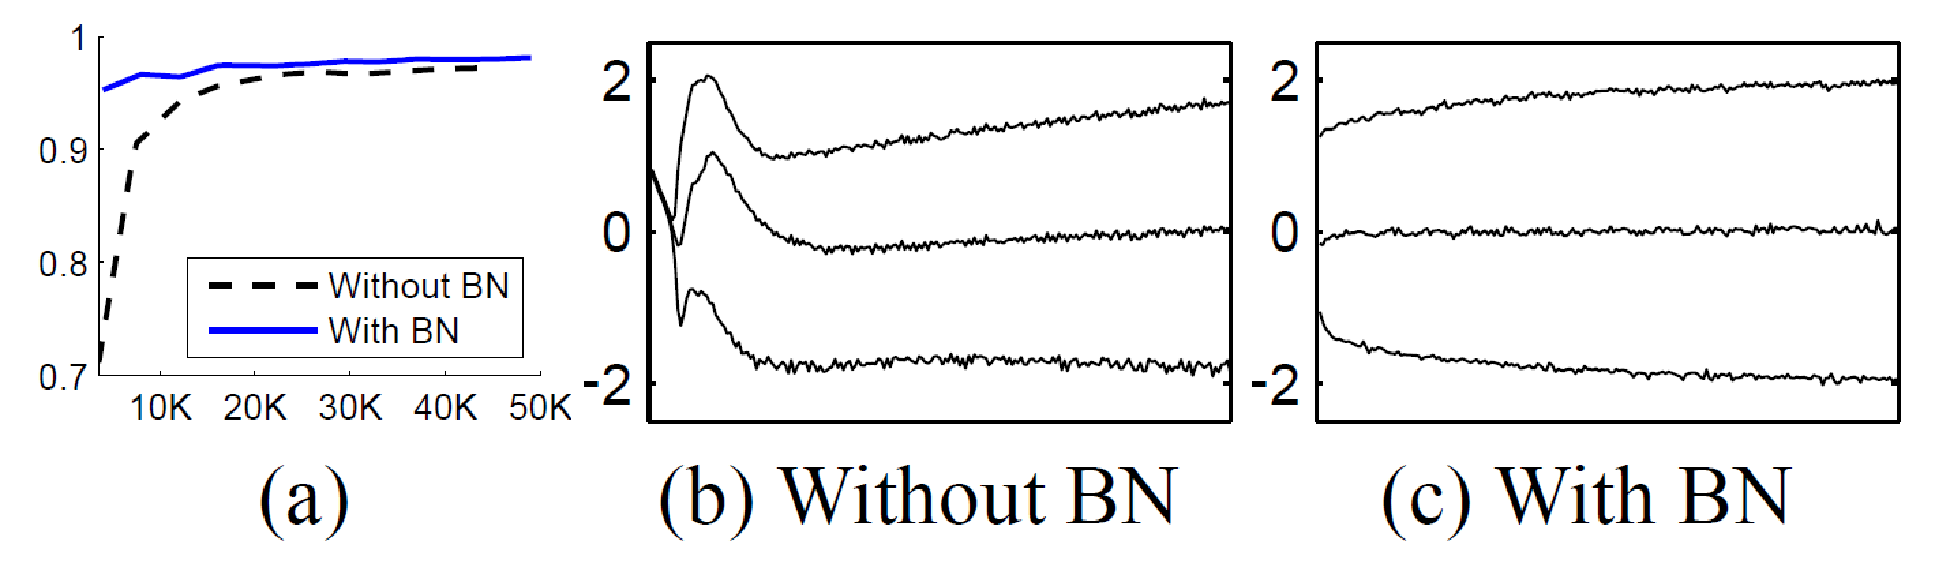
\includegraphics[width=.8\textwidth]{bn-mnist}\\
{[Ioffe and Szegedy]}
\ei

\end{frame}

\begin{frame}
  \frametitle{Batch normalization: algorithm}
\bi
\item Batch normalization [Ioffe and Szegedy, 2015]

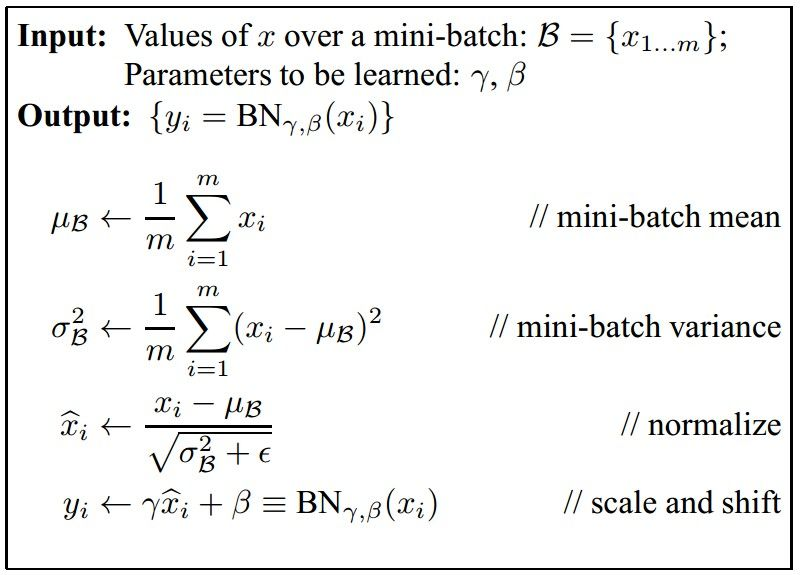
\includegraphics[width=.7\textwidth]{bn-algo}
\item Scale $\gamma$ and shift $\beta$ (per layer or psr channel) are
  learned through the usual backprop!
\ei
\end{frame}

\begin{frame}
  \frametitle{Batch normalization effect}
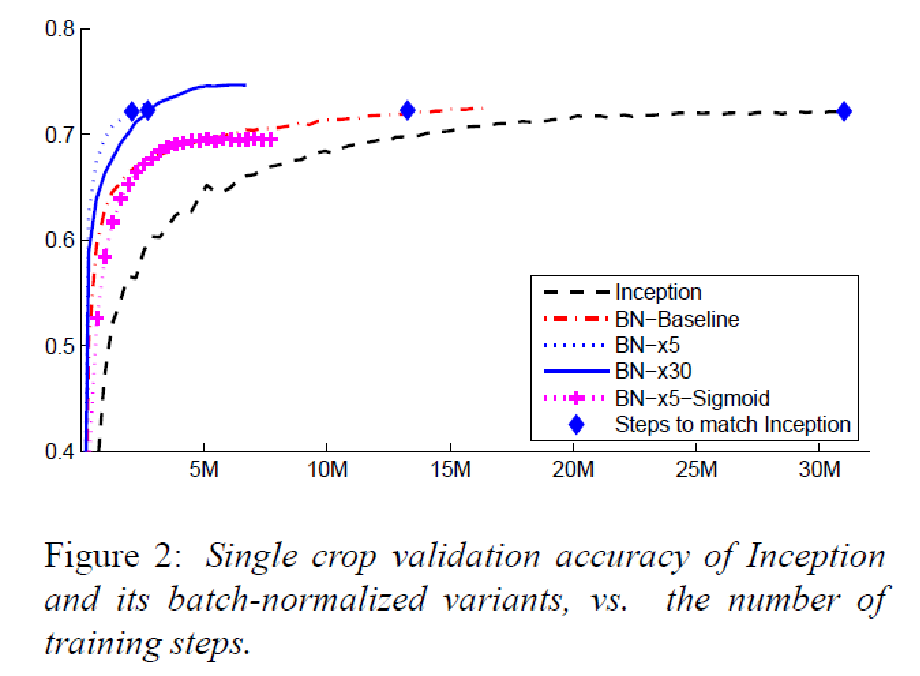
\includegraphics[width=.7\textwidth]{bn-inception}\raisebox{1em}{[Ioffe
  and Szegedy]}
  
\bi
\item Allows for higher learning rate, faster convergence
\item May (or may not) reduce need for dropout
\item De-factor standard today in most architectures
\ei

\end{frame}

\begin{frame}
  \frametitle{Data augmentation}
  \bi
\item Part of the invariances learned by convnets is due to including
  variations in the training set
\item Natural variation: different instances of objects, scene
  compositions etc.
\item Can get a lot more for free by synthetic variations
\item Obvious: mirror flip (horizontally -- but not vertically!)

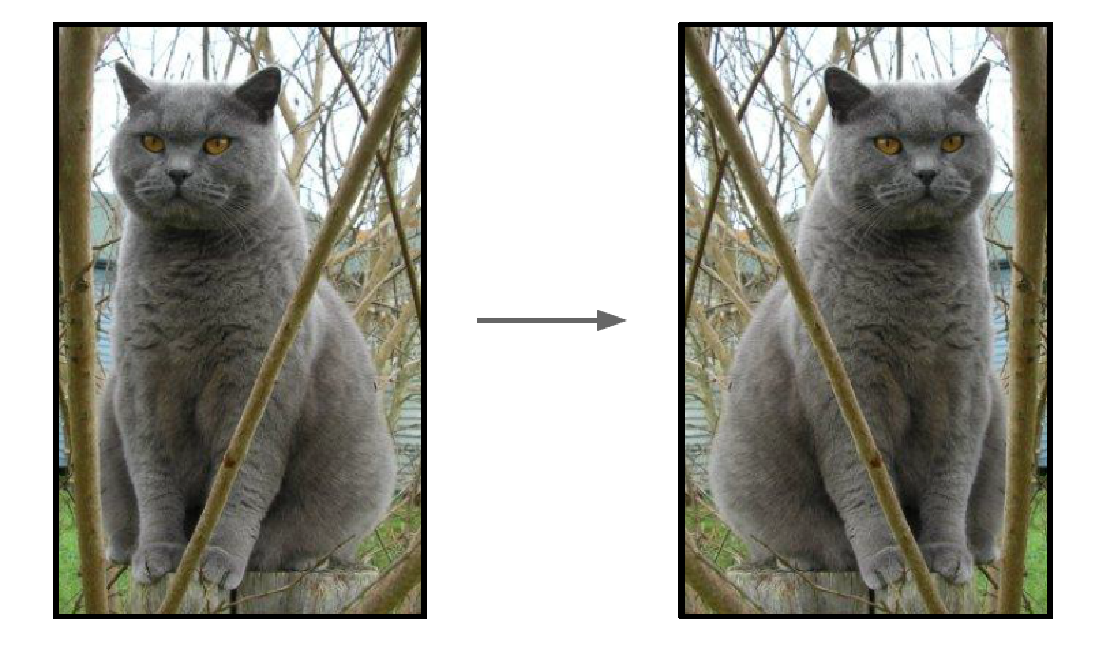
\includegraphics[width=.4\textwidth]{ak-mirror}\raisebox{1em}{[A. Karpathy]}

\ei
\end{frame}


\begin{frame}
  \frametitle{Data augmentation}
  \bi
\item Random crops (and scales)
\item For image classification -- assumes object is large and central
\ei
  \begin{minipage}[c]{.65\linewidth}
    \bi
\item E.g., training ResNet on ImageNet:\\
resize image so shorter size is a random number between 256 and 480;\\
crop random 224$\times$224 window
\ei
  \end{minipage}%
  \begin{minipage}[c]{.35\linewidth}
    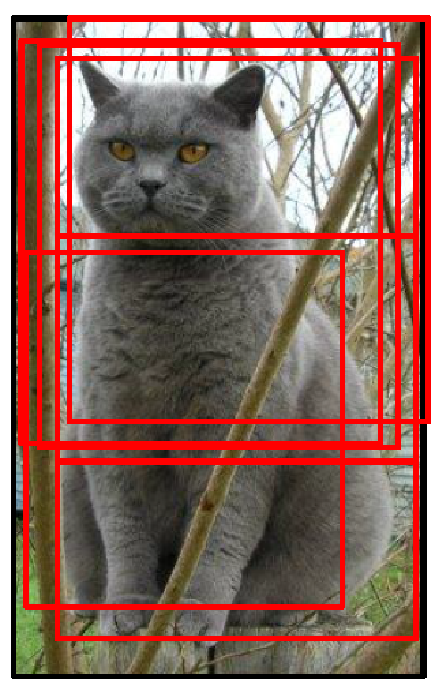
\includegraphics[width=.45\textwidth]{ak-crops-random}
    \uncover<2->{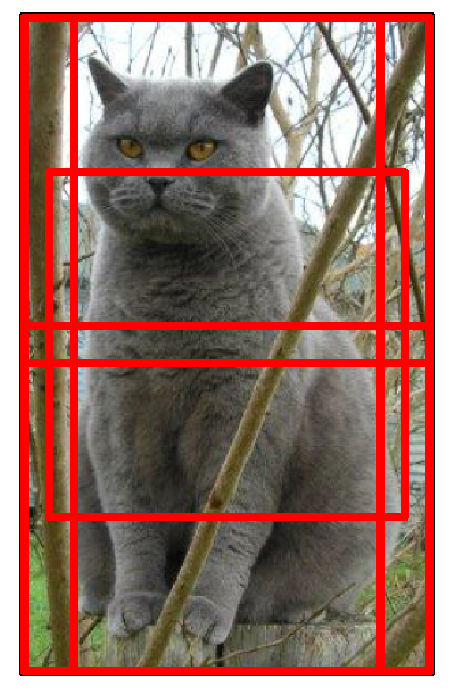
\includegraphics[width=.45\textwidth]{ak-crops}}
\\{[A. Karpathy]}

  \end{minipage}
\bi
\item Must match to testing regime\\
ResNet: multiple scales, fixed crops for each scale, max
\ei
\end{frame}


\begin{frame}
  \frametitle{Data augmentation}
  \bi
\item Color jitter
\ei
\begin{minipage}[c]{.6\linewidth}
  \bi
\item Apply in a structured way (e.g., using PCA on color) rather than
per-pixel
\ei
\end{minipage}%
\begin{minipage}[c]{.4\linewidth}
      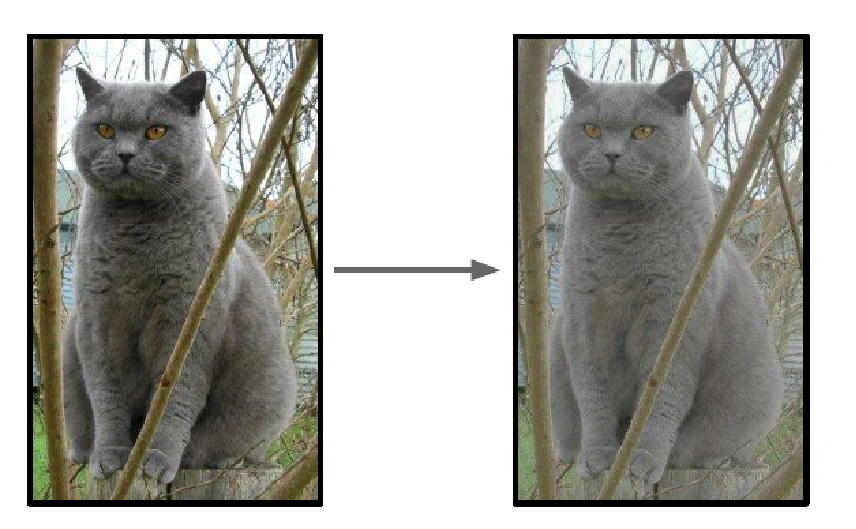
\includegraphics[width=.9\textwidth]{ak-colorjitter}\\{[A. Karpathy]}
\end{minipage}
\bi
\item Blur (see our paper on arXiv)
\item Rotations? Noise?
\ei
\end{frame}

\section{Very deep networks}

\begin{frame}
  \frametitle{Quest for very deep networks}
  \bi
\item Apparent dividends from depth (albeit diminishing):

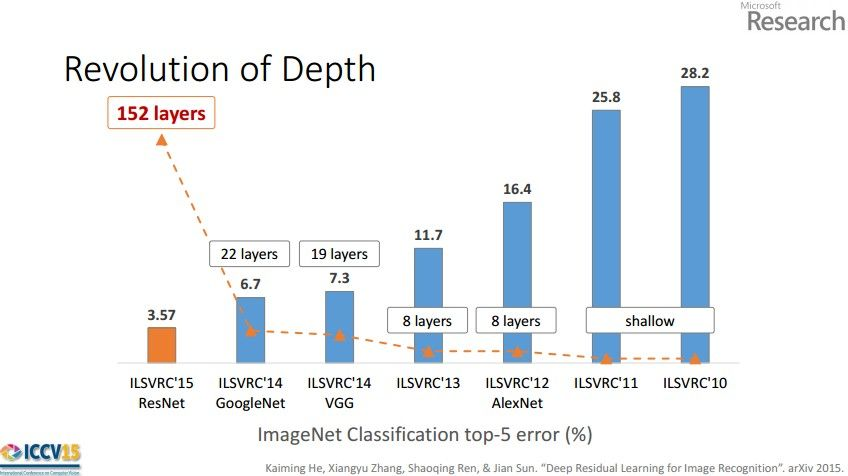
\includegraphics[width=.8\textwidth]{he-trend-slide}\\
{[He et al.]}
\item Three main challenges with depth:\\
computational complexity (alleviated by hardware?),\\
learning complexity; optimization complexity
\ei
\end{frame}

\begin{frame}
  \frametitle{Training very deep networks}
  \bi
\item Naive attempts to increase depth: CIFAR-10, simple sequence of
  $3\times3$ conv layers with occasional stride 2 (no pooling)

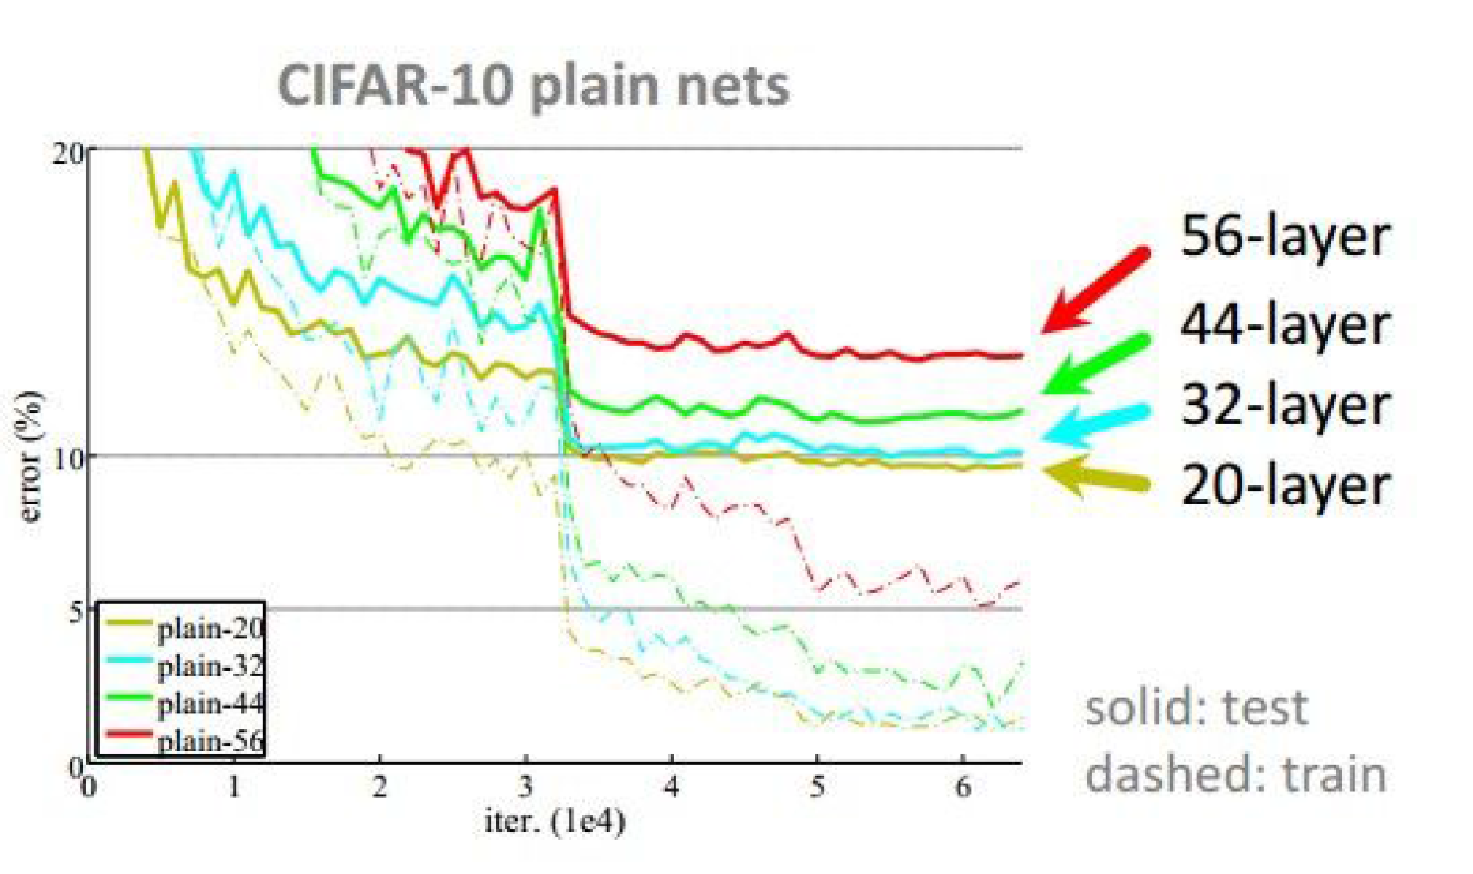
\includegraphics[width=.7\textwidth]{he-plaintrain}\\
{[He et al.]}
\item At certain depth optimization fails
\item Clearly an optimization issue (not learning)!
\ei
\end{frame}

\begin{frame}
  \frametitle{GoogleNet}
  \bi
\item A number of ad-hoc choices: ``inception blocks'', auxiliary loss
  paths
\item No fully connected layers!\\
compared to AlexNet: 12 times fewer parameters, double FLOPs
\ei

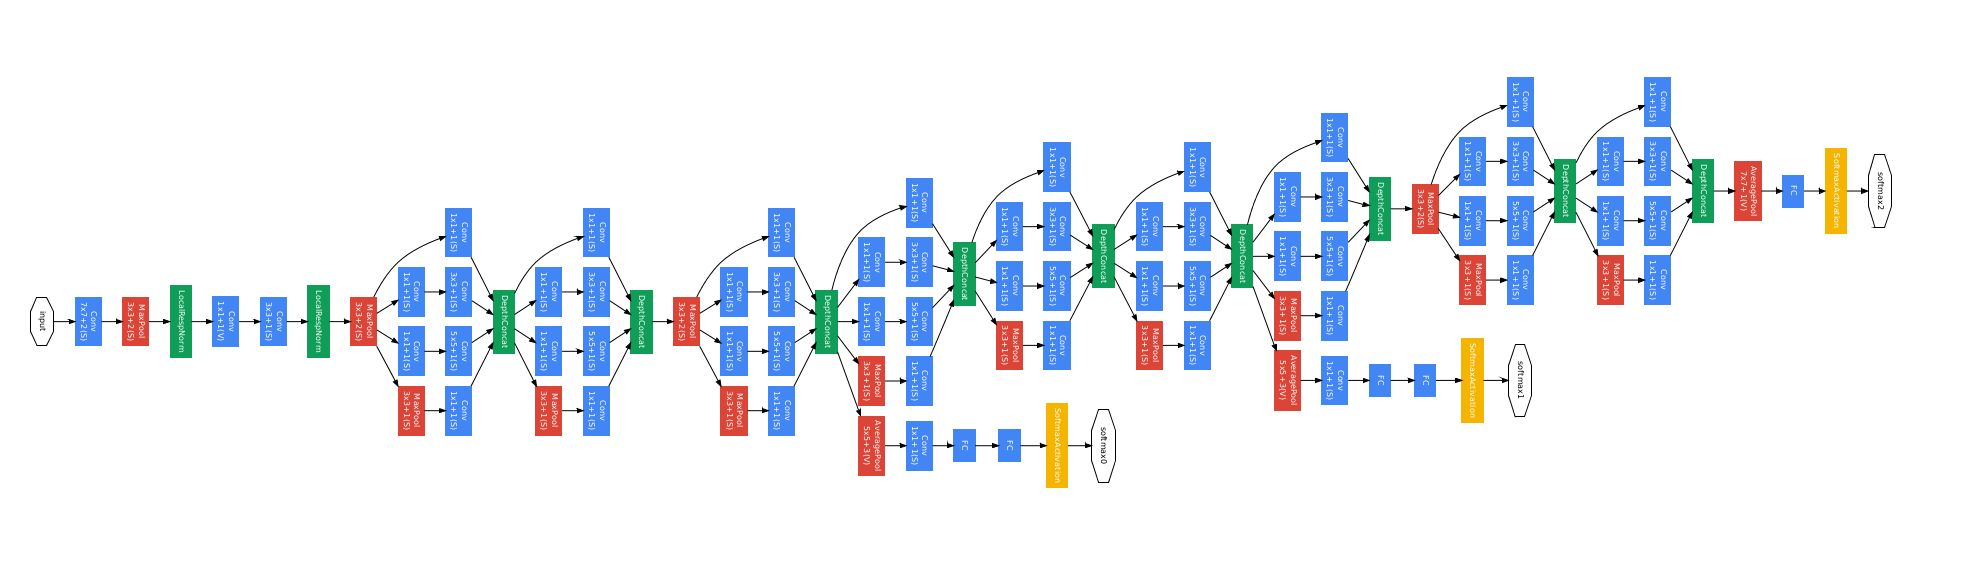
\includegraphics[width=.95\textwidth]{googlenet-2014}\\
{[Szegedy et al., 2014]}

\end{frame}

\begin{frame}
  \frametitle{Residual networks}
  \bi
\item Conventional wisdom: 
\item Key idea: allow for ``shortcuts'' for loss to reach low layers\\
``deep supervision''
\ei
\begin{minipage}[c]{.75\linewidth}
\bi

\item Residual connections [He et al., 2015]: learn what to add to the previous layer
  rather than how to modify it
\ei  
\end{minipage}%
\begin{minipage}[c]{.25\linewidth}
  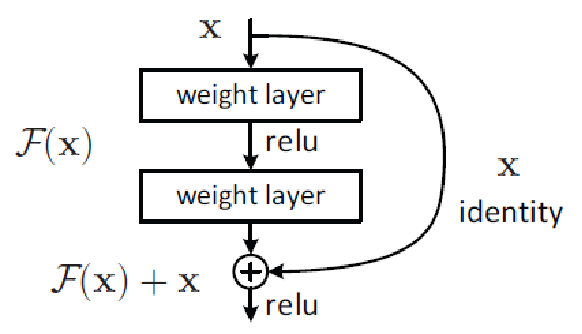
\includegraphics[width=.95\textwidth]{resnet-block}
\end{minipage}

\end{frame}


\begin{frame}
  \frametitle{ResNet architecture}
 
\bi
\item Compare to VGG-19 and to plain architecture
\ei
\hspace{-1em}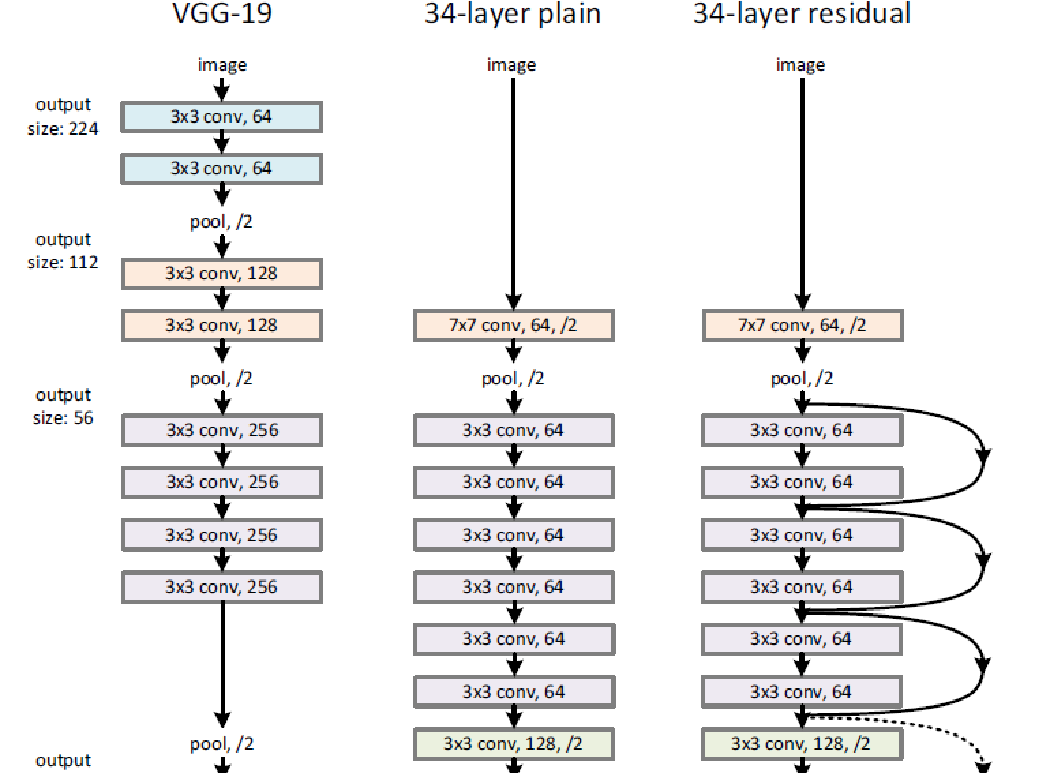
\includegraphics[width=.48\textwidth]{resnet-arch-top}\raisebox{5em}{\Large\bf \ldots}
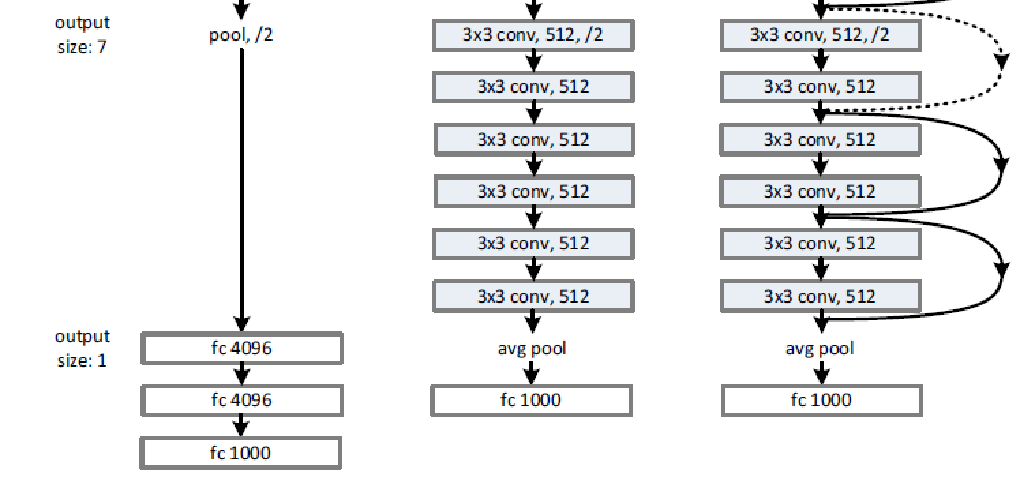
\includegraphics[width=.48\textwidth]{resnet-arch-bottom}

\end{frame}

\begin{frame}
  \frametitle{ResNet with bottleneck blocks}
   \begin{minipage}[c]{.75\linewidth}
  \bi
\item Bottleneck blocks:
\ei
  \end{minipage}%
  \begin{minipage}[c]{.25\linewidth}
      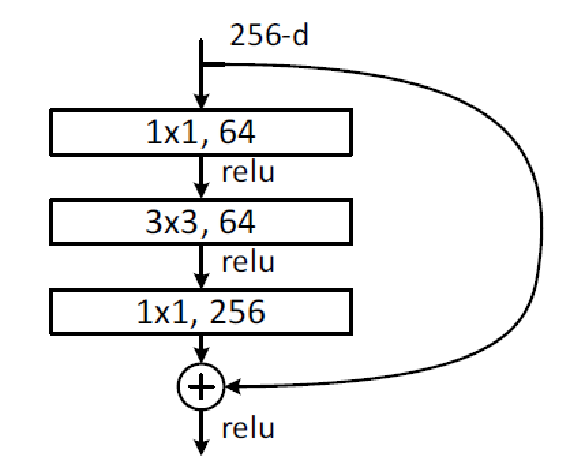
\includegraphics[width=.95\textwidth]{resnet-bottleneck-block}
  \end{minipage}
\bi
\item Can train hundreds of layers!\\
state of the art on ImageNet/COCO is ResNets with 150-250 layers
\item Similar to the Inception blocks in GoogleNet

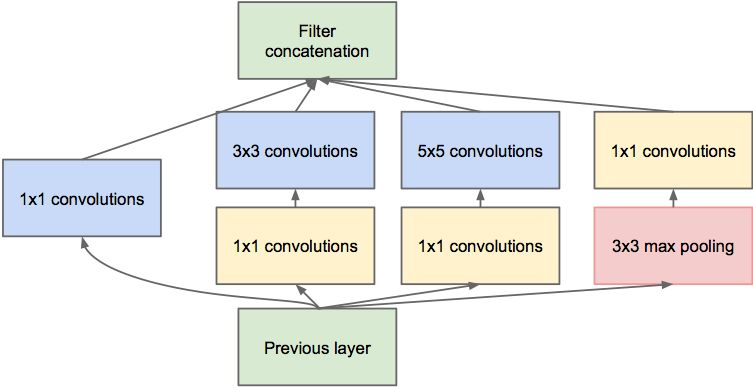
\includegraphics[width=.5\textwidth]{inception-block}

\ei
\end{frame}




\begin{frame}
  \frametitle{Stochastic depth}
  \bi
\item From dropping units to dropping layers: regularization by
  stochastic depth at train time!
\item Drop ``ResNet blocks'' with some probability
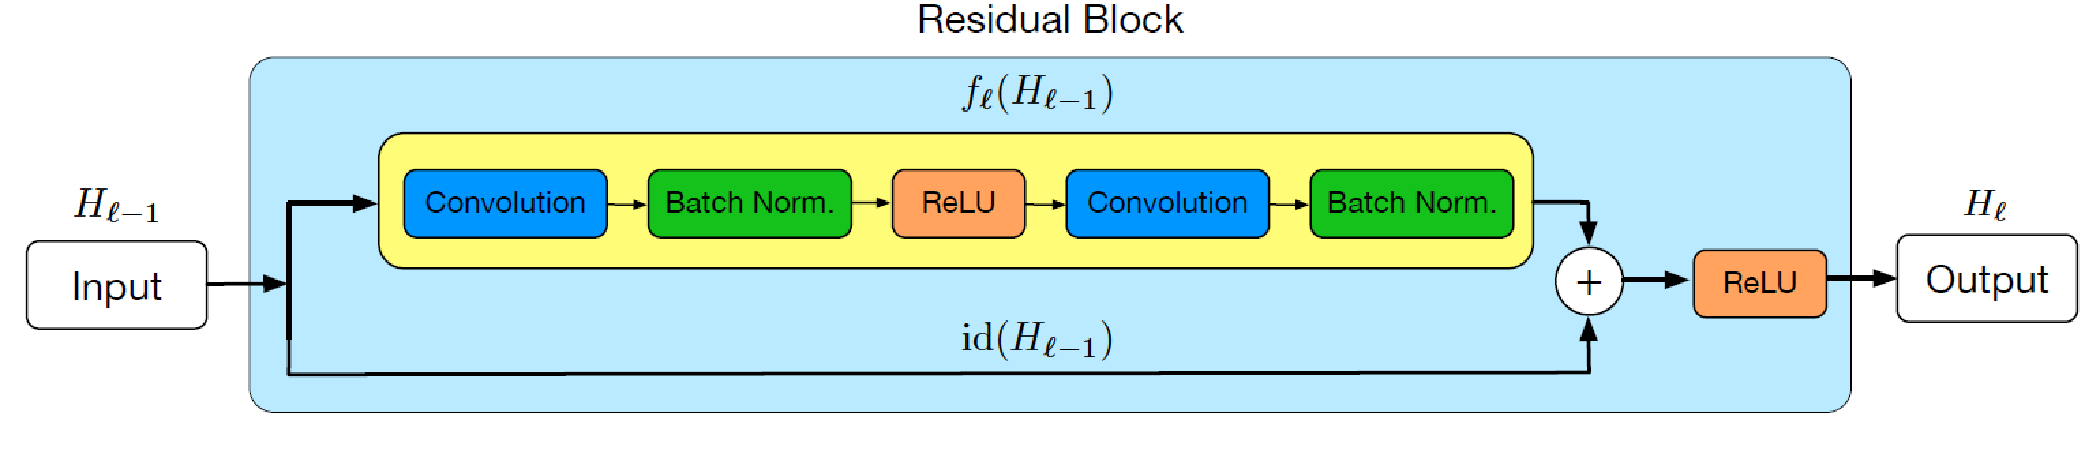
\includegraphics[width=.6\textwidth]{resblock}\\
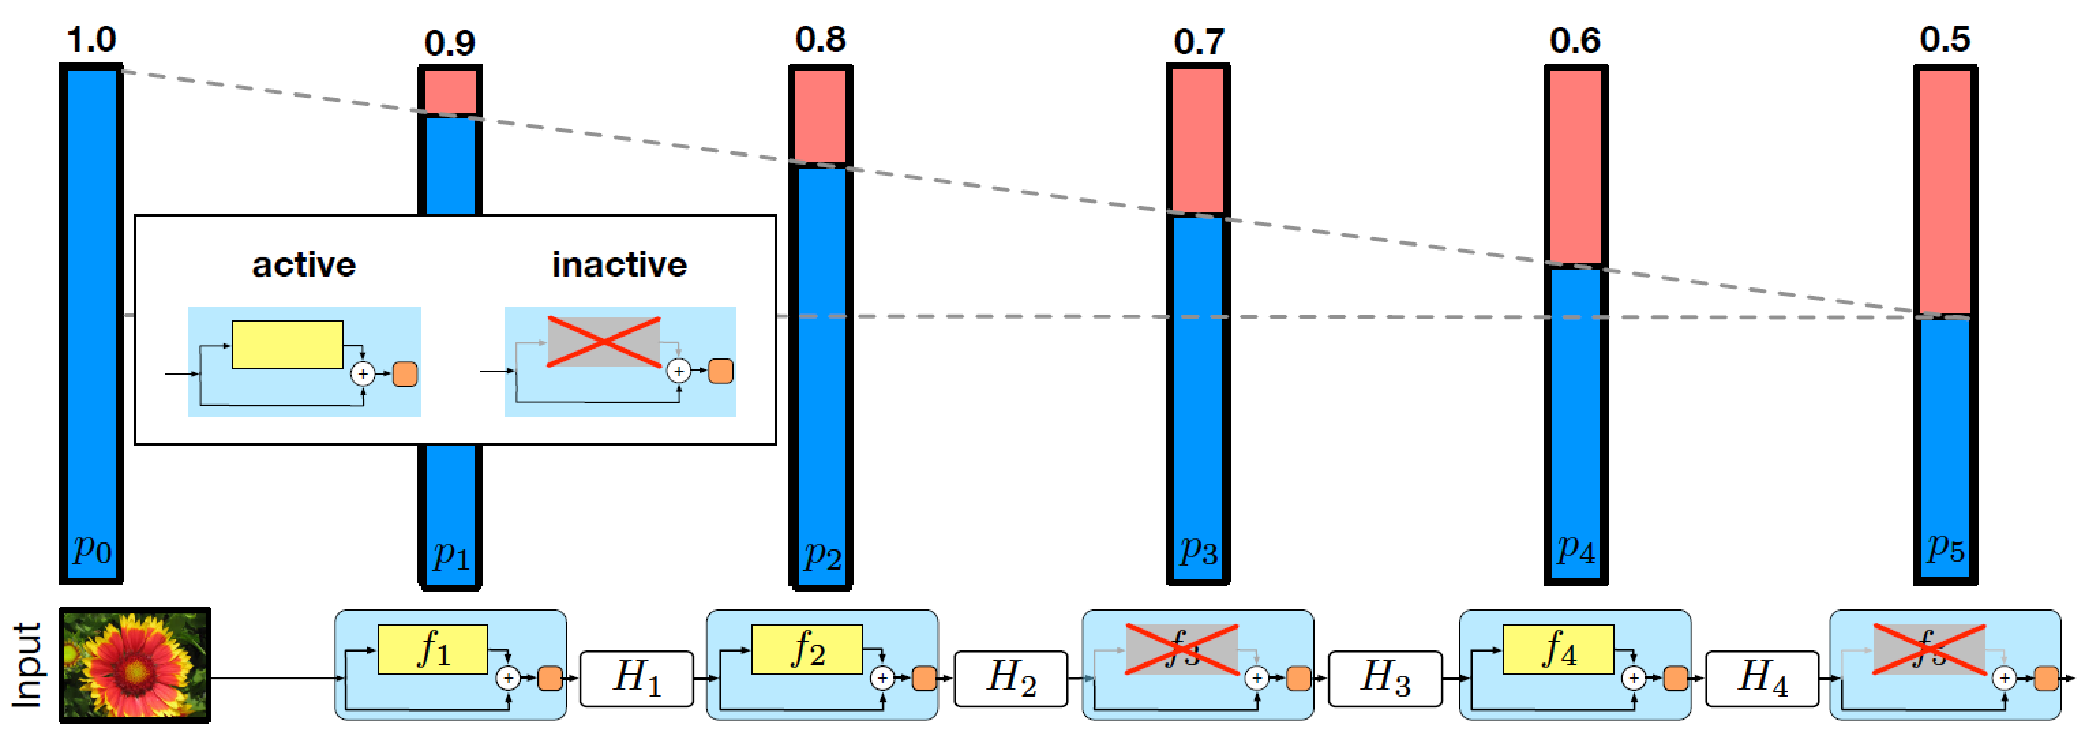
\includegraphics[width=.6\textwidth]{stoch-depth}\\
{[G. Hua et al., 2016]}
\item Made possible by the residual trick
\item State of the art on recognition tasks
\ei
\end{frame}






\section{Convnets for localization}

\begin{frame}
  \frametitle{Transfer learning with convnets}
  \bi\item Advice from Andrej Karpathy:
\ei

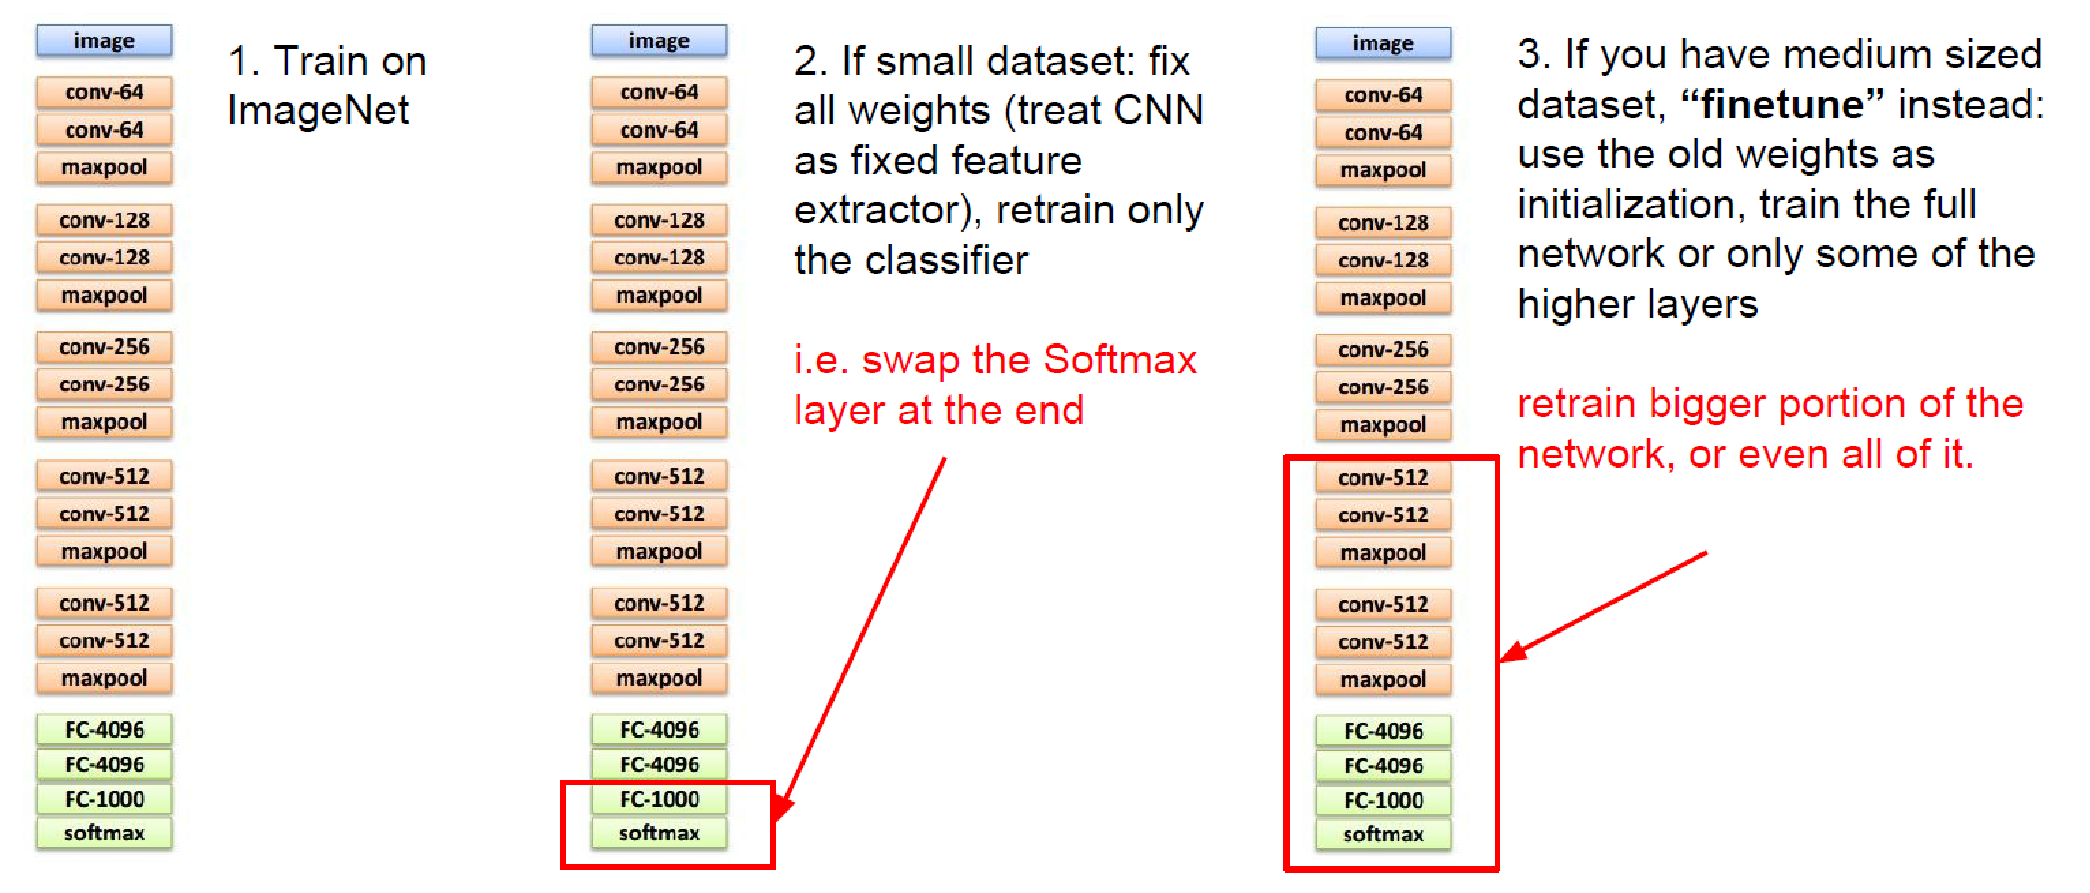
\includegraphics[width=.9\textwidth]{ak-transfer} 
\end{frame}


\begin{frame}
  \frametitle{Localization with convnets}
  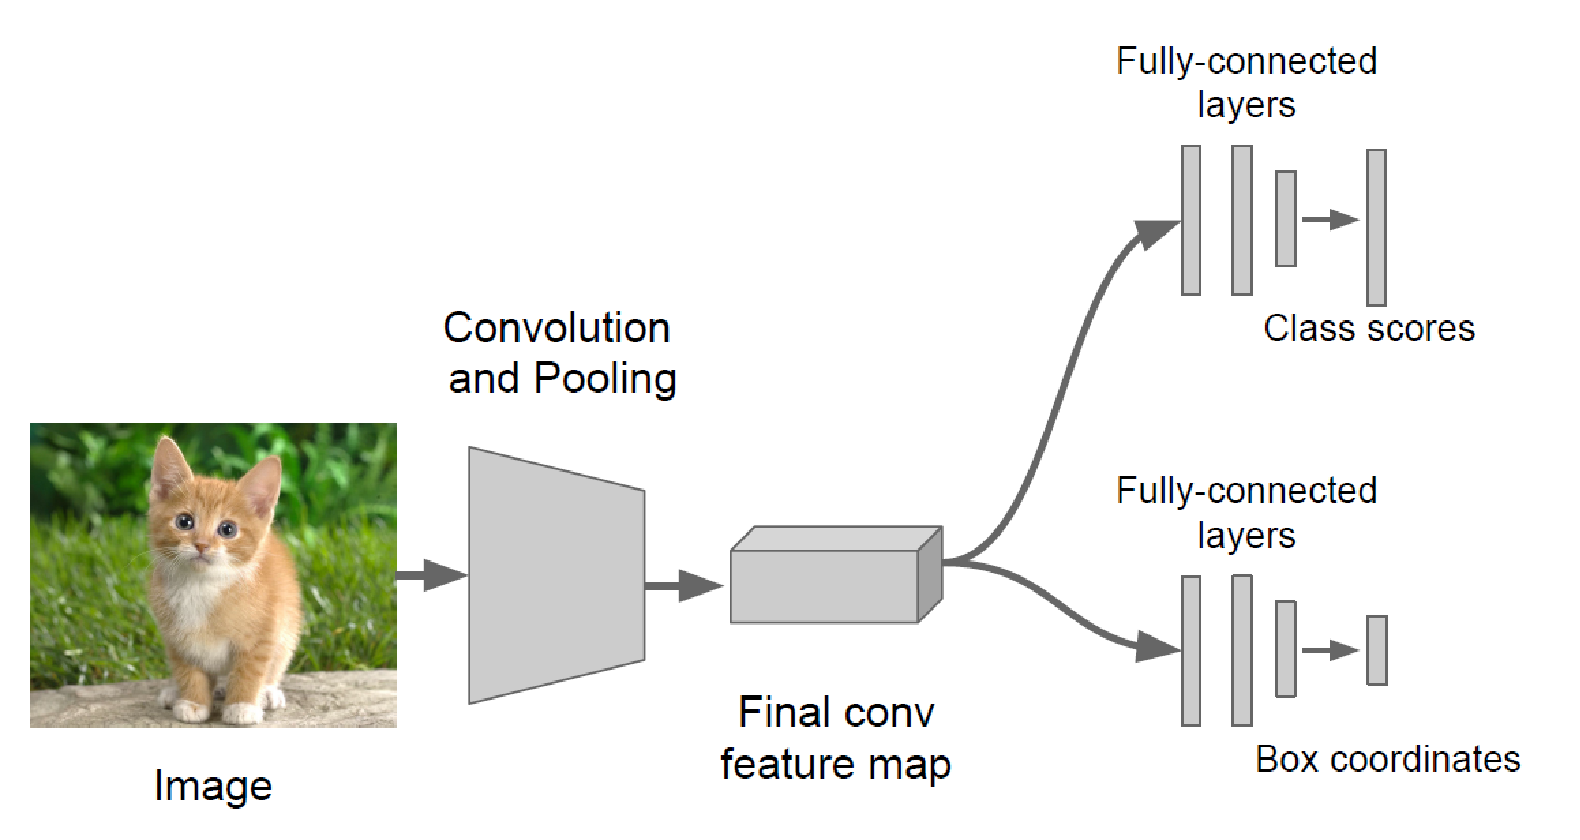
\includegraphics[width=.8\textwidth]{ak-localization-net}\raisebox{1em}{[A. Karpathy]}
\bi
\item Take classification net; discard top (fully connected) layers
\item Attach new sub-net for bounding box regression; train
\item At test time: use both classification and regression
\ei
\end{frame}

\begin{frame}
  \frametitle{Overfeat for detection}
\bi
\item Idea: reuse computation across overlapping sliding windows
\item Key innovation: convert ``fully connected'' to
  convolutional layers
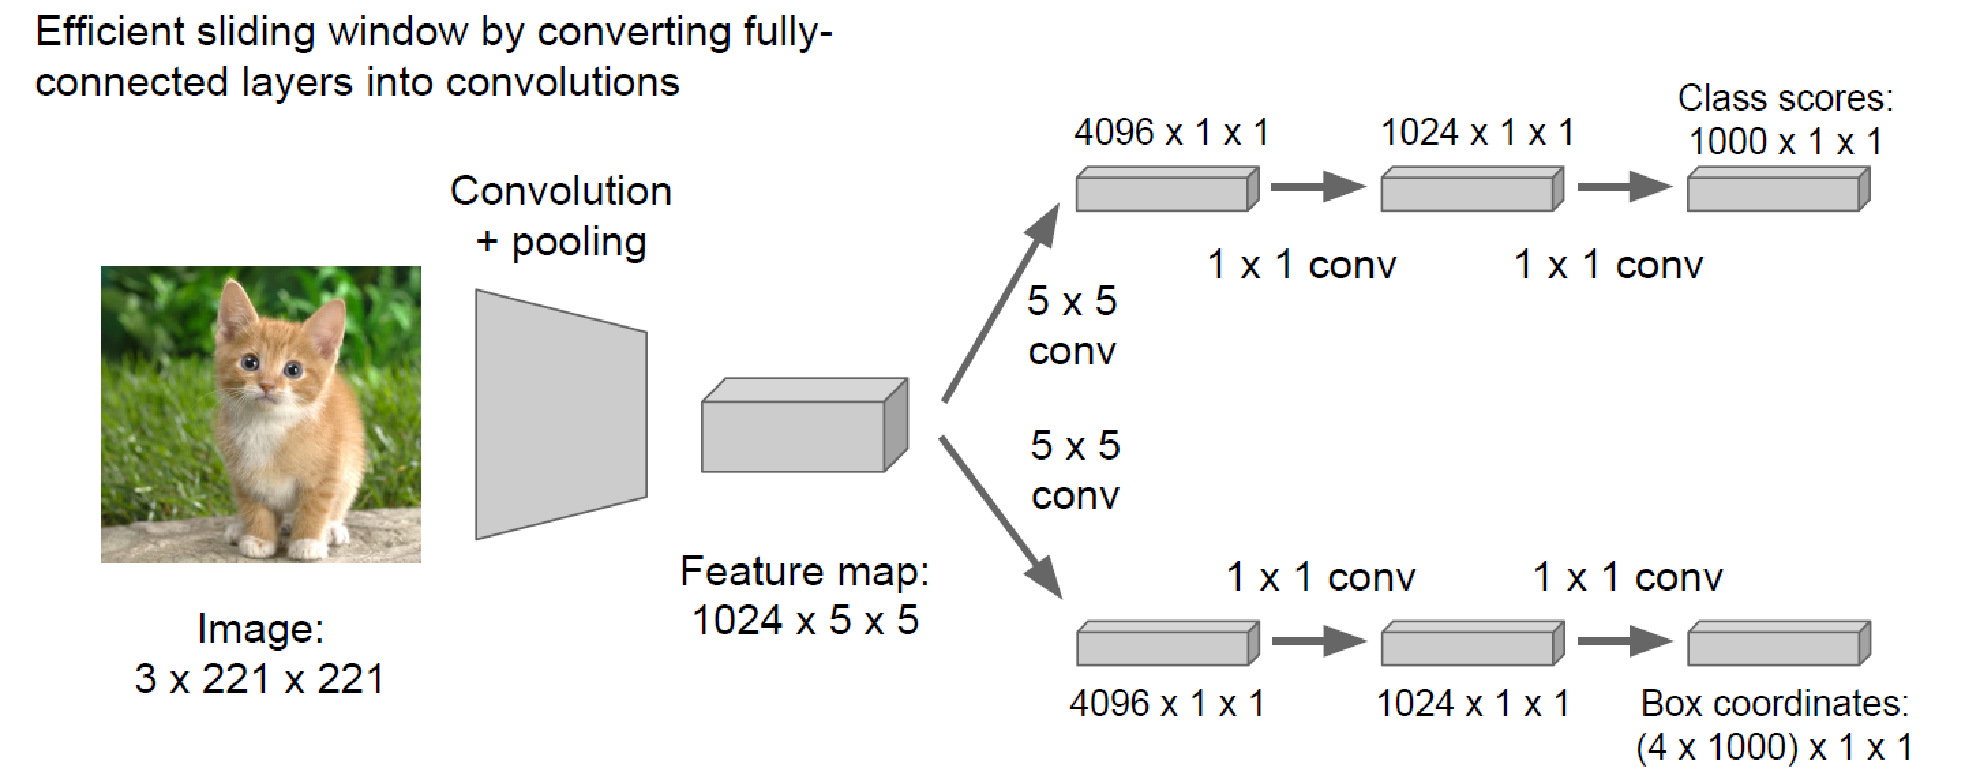
\includegraphics[width=.8\textwidth]{ak-overfeat-fc}\\
{[Sermanet et al.]}
\ei
\end{frame}

\begin{frame}
  \frametitle{Fully convolutional networks}
  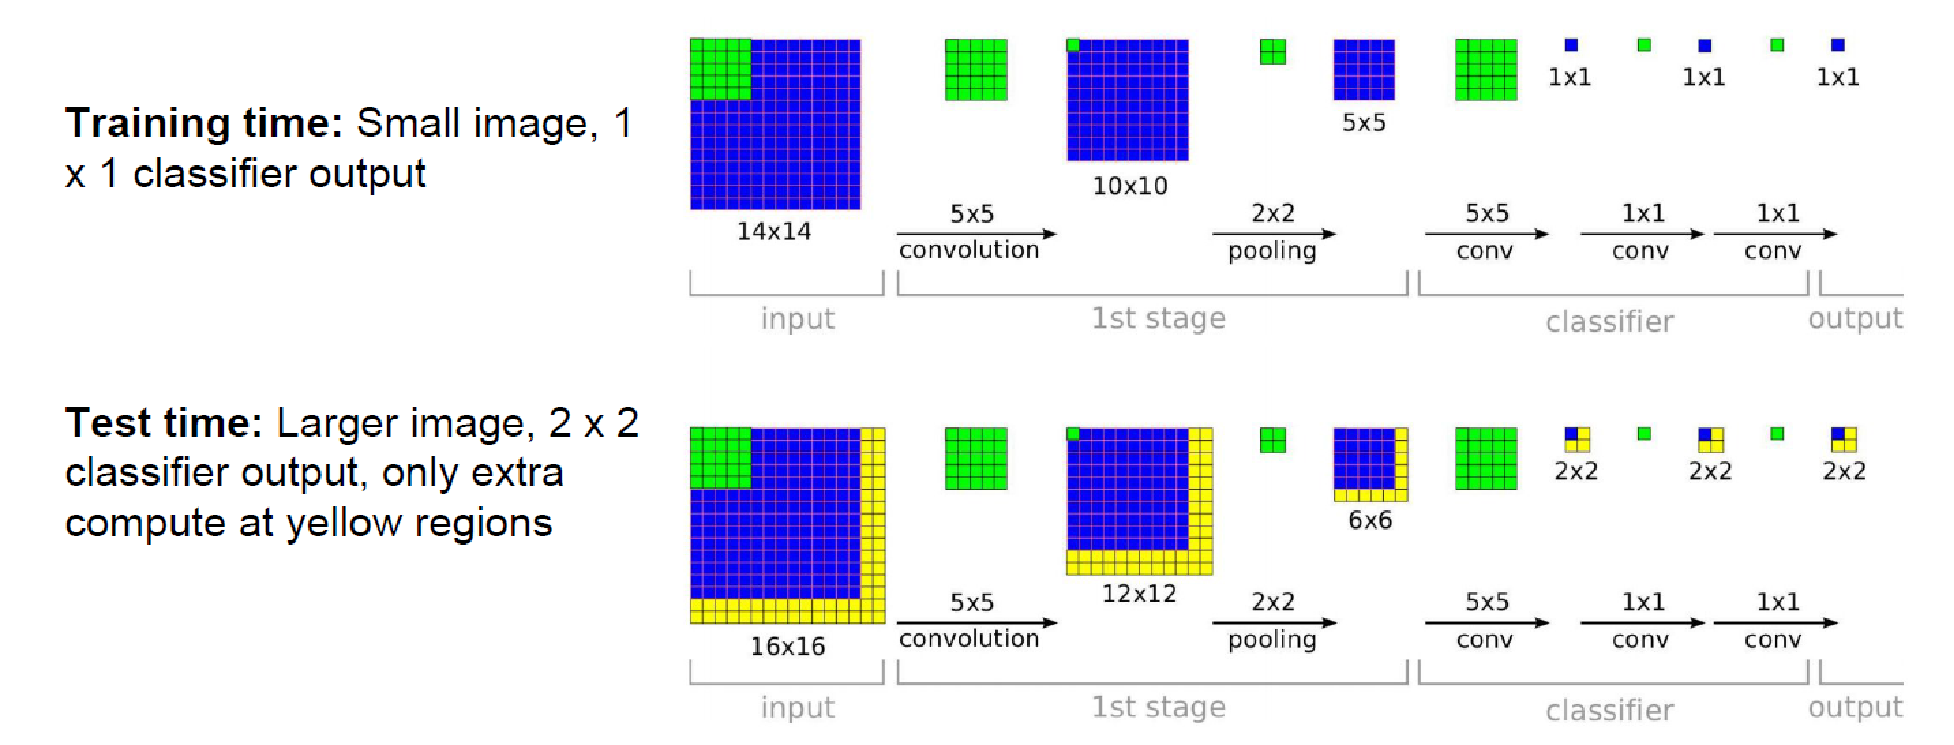
\includegraphics[width=.95\textwidth]{ak-overfeat-computation}\\
Overfeat [Sermanet et al.]
\end{frame}


\begin{frame}
  \frametitle{R-CNN}
  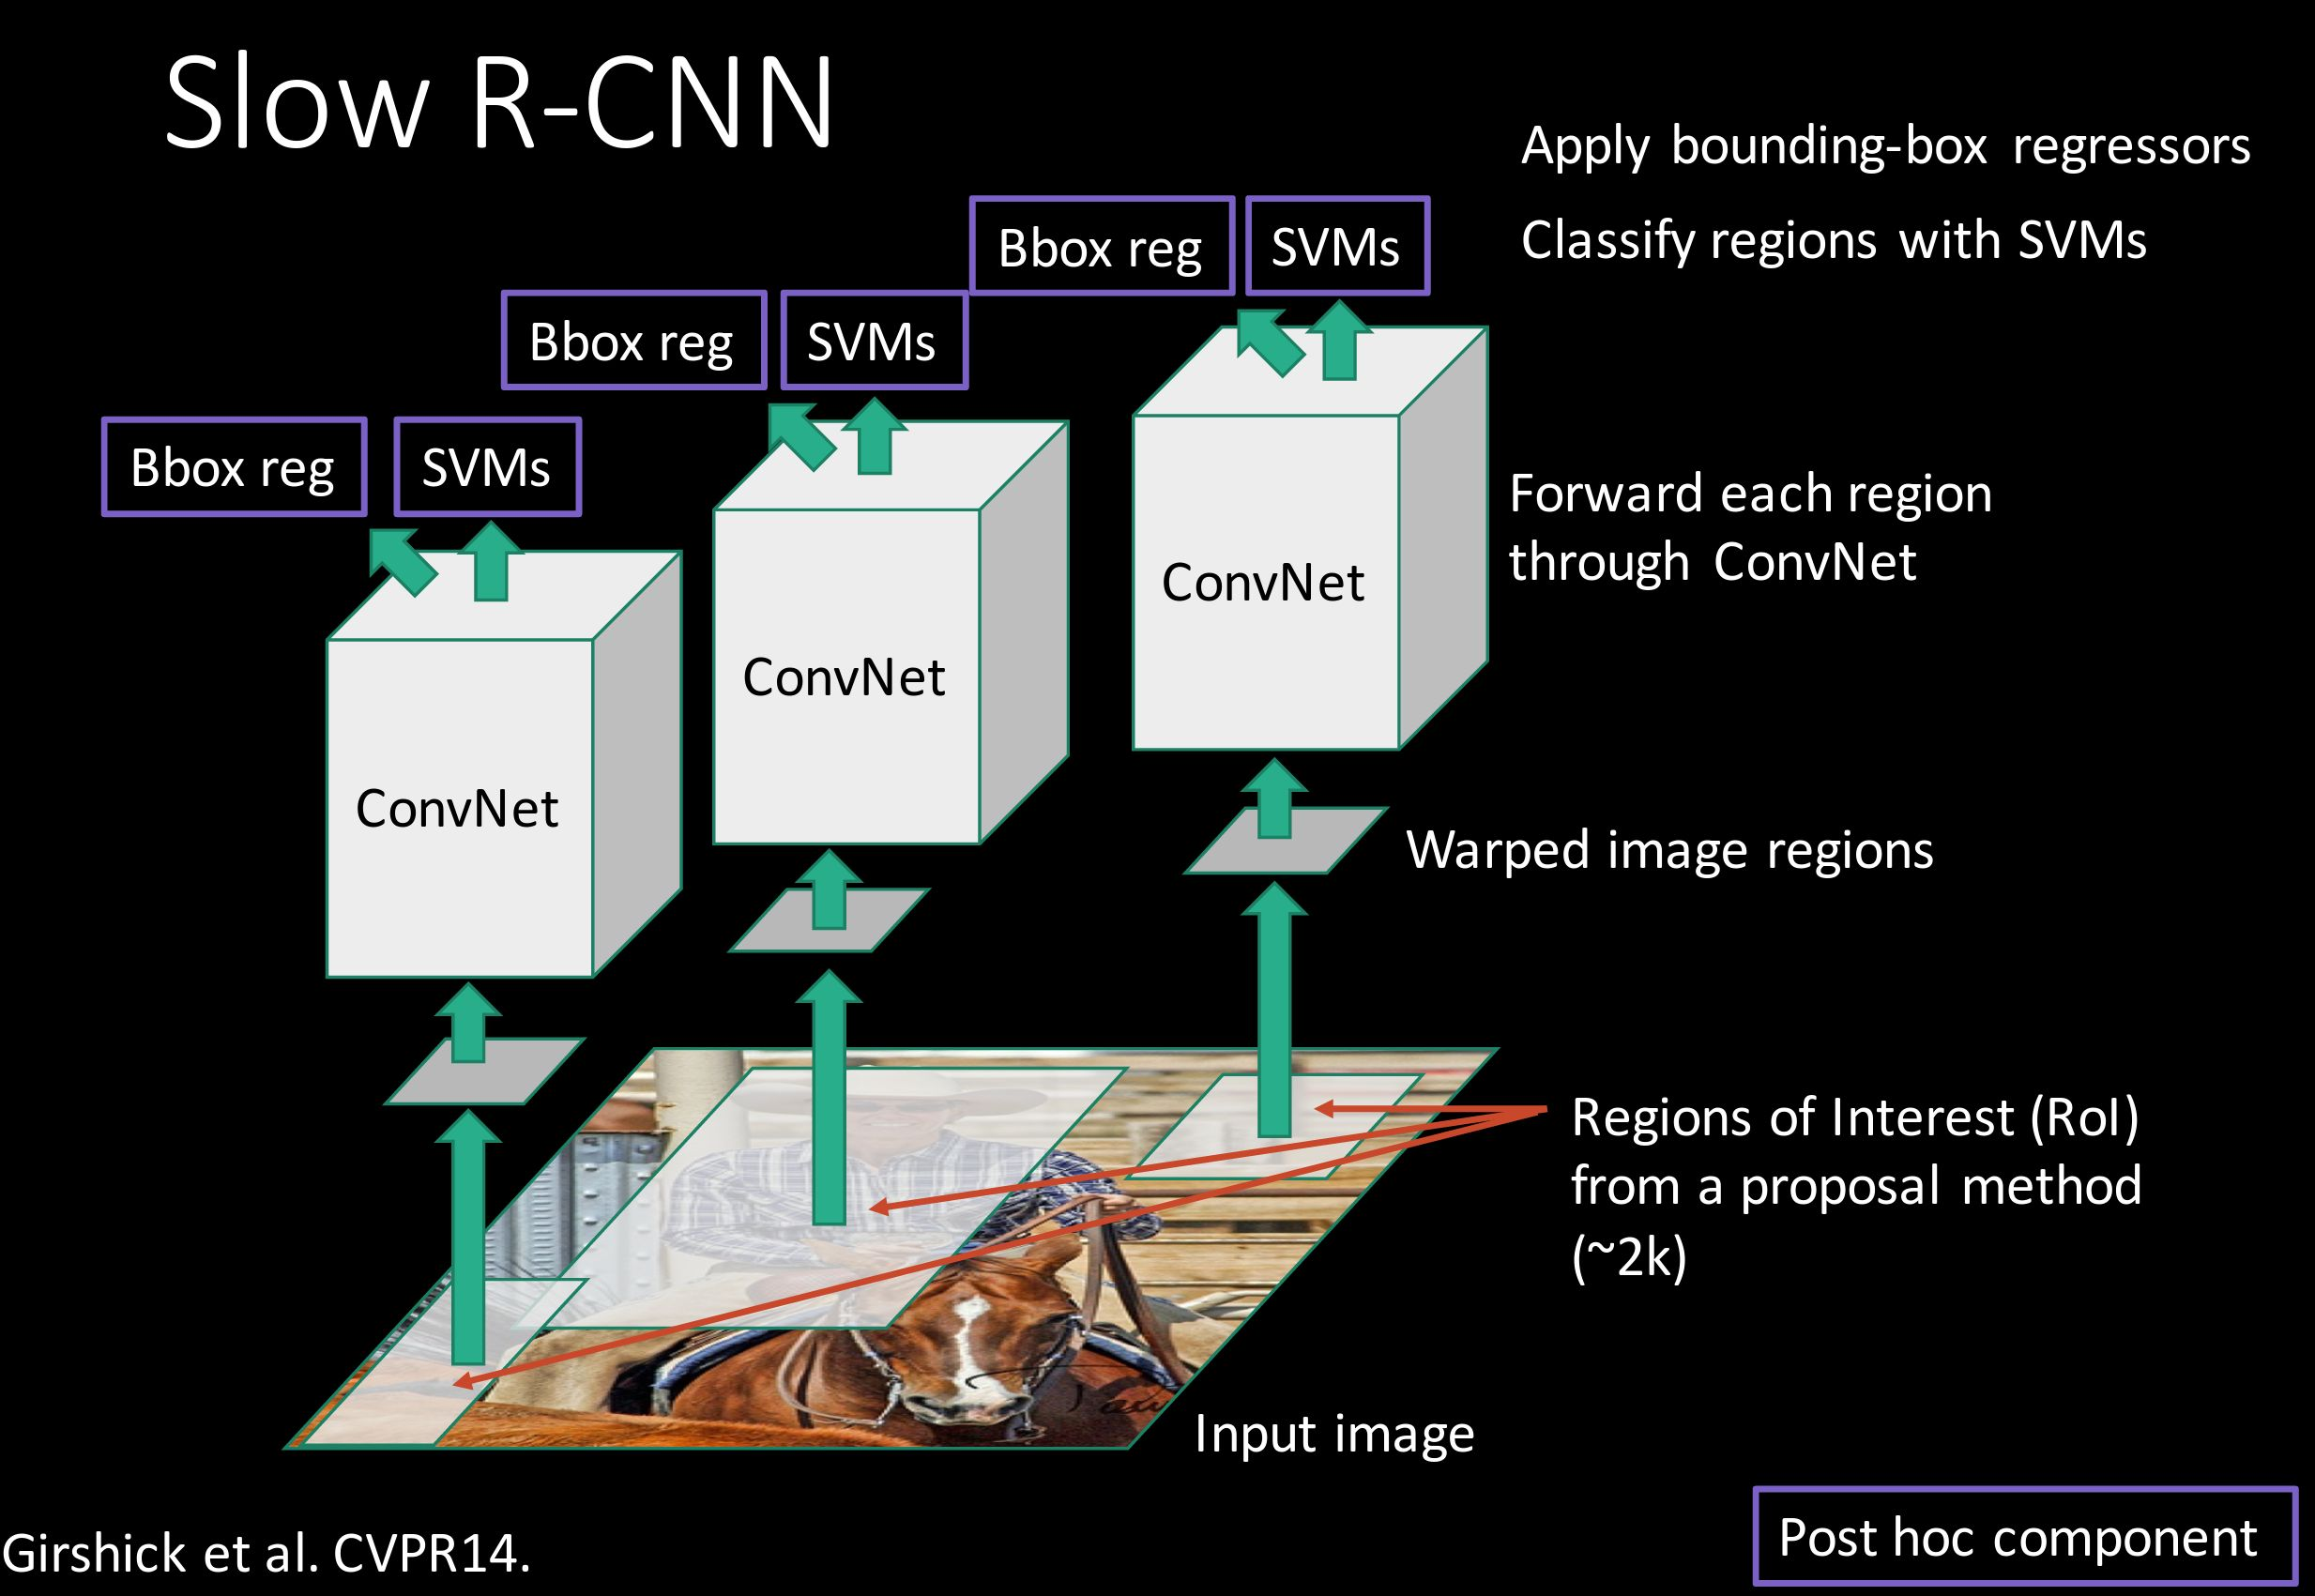
\includegraphics[height=.8\textheight]{rcnn}
\end{frame}

\begin{frame}
  \frametitle{R-CNN: results}
  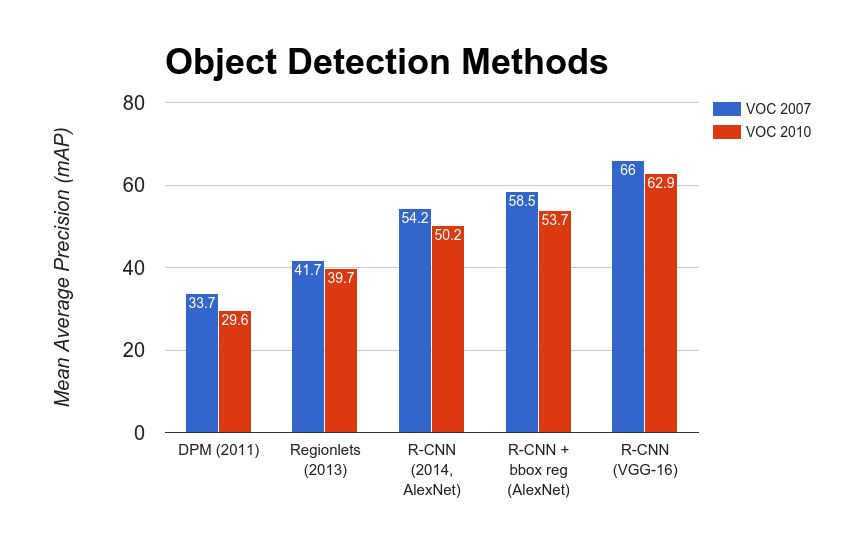
\includegraphics[width=.8\textwidth]{rcnn-results}
\end{frame}

\begin{frame}
  \frametitle{Fast RCNN}
  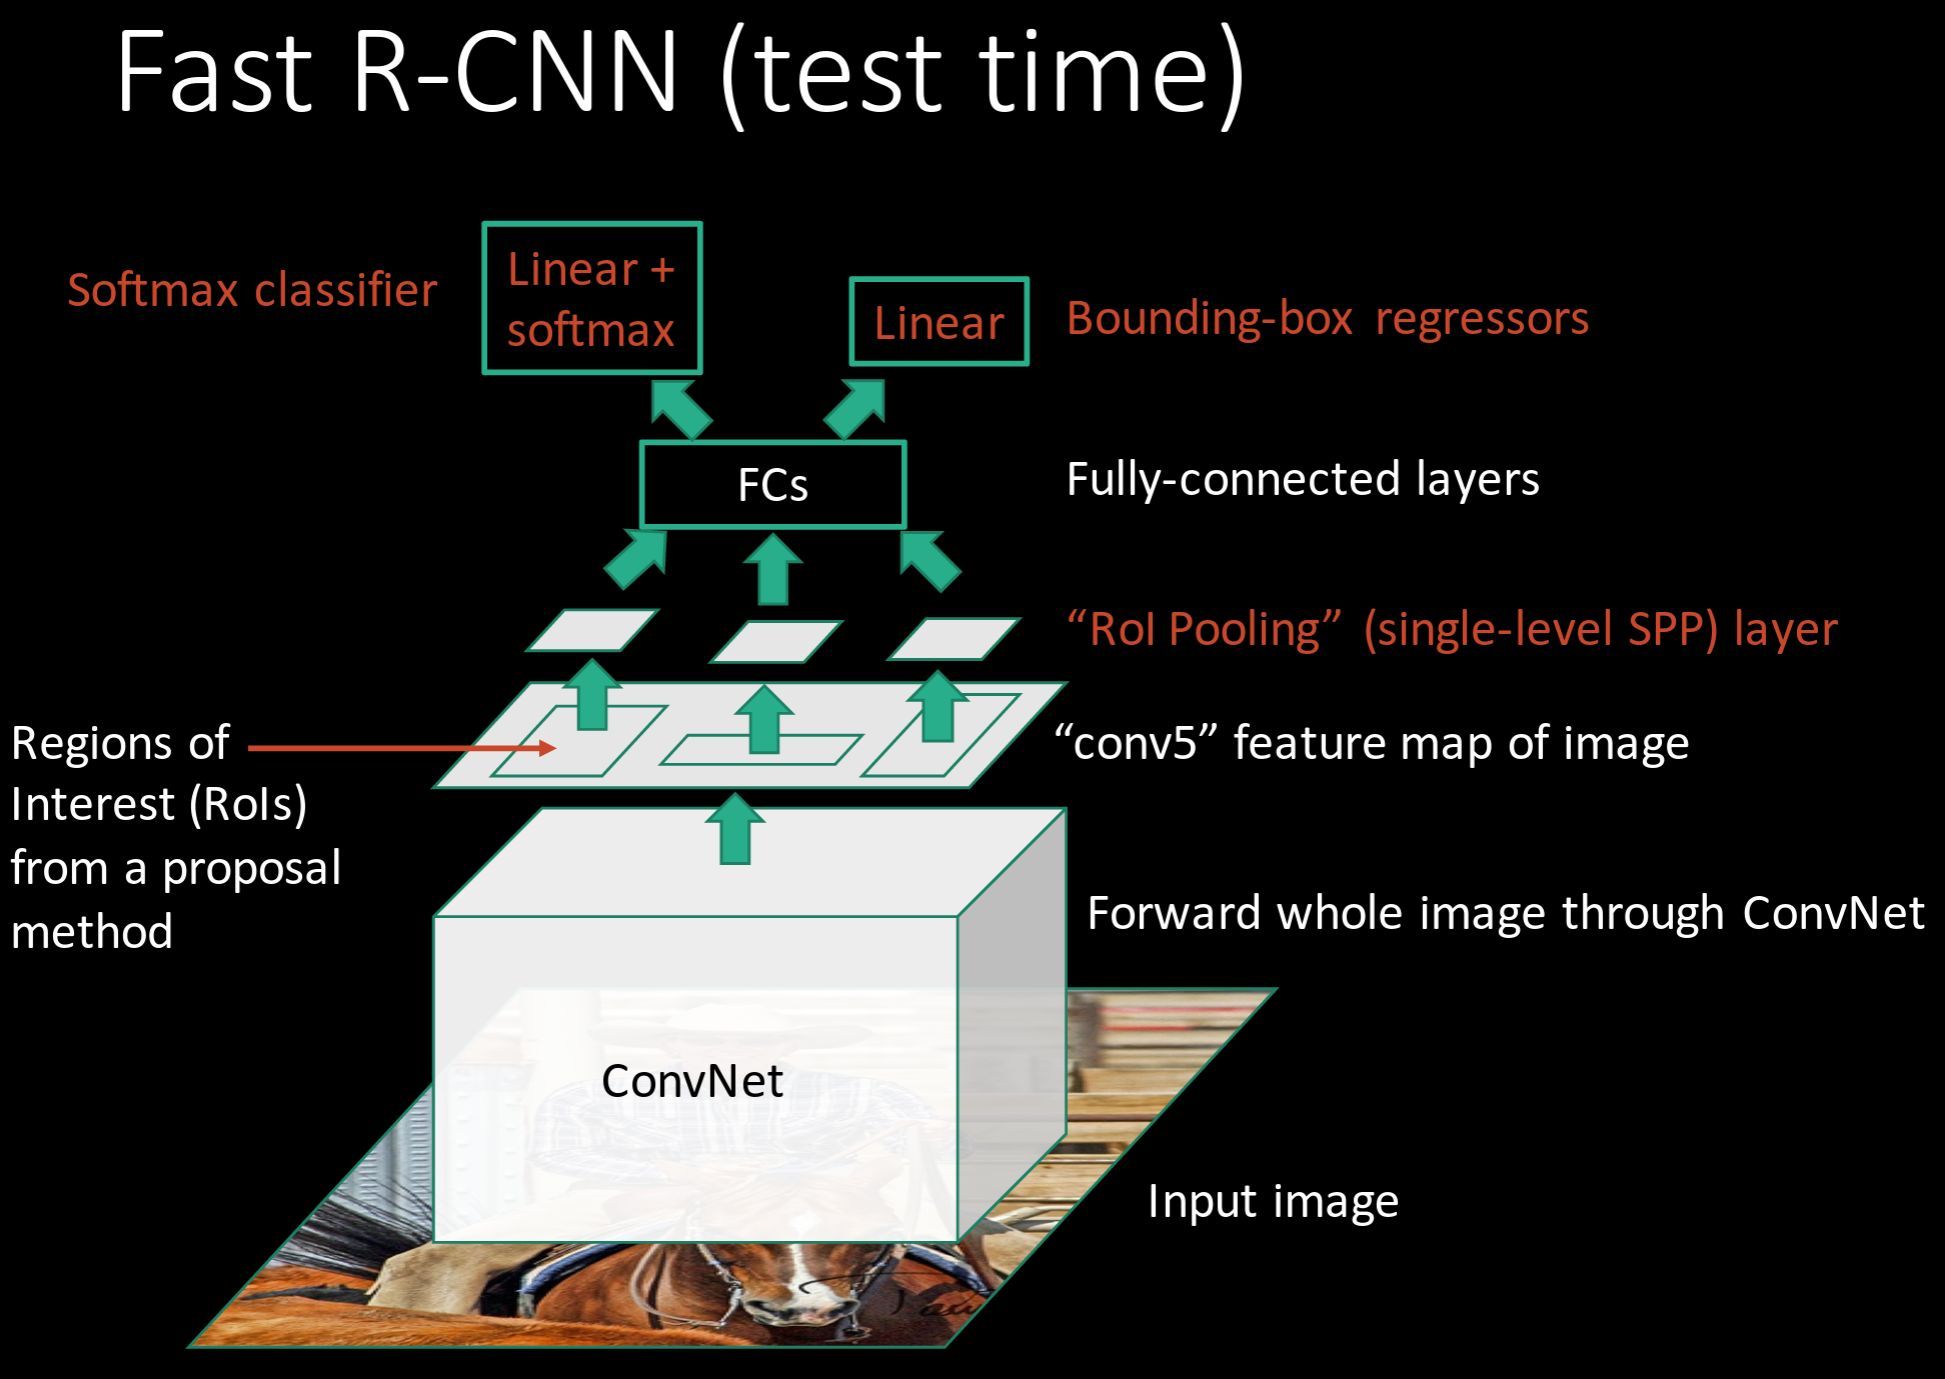
\includegraphics[height=.8\textheight]{fast-rcnn-test}
\end{frame}


\begin{frame}
  \frametitle{Fast RCNN}
  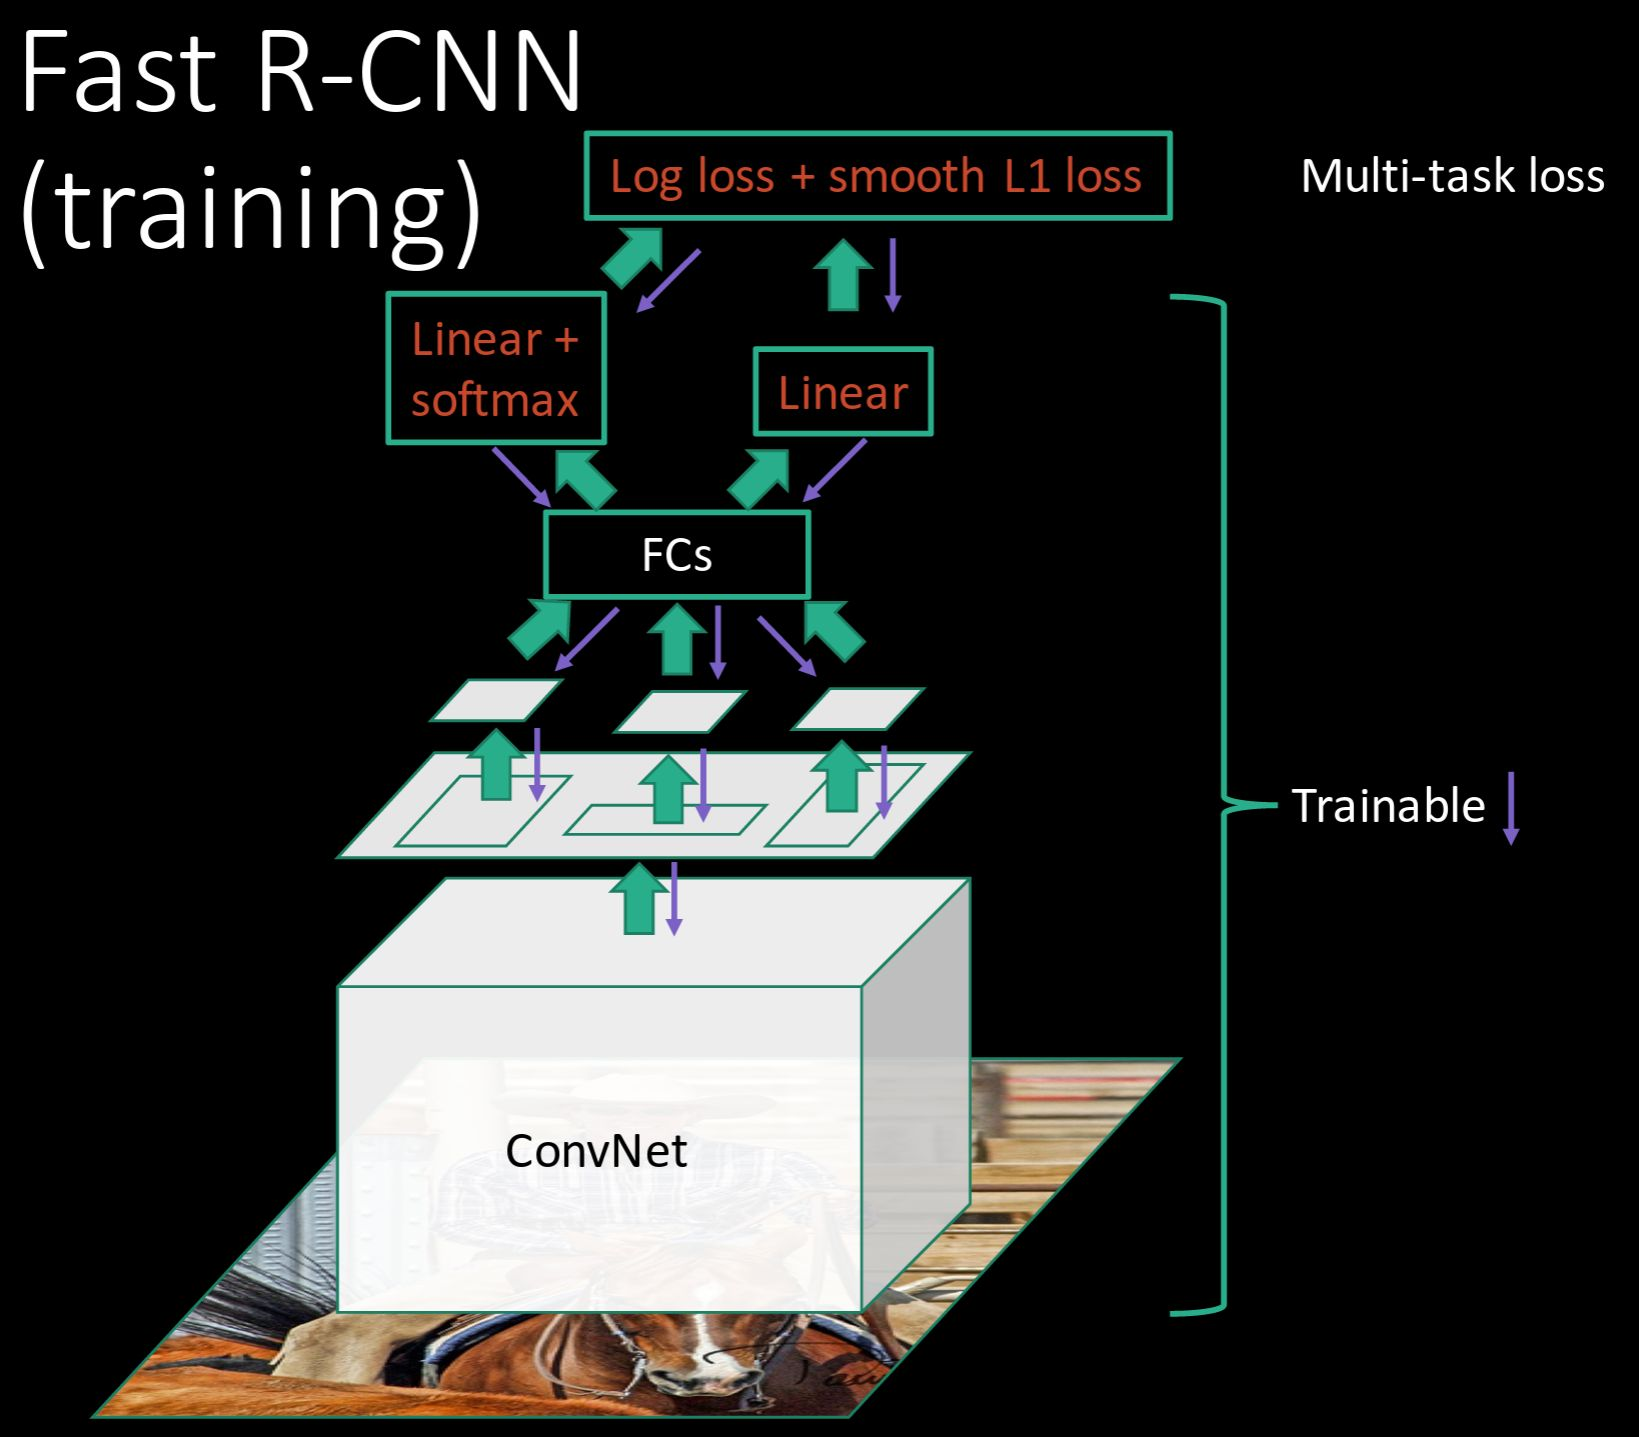
\includegraphics[height=.8\textheight]{fast-rcnn-train}
\end{frame}


\begin{frame}
  \frametitle{Fast RCNN: ROI pooling}
\bi
\item Project region proposal to feature map
\item Pool within each grid cell
\ei
  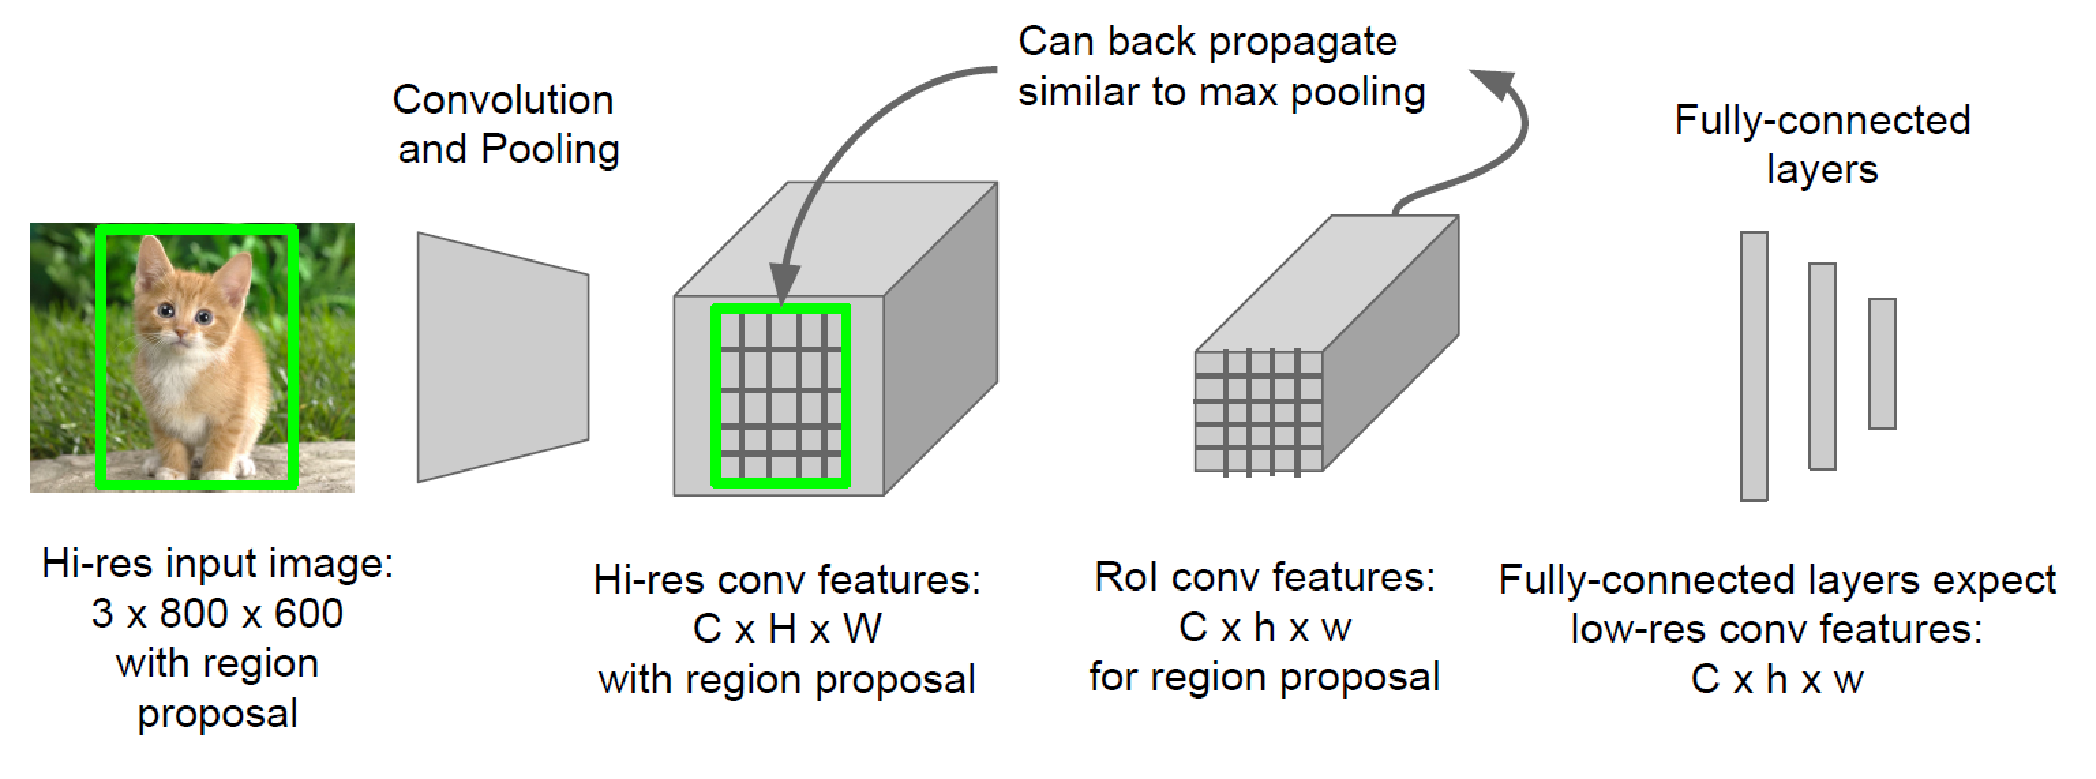
\includegraphics[width=.9\textwidth]{fast-rcnn-roi-pooling}
\end{frame}

\begin{frame}
  \frametitle{Fast RCNN results}
  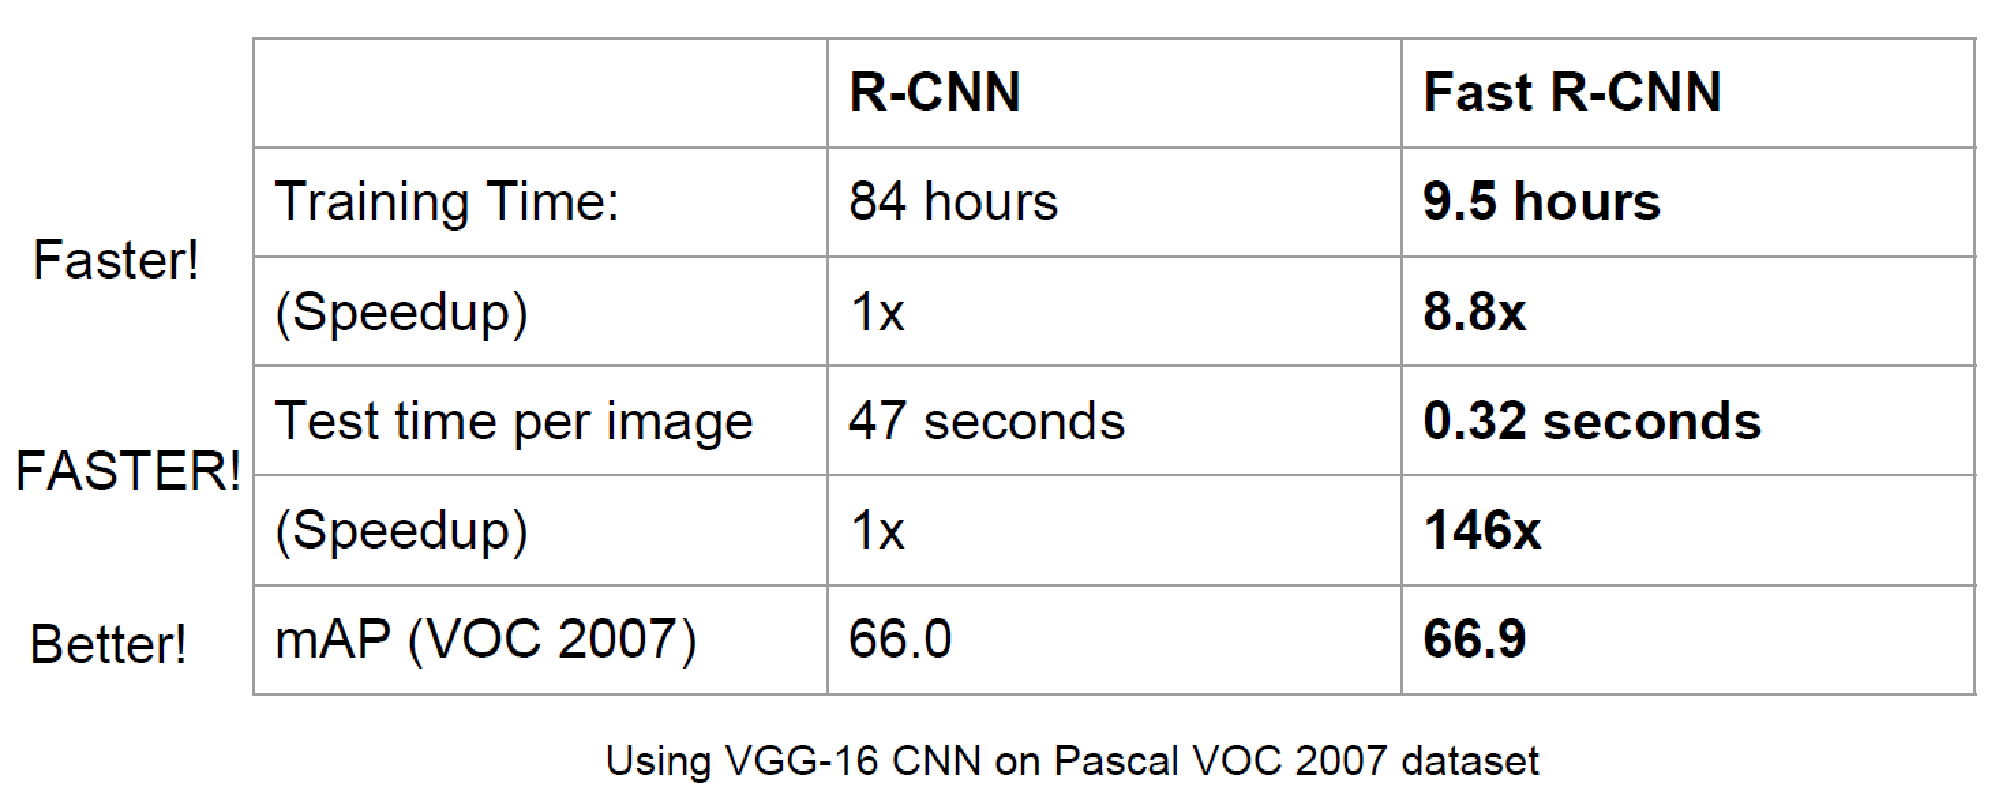
\includegraphics[width=.8\textwidth]{fast-rcnn-results}
\end{frame}

\begin{frame}
  \frametitle{Faster RCNN}
  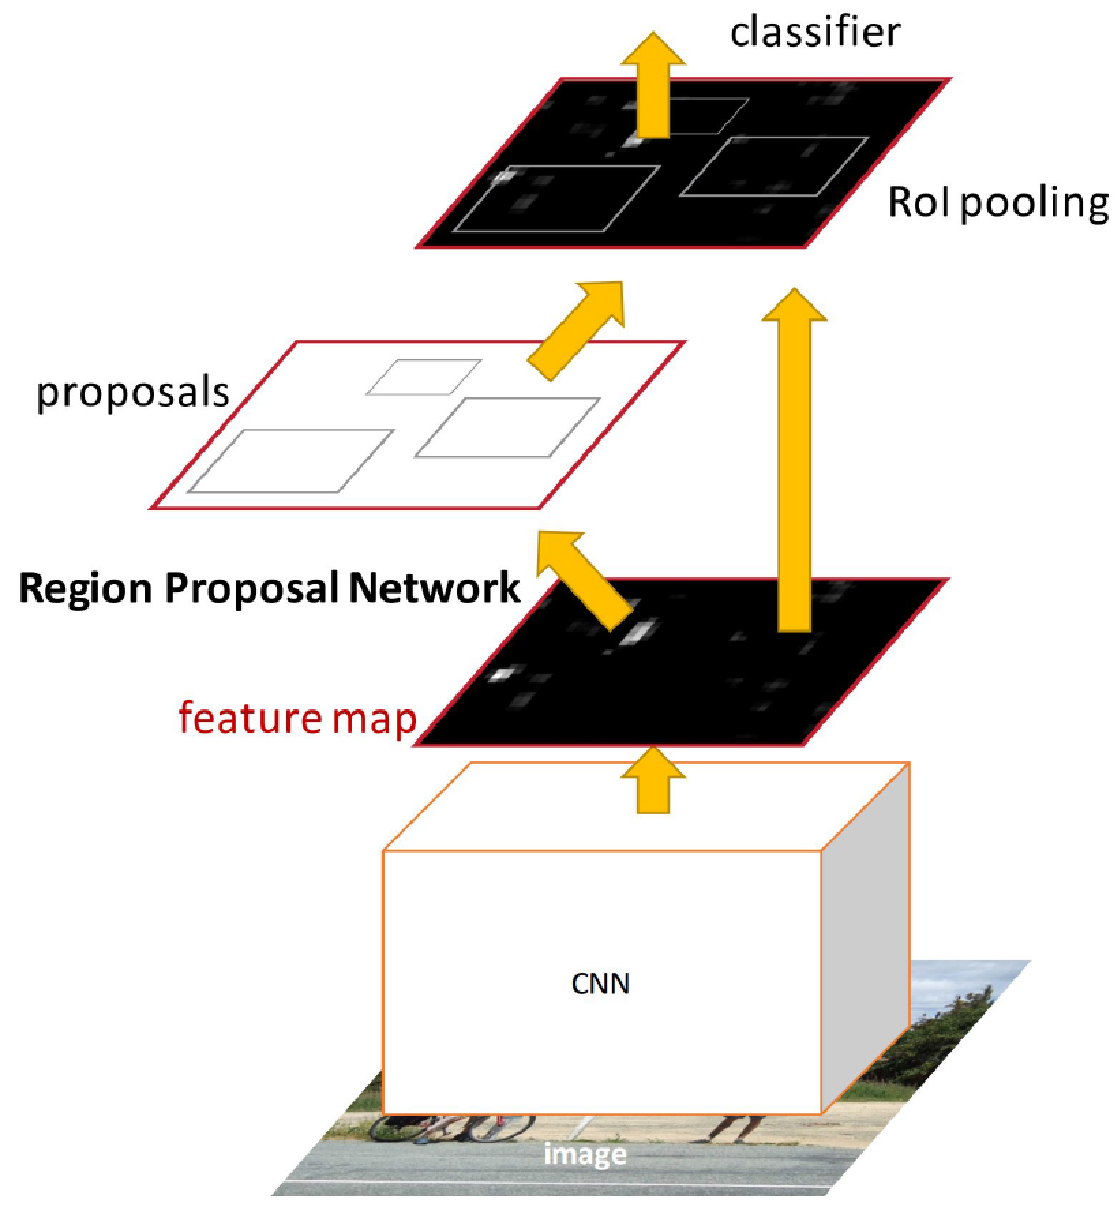
\includegraphics[width=.5\textwidth]{faster-rcnn-test}
  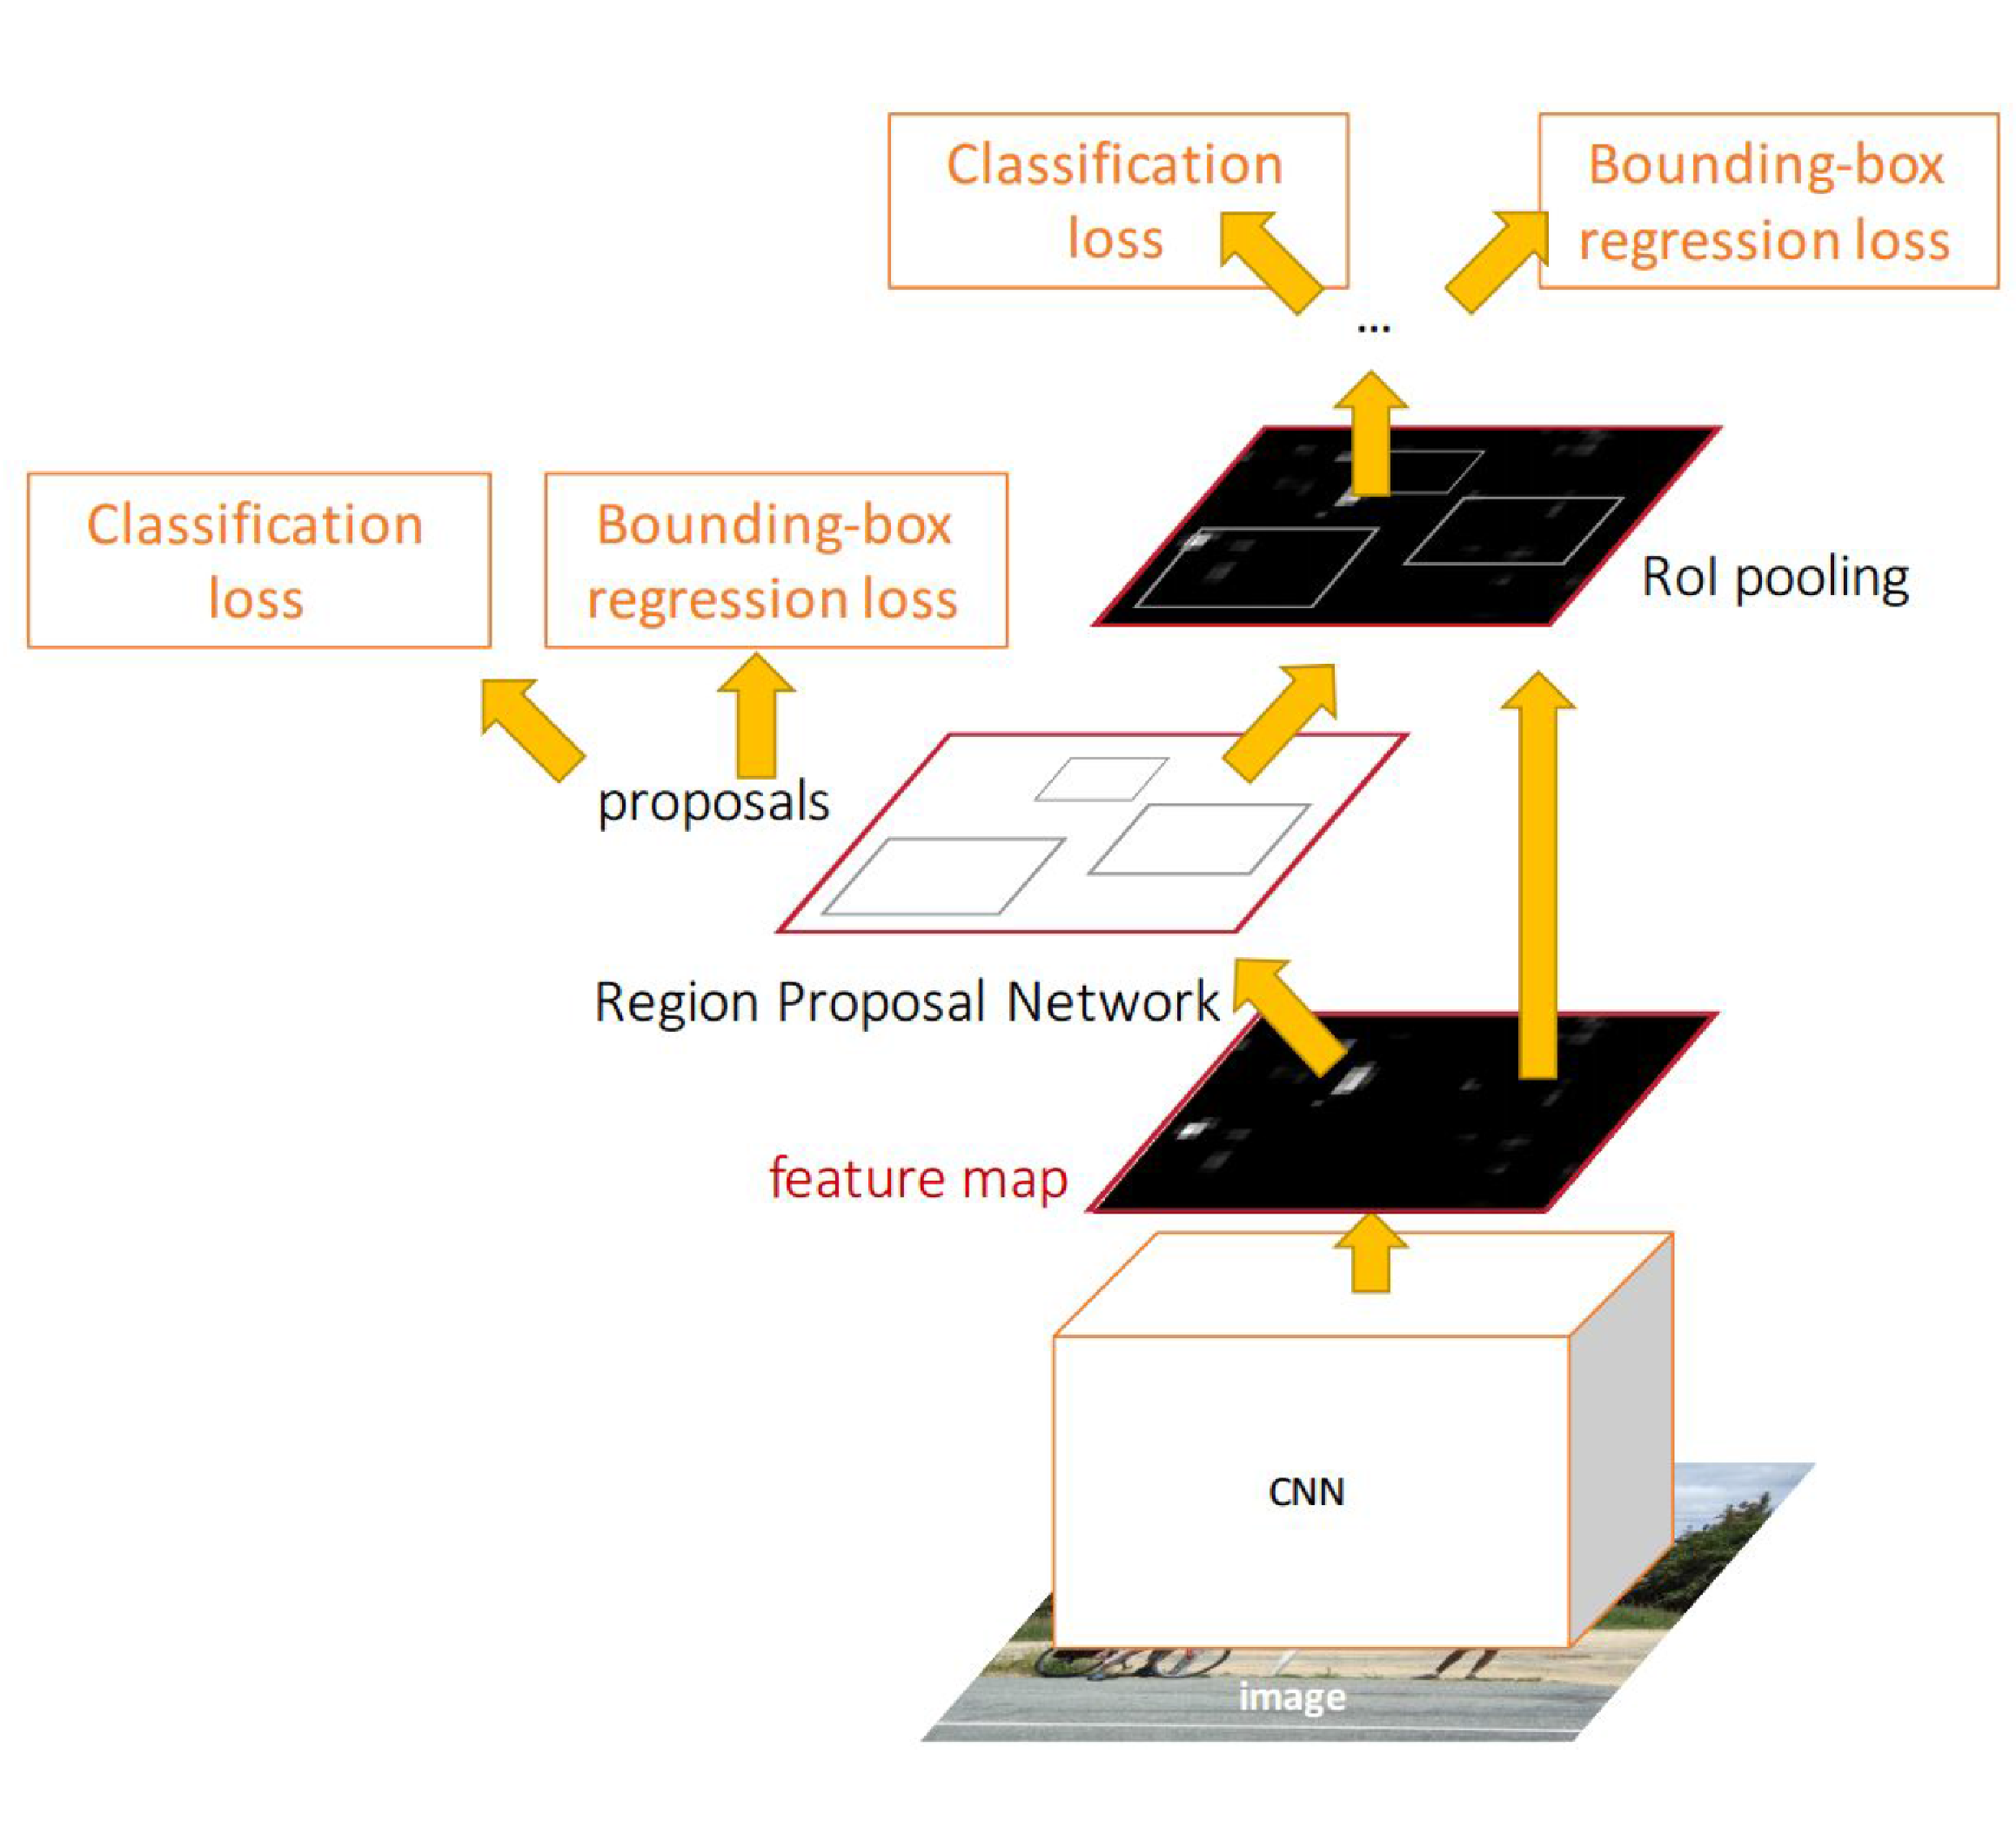
\includegraphics[width=.5\textwidth]{faster-rcnn-train}
\end{frame}

\begin{frame}
  \frametitle{Region proposal network}
  \bi
\item Learn to choose and refine coarse proposals
\item Use a few ``anchors'' with diff. aspect ratios
\ei
  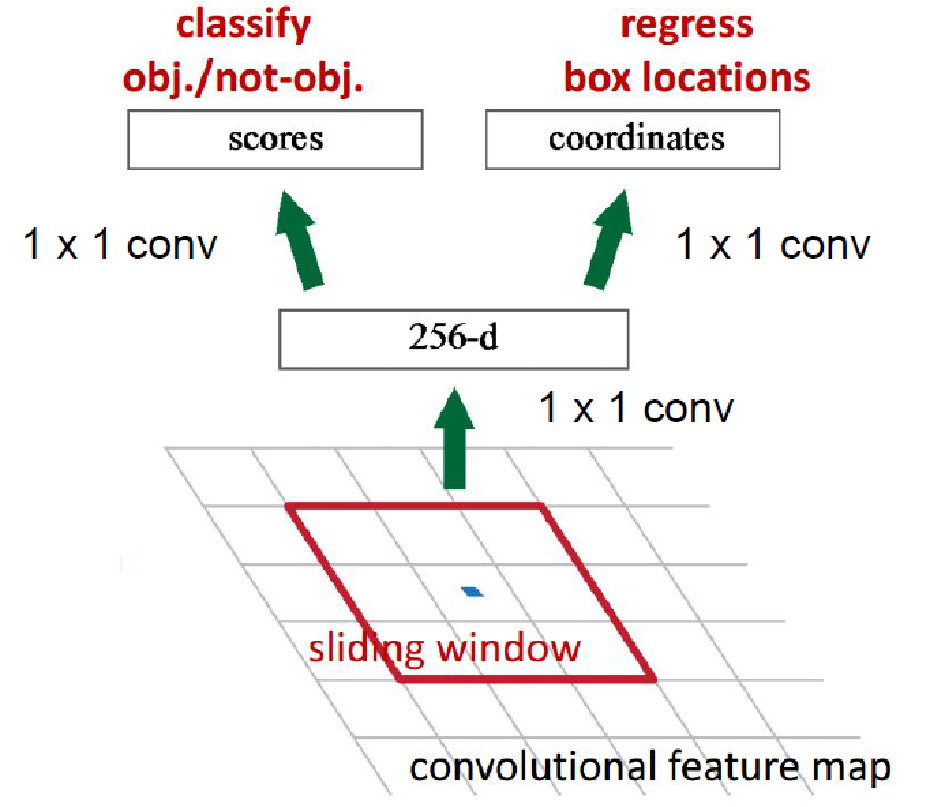
\includegraphics[width=.45\textwidth]{rpn-1}
  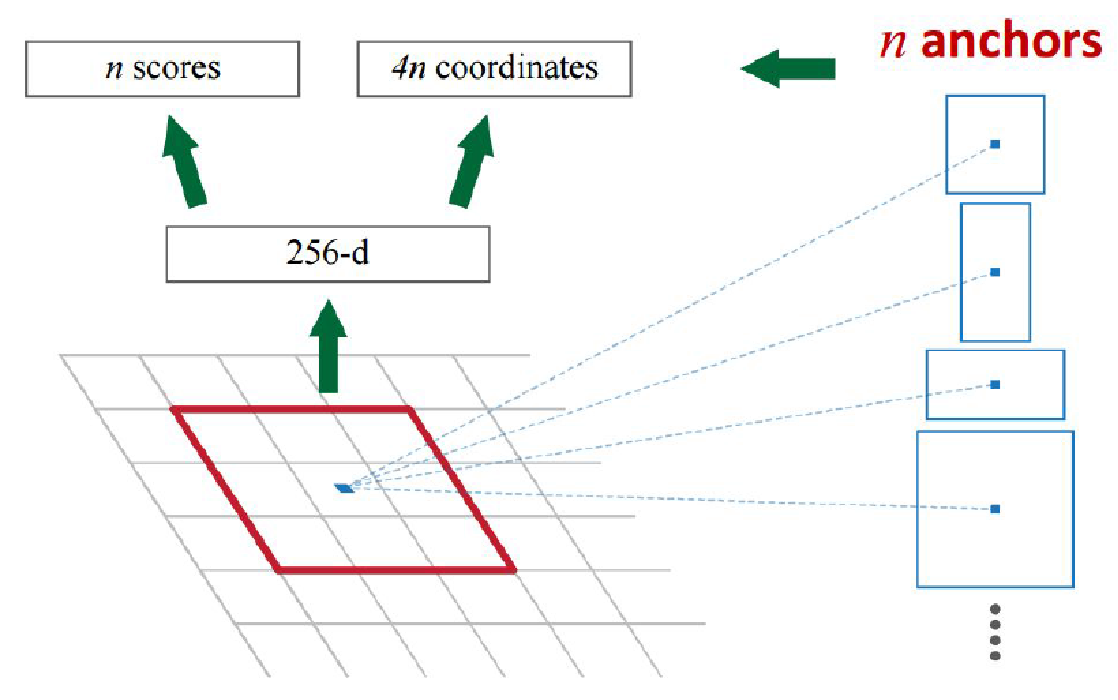
\includegraphics[width=.53\textwidth]{rpn-2}
\end{frame}


\begin{frame}
  \frametitle{Hypercolumns for image labeling}
  \begin{tikzpicture}
\def\winput{3.0}
\def\hinput{2.4}
\def\winputlow{1.5}
\def\hinputlow{1.2}
\action<1->{
  
  \node[inner sep=0pt,transform shape] (input) at (0,0)
  {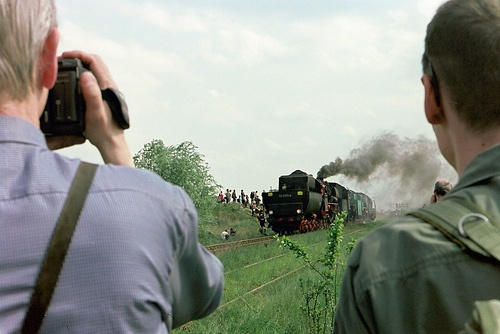
\includegraphics[width=\winput cm,height=\hinput cm]{figs/2007_002728.jpg}};
  
  \def\xoffset{-0.5}
  \def\yoffset{-0.6}
  \def\xshift{0.15}
  \def\yshift{0.20}
  \def\toptext{3.0}
  
  \node[circle,inner sep=.04cm,fill=red] (input-pixel) at (\xoffset*\winput/2, \yoffset*\hinput/2) {};
  % \node[white,anchor=east] at (input-pixel) {$p$};
  
  \node[black,anchor=north] at (0,-\hinput/2-0.05)
  {\scriptsize{\textbf{\textsf{Input image}}}};
}


%\filldraw[yellow!50, draw=black, opacity=0.75] (0.7,1.8) rectangle (1.9,3.1);
%\filldraw[yellow!50, draw=black, opacity=0.75] (1.0,2.3) rectangle (2.0,3.3);
%\filldraw[yellow!50, draw=black, opacity=0.75] (1.2,2.6) rectangle (2.2,3.6);

\def\scale{0.00029}
\def\hfoot{-0.6}
\def\hcenter{\hfoot+6028*\scale + 0.25}
\def\bsize{1.3}
\def\bapart{2.0}

\action<2-> {
  \foreach \s/\c in {1/0, 64/1, 64/65, 128/129, 128/257, 256/385, 256/641, 256/897, 512/1153, 512/1665, 512/2177, 512/2689, 512/3201, 512/3713, 4096/4225, 4096/8321} {
    \filldraw[purple!50, draw=black!50!purple, opacity=0.95,thin] (3,\hfoot + \c*\scale) rectangle (3.3,\hfoot + \c*\scale+\s*\scale);
    
  }
  \node[black,anchor=south] at (0,\toptext) {\scriptsize{\textbf{\textsf{VGG-16}}}};  

}

\foreach \id/\s/\hw/\name/\y/\bend/\ba in {
  a/3/1.2/{\scriptsize{\textsf{conv1\_1}}}/{\hfoot+\scale*33}/-20,
  b/8.2/0.55/{\scriptsize{\textsf{conv5\_3}}}/{\hfoot+\scale*3969}/-40,
  c/10.3/0.5/{\scriptsize{\textsf{(fc6) conv6}}}/{\hfoot+\scale*6273}/-30,
  d/12/0.5/{\scriptsize{\textsf{(fc7) conv7}}}/{\hfoot+\scale*10369}/20} {
  \action<2-> {
    \filldraw[yellow!20,draw=black,opacity=0.8,thin] (\s*\xshift-\hw,\s*\yshift-\hw) rectangle (\s*\xshift+\hw,\s*\yshift+\hw);
    \node[anchor=north east] at (\s*\xshift-\hw, \s*\yshift+\hw+0.1) {\tiny{\name}};
  }
  \action<4-> {
    \node[circle,inner sep=.04cm,fill=red] (node\id) at (\s*\xshift + \xoffset*\hw, \s*\yshift + \yoffset*\hw) {};
    \draw[black,-latex,thick,out=\ba,in=180] (node\id) to (3,\y);
  }
}

\action<2-> {
  \foreach \s in {2.5, 3, 3.5} {
    \node[circle,inner sep=.02cm,fill=black] at (\s*\xshift, \s*\yshift) {};
  }
}

\action<3-> {
  \node[anchor=south] at (3.15, \toptext) {\scriptsize{\textbf{\textsf{Hypercolumn}}}};
}
%\node[anchor=north] at (3.15, \hfoot) {\scriptsize{12,417}};

\action<4-> {
\filldraw[purple!50, draw=black!50!purple, thin, opacity=0.95]
(3.8,\hcenter - 512*\scale) rectangle (4.1,\hcenter + 512*\scale);

\filldraw[purple!50, draw=black!50!purple, thin, opacity=0.95]
(4.6,\hcenter - 512*\scale) rectangle (4.9,\hcenter + 512*\scale);

\filldraw[purple!50, draw=black!50!purple, thin, opacity=0.95]
(5.4,\hcenter - 21*\scale) rectangle (5.7,\hcenter + 21*\scale);

\draw[black,thick,-latex](3.3, \hcenter) to (3.8,\hcenter);
\draw[black,thick,-latex](4.1, \hcenter) to (4.6,\hcenter);
\draw[black,thick,-latex](4.9, \hcenter) to (5.4,\hcenter);

\node[anchor=south] at (3.95, \hcenter + 512*\scale) {\scriptsize{\textsf{h\_fc1}}};
\node[anchor=south] at (4.75, \hcenter + 512*\scale)
{\scriptsize{\textsf{h\_fc2}}};
\node[anchor=south] at (5.55, \hcenter + 21*\scale) {\scriptsize{\textsf{cls}}};
%\node[anchor=north] at (4.15, \hfoot + 6208*\scale - 512*\scale) {\scriptsize{1024}};
}

\action<5,7>{

  \node[black,anchor=north] at (8,-\hinput/2-0.05)
  {\scriptsize{\textbf{\textsf{Output map}}}};
  
  \node[inner sep=0pt,transform shape] (output) at (8,0)
  {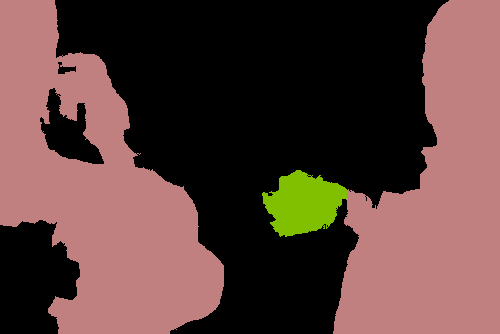
\includegraphics[width=\winput cm,height=\hinput cm]{figs/2007_002728.png}};
  
  % point in output map
  \node[circle,inner sep=.04cm,fill=red] (output-pixel) at (8+\xoffset*\winput/2, \yoffset*\hinput/2) {};
}
\action<5>{
  \draw[gray,thick,-latex,out=0,in=135](5.7, \hcenter) to (output-pixel);
}


\action<6->{
  \node[black,anchor=north] at (8,5.5-\hinput/2-0.05)
  {\scriptsize{\textbf{\textsf{Output map (low res)}}}};
  
  \node[inner sep=0pt,transform shape] (output-lowres) at (8,3)
  {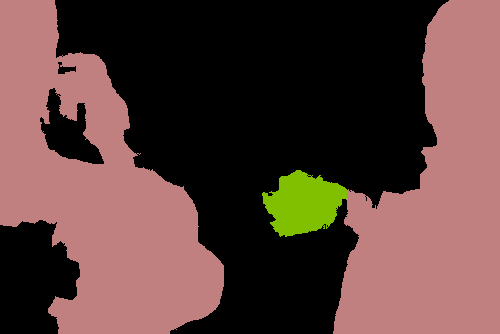
\includegraphics[width=\winputlow cm,height=\hinputlow cm]{figs/2007_002728.png}};

  \node[circle,inner sep=.04cm,fill=red] (output-pixel-low) at
  (8+\xoffset*\winputlow/2, 3+\yoffset*\hinputlow/2) {};
  
  \draw[black,thick,-latex,out=0,in=-135](5.7, \hcenter) to (output-pixel-low);

  \draw[black,thick,-latex] (output-lowres) -- (output) node[midway,left] {\textbf{\textsf{$\uparrow\,2$}}};
}


\end{tikzpicture}
\bi\item Hypercolumns: skip-layer connections from lower layers
directly to classification network\\
{[Mostajabi et al., 2015]}
\ei

\end{frame}


\begin{frame}
  \frametitle{Dilated convolution}
  \bi
\item Problem with fully-convolutional nets: large stride
\item One solution: \emph{a-trous} (hole) convolution

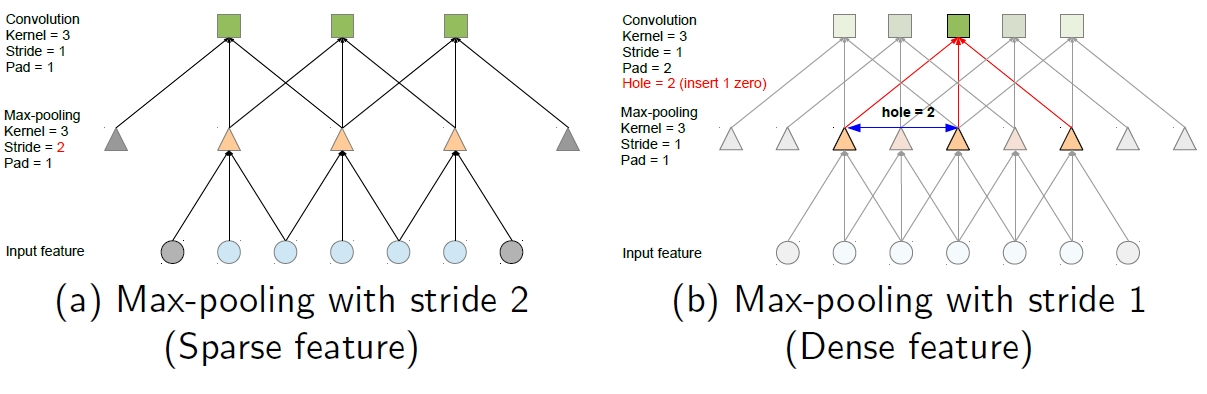
\includegraphics[width=.8\textwidth]{atrous_example2}
\\{[Chen et al.]}
\ei
\end{frame}

\section{Recurrent networks}


\begin{frame}
  \frametitle{Recurrent networks}  
  \bi
\item Ostensibly, RNNs depart from the DAG assumption:
\begin{align*}
\mathbf{h}^{(0)}&=F_0(\vx;\Theta_0)\\
\mathbf{h}^{(t)}&=F(\vx,\mathbf{h}^{(t-1)};\Theta)
\end{align*}

\item This is a dynamical system governed (after initialization) by
  $F$
\item However, in terms of neural network this simply means that the
  parameters are shared between time frames.
\item Vanilla RNN (with single input):
  \begin{align*}
    \mathbf{h}^{(0)}\,&=\,g(\mathbf{W}_{xh}\vx+\mathbf{b}_0)\\
    \mathbf{h}^{(t)}\,&=\,g\left(\mathbf{W}_{xh}\vx+\textcolor{red}{\mathbf{W}_{hh}}\mathbf{h}^{(t-1)}+\mathbf{b}_h\right)
  \end{align*}
\ei
\end{frame}


\begin{frame}
  \frametitle{Unrolling RNNs}
\begin{align*}
    \mathbf{h}_t\,&=\,g(\mathbf{W}_{xh}\vx+\mathbf{b}_0)\\
    \mathbf{h}_t\,&=\,g\left(\mathbf{W}_{xh}\vx+\textcolor{red}{\mathbf{W}_{hh}}\mathbf{h}_{t-1}+\mathbf{b}_h\right)
  \end{align*}
  \bi
\item For a given number of time frames (steps), we can \emph{unroll}
  this to a ``normal'' deep neural network

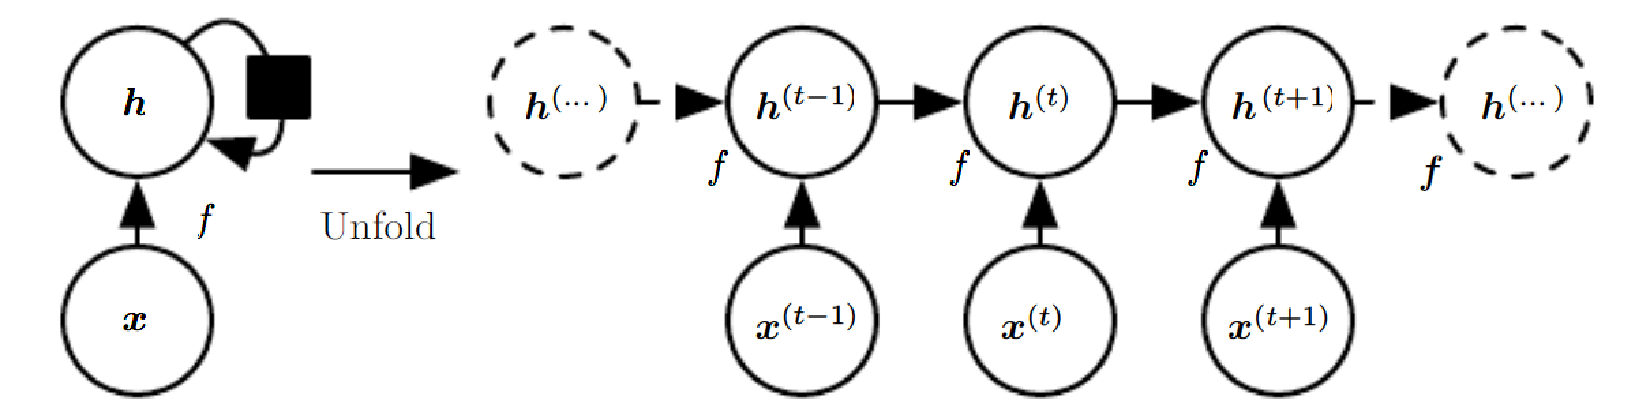
\includegraphics[width=.8\textwidth]{gcb-rnn-unfold}
\raisebox{1em}{\hspace{-4em}[Goodfellow et al.]}

with the constraing that $\mathbf{W}_{hh}$ are tied across layers.
\ei
\end{frame}

\begin{frame}
  \frametitle{Many forms of RNNs}

  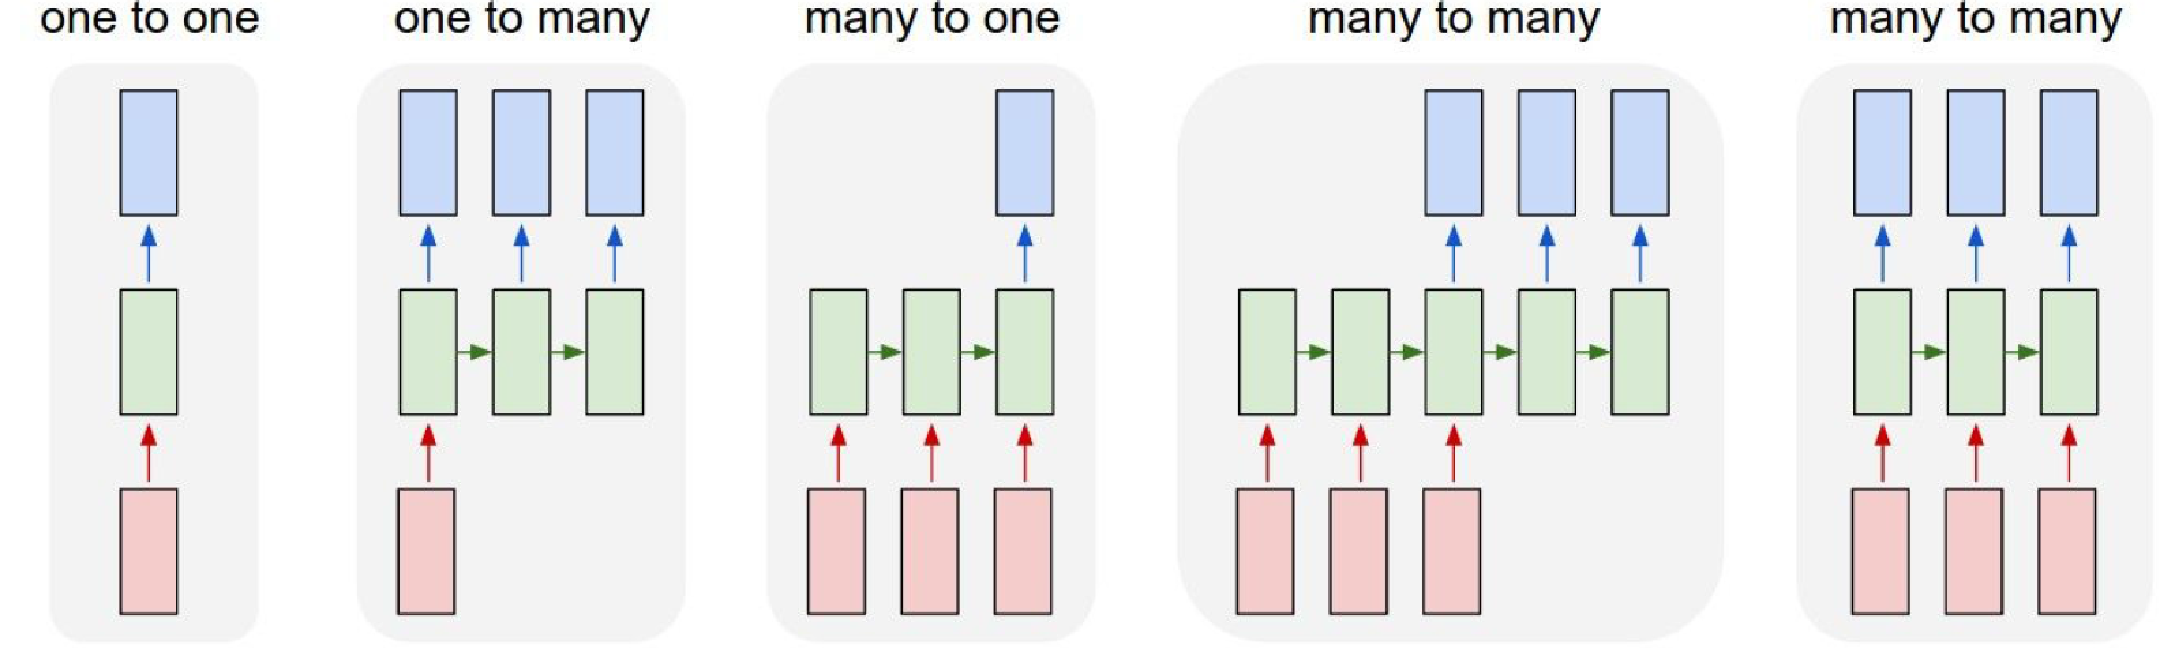
\includegraphics[width=.95\textwidth]{ak-rnn-forms}\\

[A. Karpathy]
\bi
\item One-to-one: ``normal'' neural net
\item One-to-many: image captioning (one image to sequence of words)
\item Many-to-one: sequence classification (e.g., sentiment analysis)
\item Many-to-many: machine translation (sequence to another
  sequence), or frame classification (e.g., video), frame per frame
\ei
\end{frame}


\begin{frame}
  \frametitle{Training sequence labeler}
  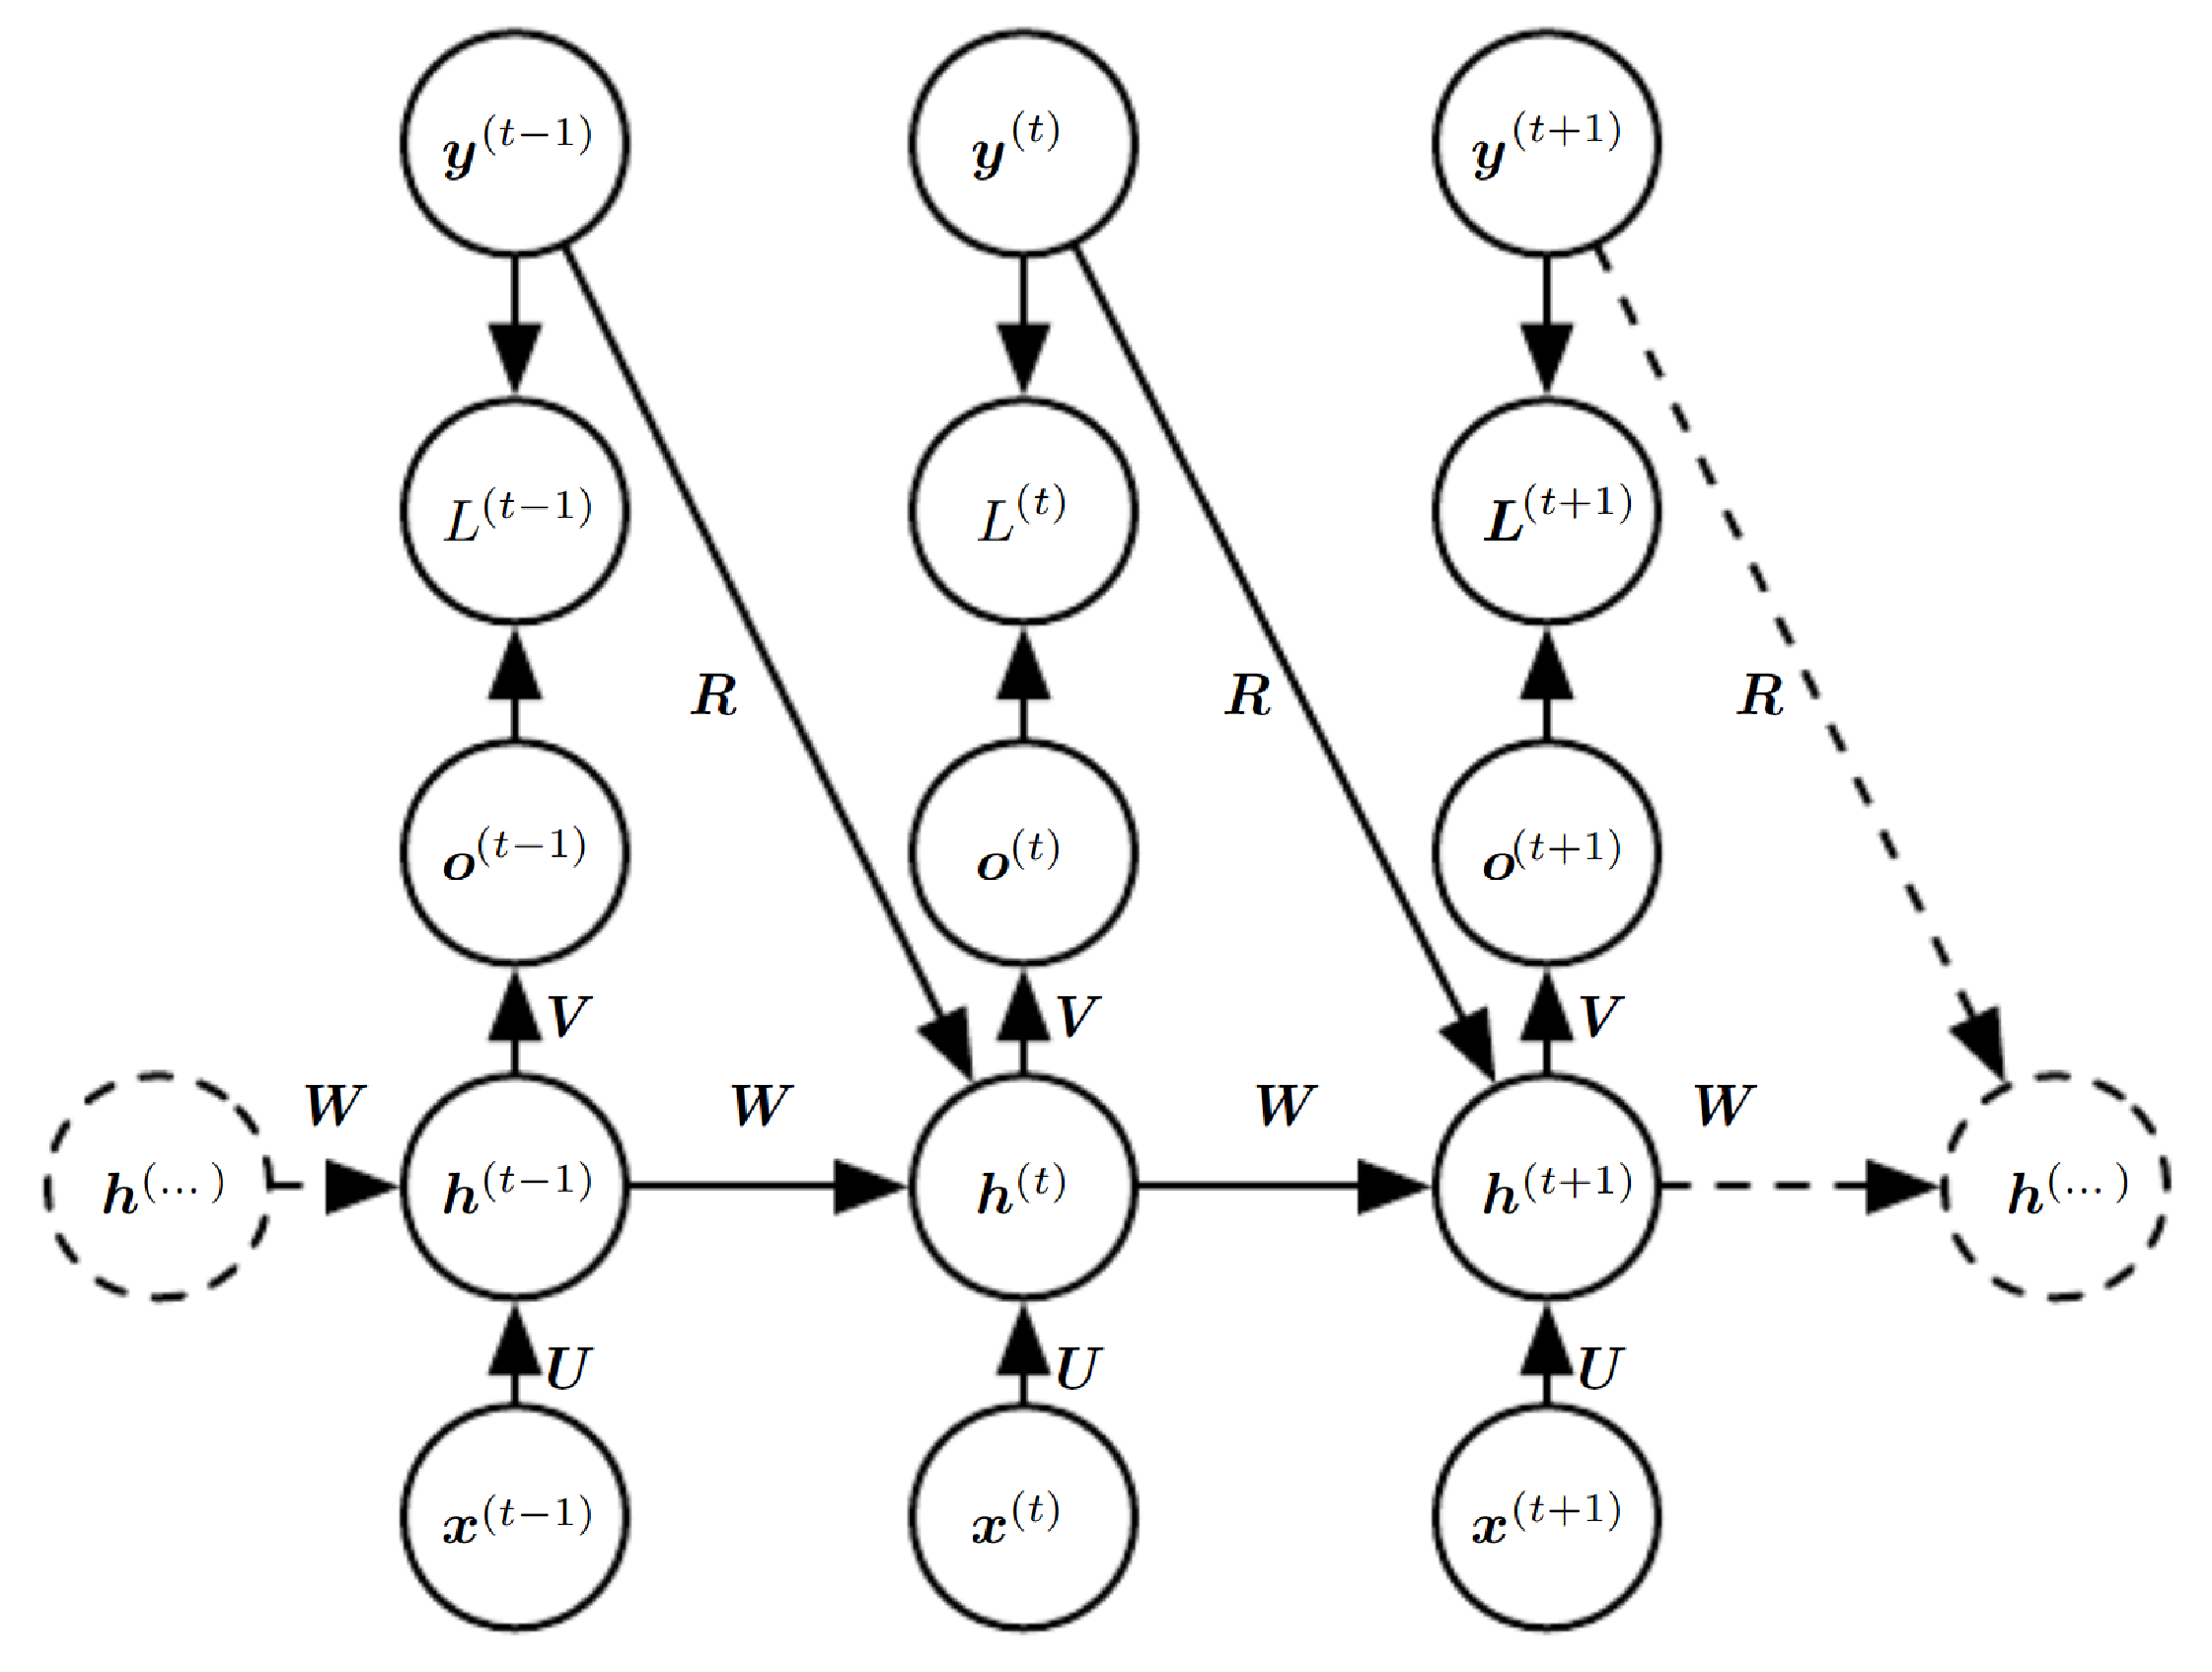
\includegraphics[width=.6\textwidth]{gcb-rnn-seq2seq-fixedlen}\raisebox{1em}{[Goodfellow
  et al.]}
\bi
\item Loss is computer per frame (typically cross-entropy)
\item $\mathbf{R}$ allows for modeling structure (conditional
  dependencies between $y$s given $\vx$)
\ei
\end{frame}

\begin{frame}
  \frametitle{Example: character-level language model}
  \bi
\item Input: previous character, output: next character
\item Input characters $\vx_t$: one-hot encoding
\ei
\begin{minipage}[c]{.5\linewidth}
  \bi
\item Hidden layer:
\[\mathbf{h}_t=\tanh\left(\mathbf{W}_{hh}\mathbf{h}_{t-1}+\mathbf{W}_{xh}\vx_t\right)
\]
\item Output
\[\mathbf{o}_t=\mathbf{W}_{hy}\mathbf{h}_t
\]
\item Word $y_t$ drawn from softmax($\mathbf{o}_t$)
\ei
\end{minipage}%
\begin{minipage}[c]{.5\linewidth}
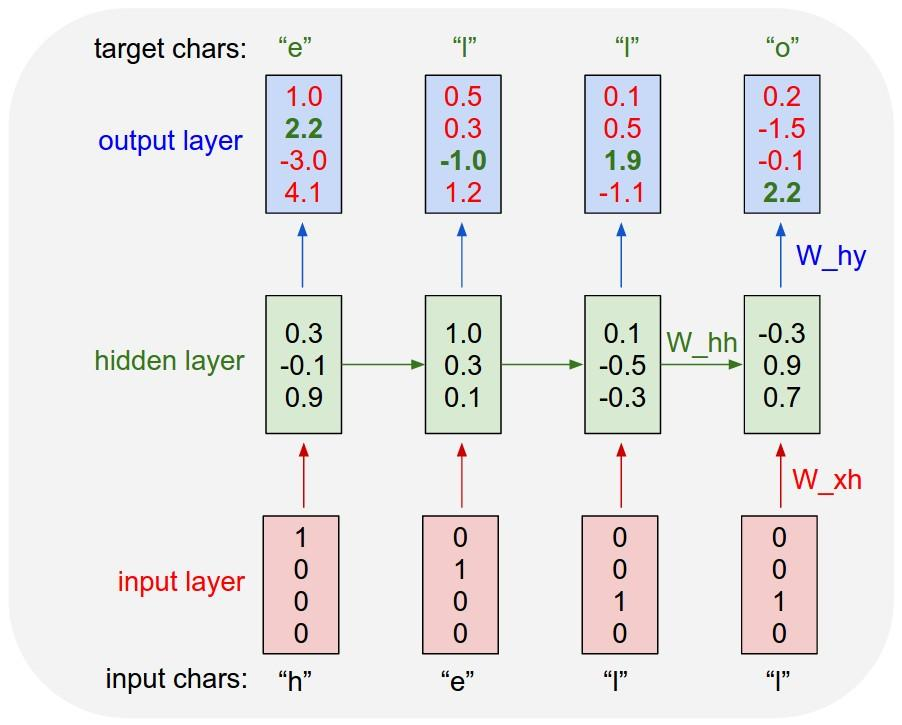
\includegraphics[width=.99\textwidth]{ak-char-rnn}  
\end{minipage}

\end{frame}



\begin{frame}
  \frametitle{Trained on Shakespeare's sonnets}
  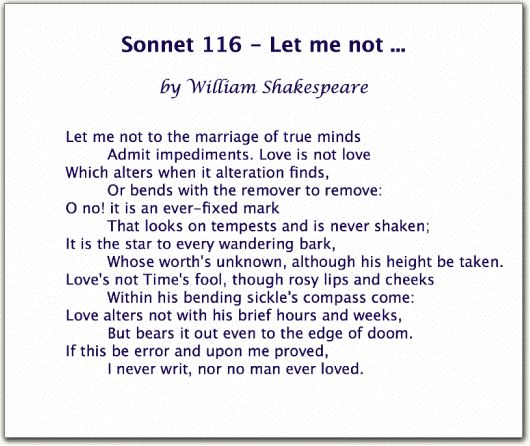
\includegraphics[width=.7\textwidth]{ak-shakespear}\\
{[A. Karpathy]}
\end{frame}

\begin{frame}
  \frametitle{Trained on algebraic topology text}
    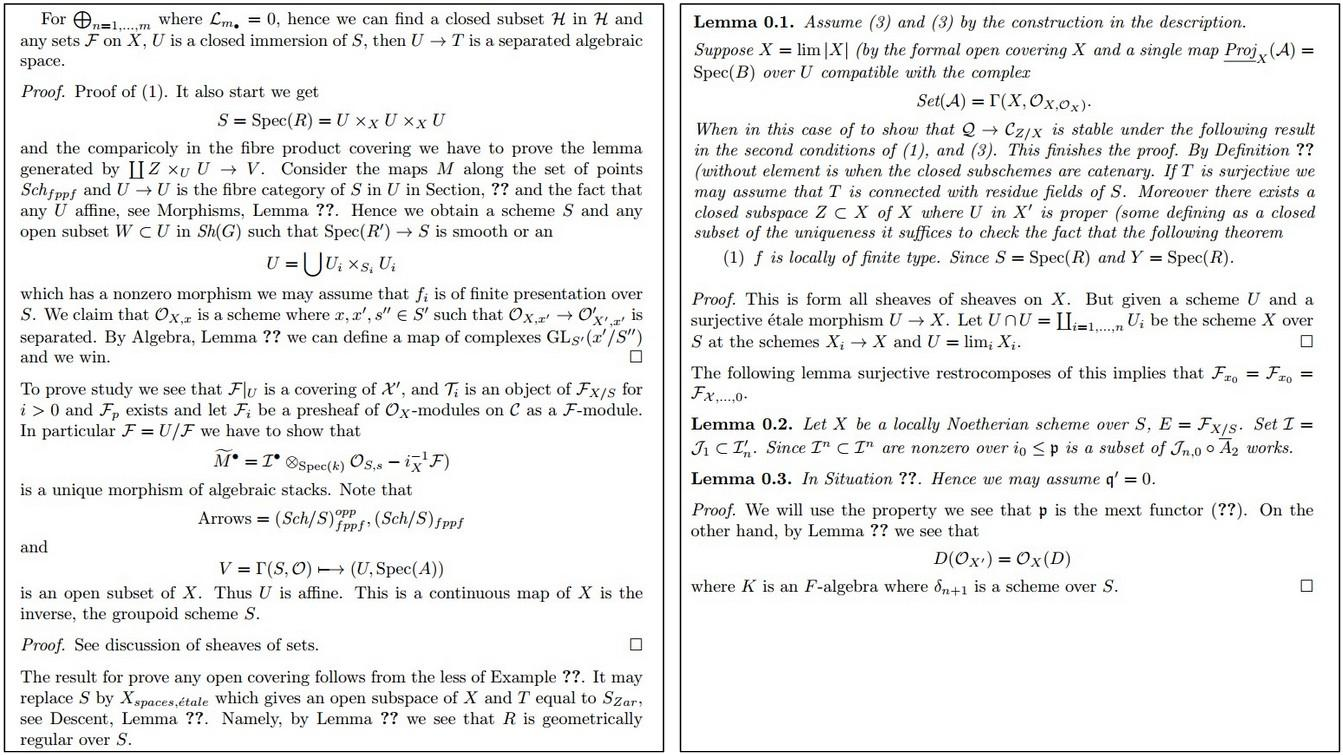
\includegraphics[width=.9\textwidth]{ak-topology}\\
{[A. Karpathy]}
\end{frame}


\begin{frame}
  \frametitle{Training one-to-many models}
  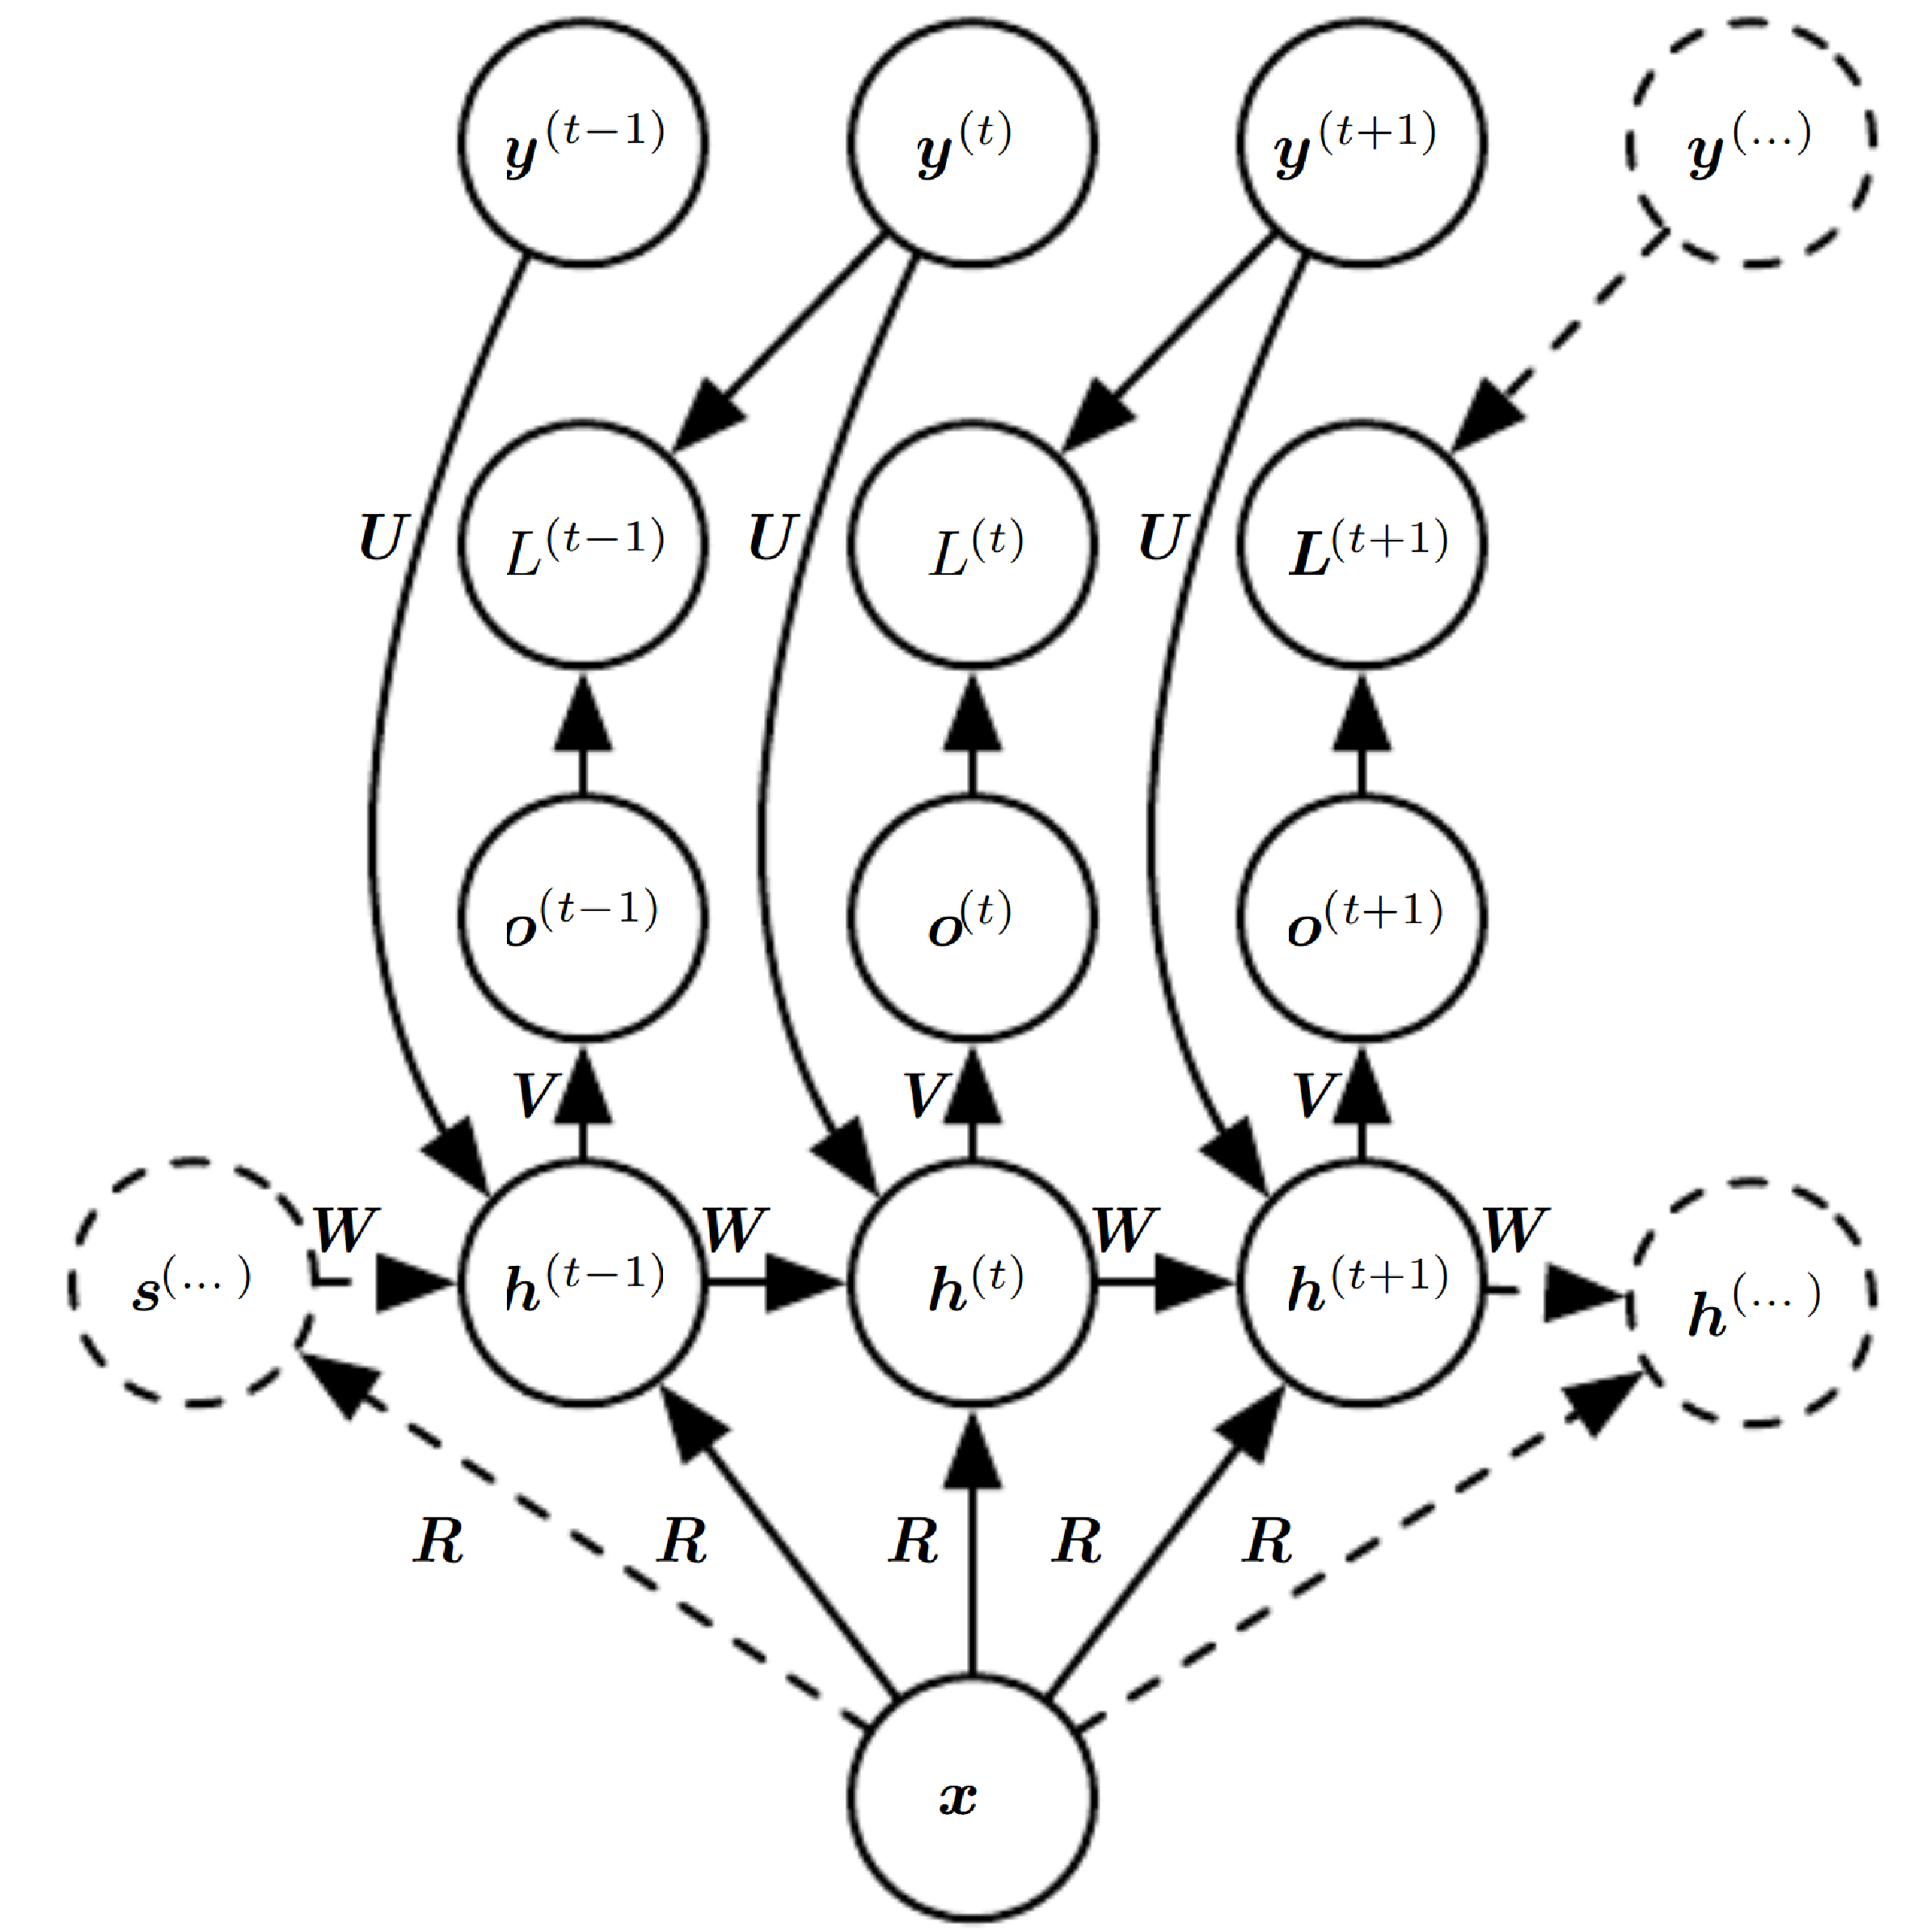
\includegraphics[width=.6\textwidth]{gcb-x2seq-varlen}\raisebox{1em}{[Goodfellow
  et al.]}
\bi
\item Loss is per frame; at training time previous true label is used (cheating?)
\ei
\end{frame}

\begin{frame}
  \frametitle{Example: image captioning model}
  \bi
\item One-to-many, e.g., image captioning: $\mathbf{i}$ is image features,
  $y_0,y_1,\ldots$ is the word sequence
\item Words are encoded as vectors $\mathbf{x}_t$ (one-hot, or an
  embedding like Word2Vec), with special {\tt START} and {\tt END} words.
\ei
\begin{minipage}[c]{.5\linewidth}
  \bi
\item Network definition:
  \begin{align*}
    \mathbf{h}_1&=g(\mathbf{W}_{ih}\mathbf{i}+\mathbf{W}_{xh}\vx(\texttt{START}))\\
    \mathbf{h}_t&=g(\mathbf{W}_{xh}\vx_t+\mathbf{W}_{hh}\mathbf{h}_{t-1})\\
    \mathbf{o}_t&=g(\mathbf{W}_{ho}\mathbf{h})\\
    y_t&=\texttt{softmax}(\mathbf{o}_t)
  \end{align*}

\ei
\end{minipage}%
\begin{minipage}[c]{.5\linewidth}
  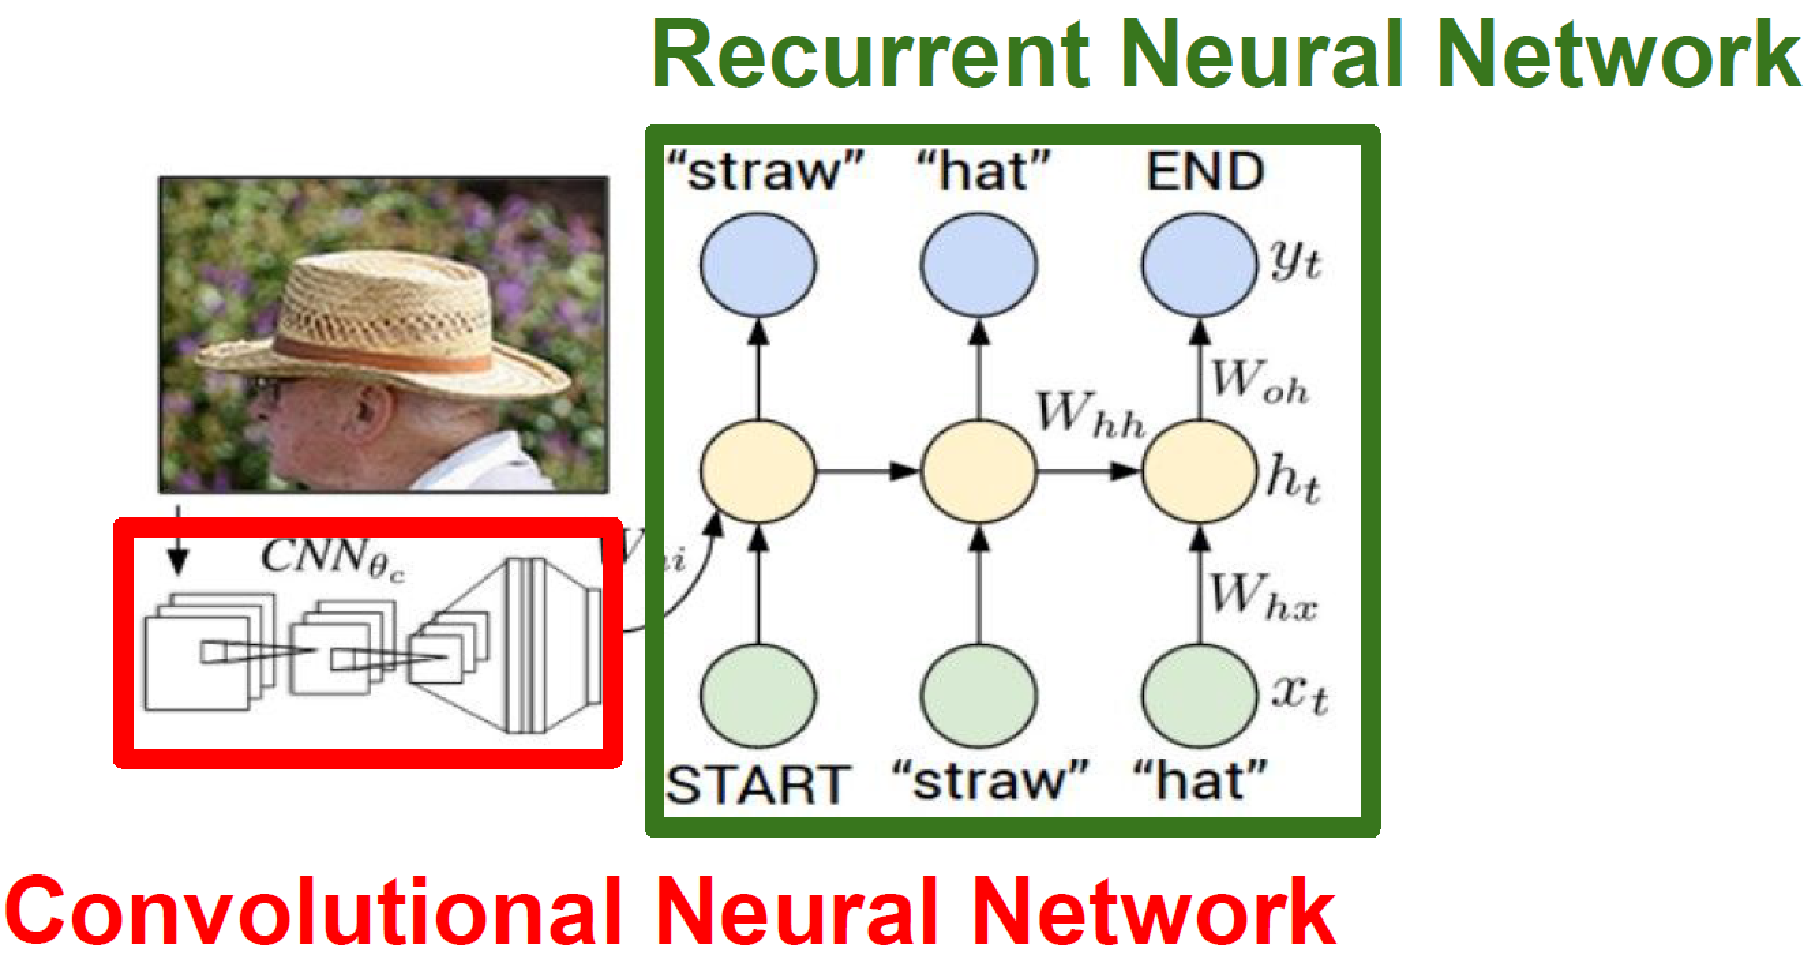
\includegraphics[width=.99\textwidth]{ak-imagecaption}
\end{minipage}

\end{frame}


\begin{frame}
  \frametitle{Image captioning: training and testing}
  \begin{minipage}[c]{.5\linewidth}
     \begin{align*}
    \mathbf{h}_1&=g(\mathbf{W}_{ih}\mathbf{i}+\mathbf{W}_{xh}\vx(\texttt{START}))\\
    \mathbf{h}_t&=g(\mathbf{W}_{xh}\vx_t+\mathbf{W}_{hh}\mathbf{h}_{t-1})\\
    \mathbf{o}_t&=g(\mathbf{W}_{ho}\mathbf{h})\\
    y_t&=\texttt{softmax}(\mathbf{o}_t)
  \end{align*}
  \end{minipage}%
  \begin{minipage}[c]{.5\linewidth}
      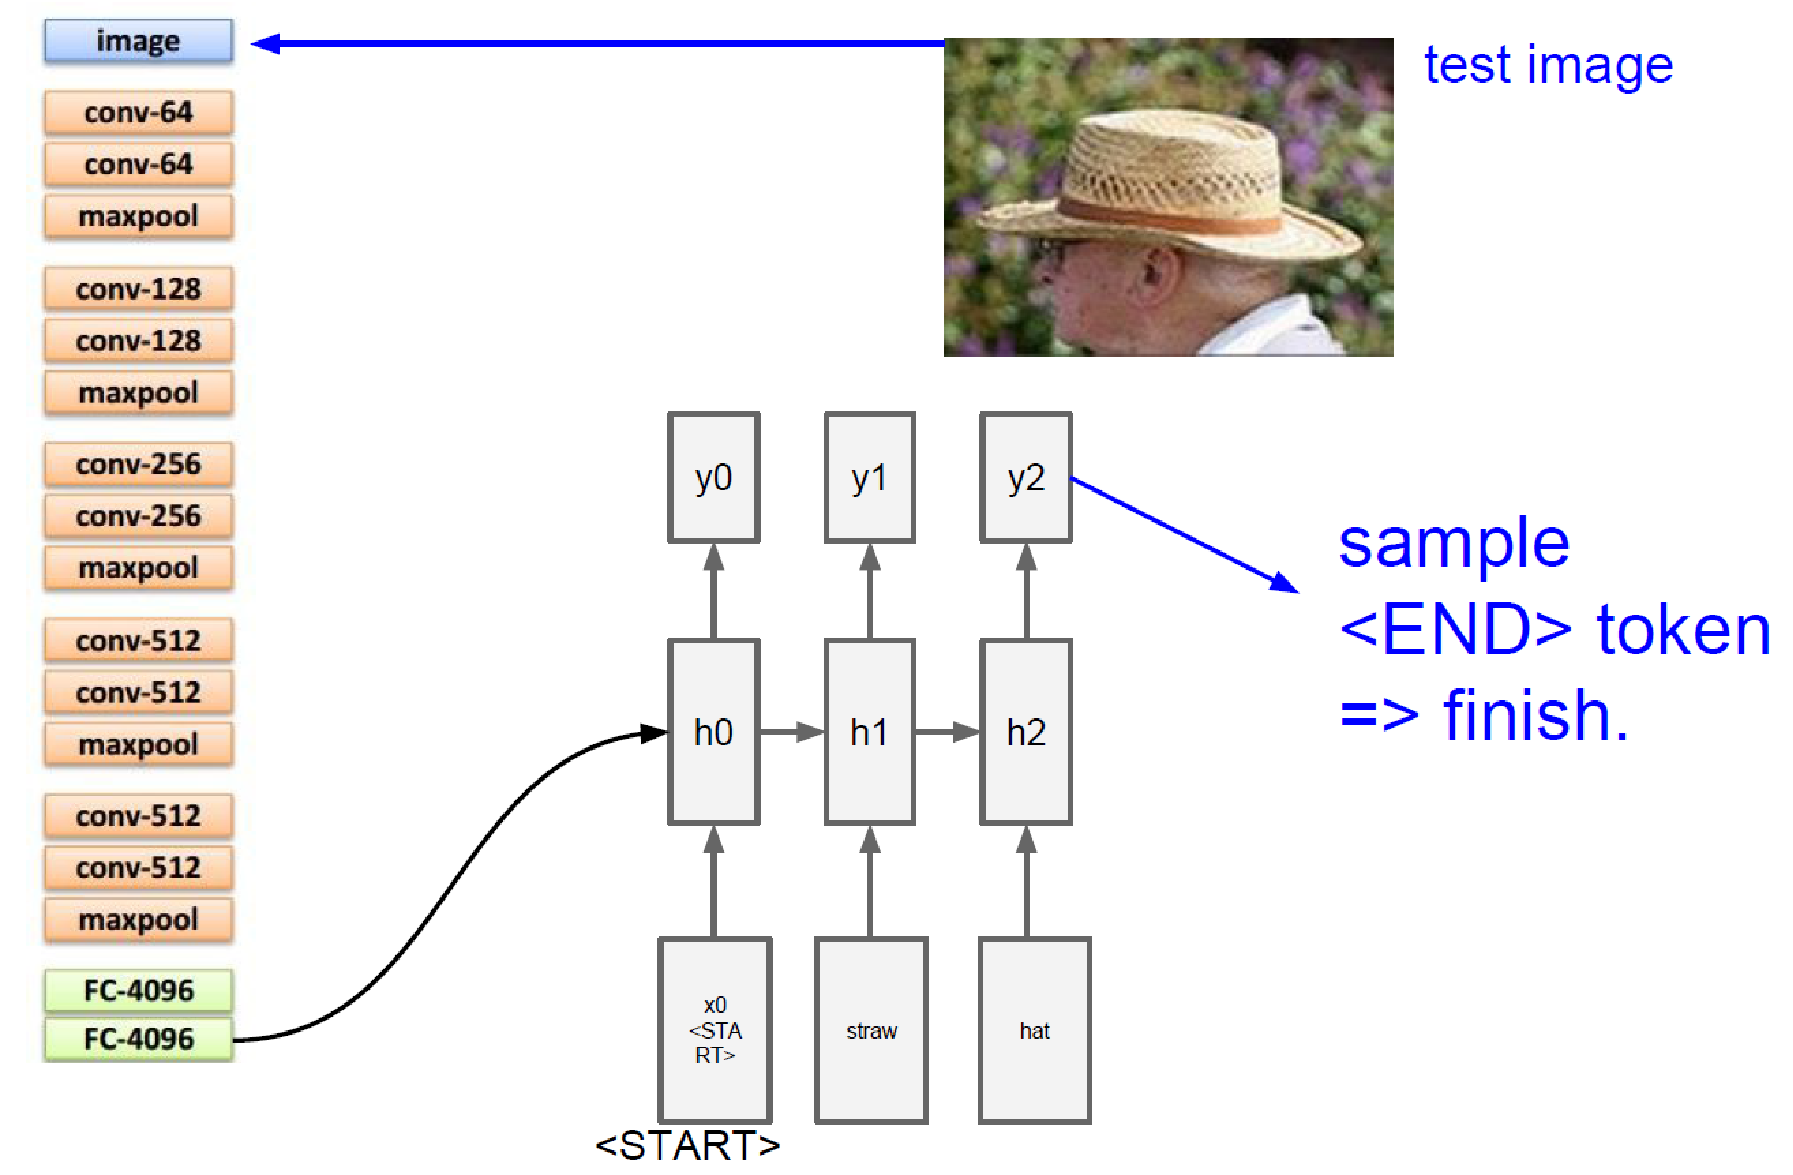
\includegraphics[width=.99\textwidth]{ak-imagecaption-run}\\
      {[A. Karpathy]}
  \end{minipage}
\bi
\item Training: $\vx_t$ is the \emph{ground truth} word (ignore
  prediction)
\item Test: $\vx_t$ is sampled from softmax distribution obtained from
  $\mathbf{o}_t$
\item Length of output sequence is determined at test time by waiting
  for {\tt END}
\item CNN for extracting $\mathbf{i}$ is initialized from ImageNet,
  can be fine-tuned jointly with the rest!
\ei
\end{frame}

\begin{frame}
  \frametitle{Backpropagation through time}
  \bi
\item Once unroll the RNN, can run backpropagation as usual\\
``backpropagation through time''
\item Enforce parameter sharing: e.g., first pretent it's a normal NN,
  compute gradients, then before updating, average across time frames.
\item All components of the model are trained end-to-end
\ei
\end{frame}




\begin{frame}
  \frametitle{Gradient flow in RNNs}
  \bi
\item Vanilla RNNs OK for short sequences
\item Consider gradient flow in BPTT:\\
multiply $W_{hh}$ by itself many times
\item Gradient explosion if largest eigenvalue is greater than 1!
\item Simple solution: gradient clipping
\[\text{if}\;\|\mathbf{g}\|>\tau,\qquad\mathbf{g}\,=\,\frac{\tau\mathbf{g}}{\|\mathbf{g}\|}
\]

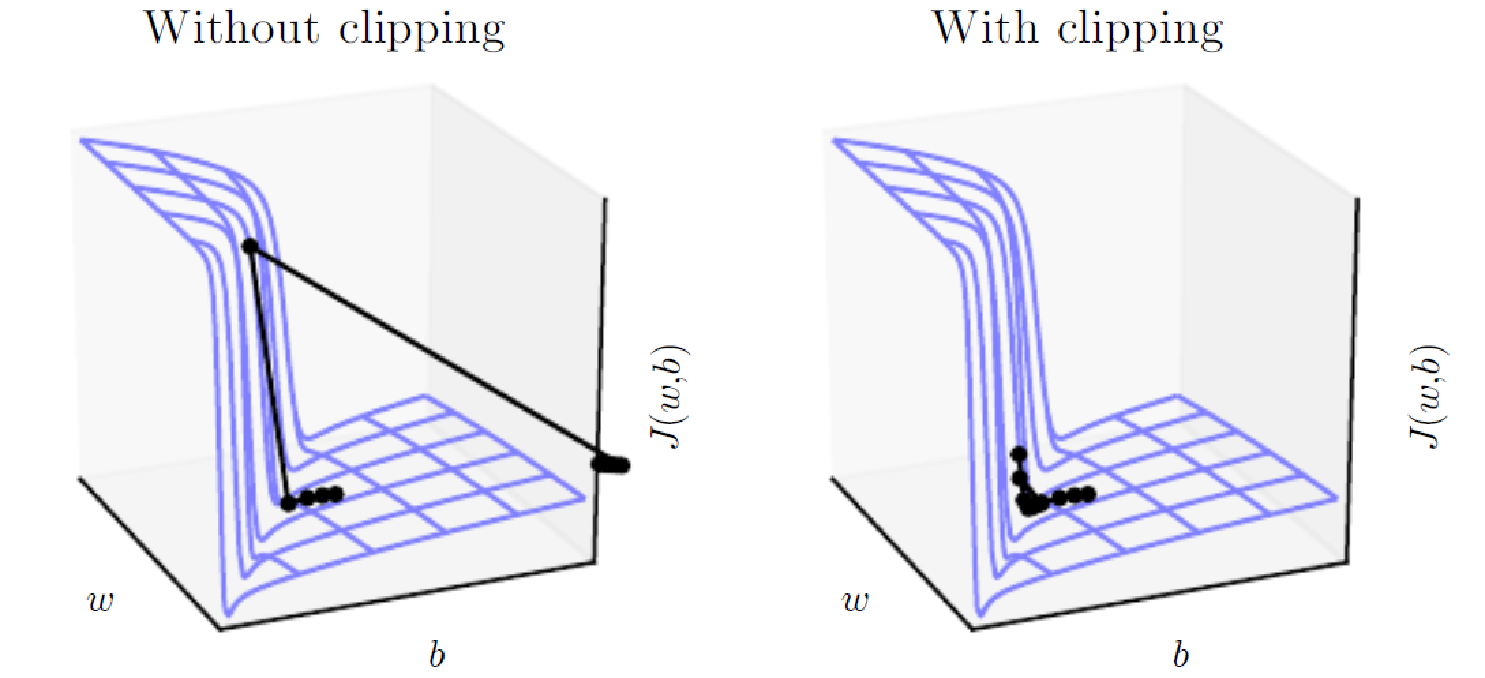
\includegraphics[width=.7\textwidth]{gcb-grad-clip}\raisebox{1em}{[Goodfellow
  et al.]}

\ei
\end{frame}

\begin{frame}
  \frametitle{Limited memory problem}
  \bi
\item When largest eigenvalue is less than 1, we can have vanishing
  gradient
\item This leads to forgetting

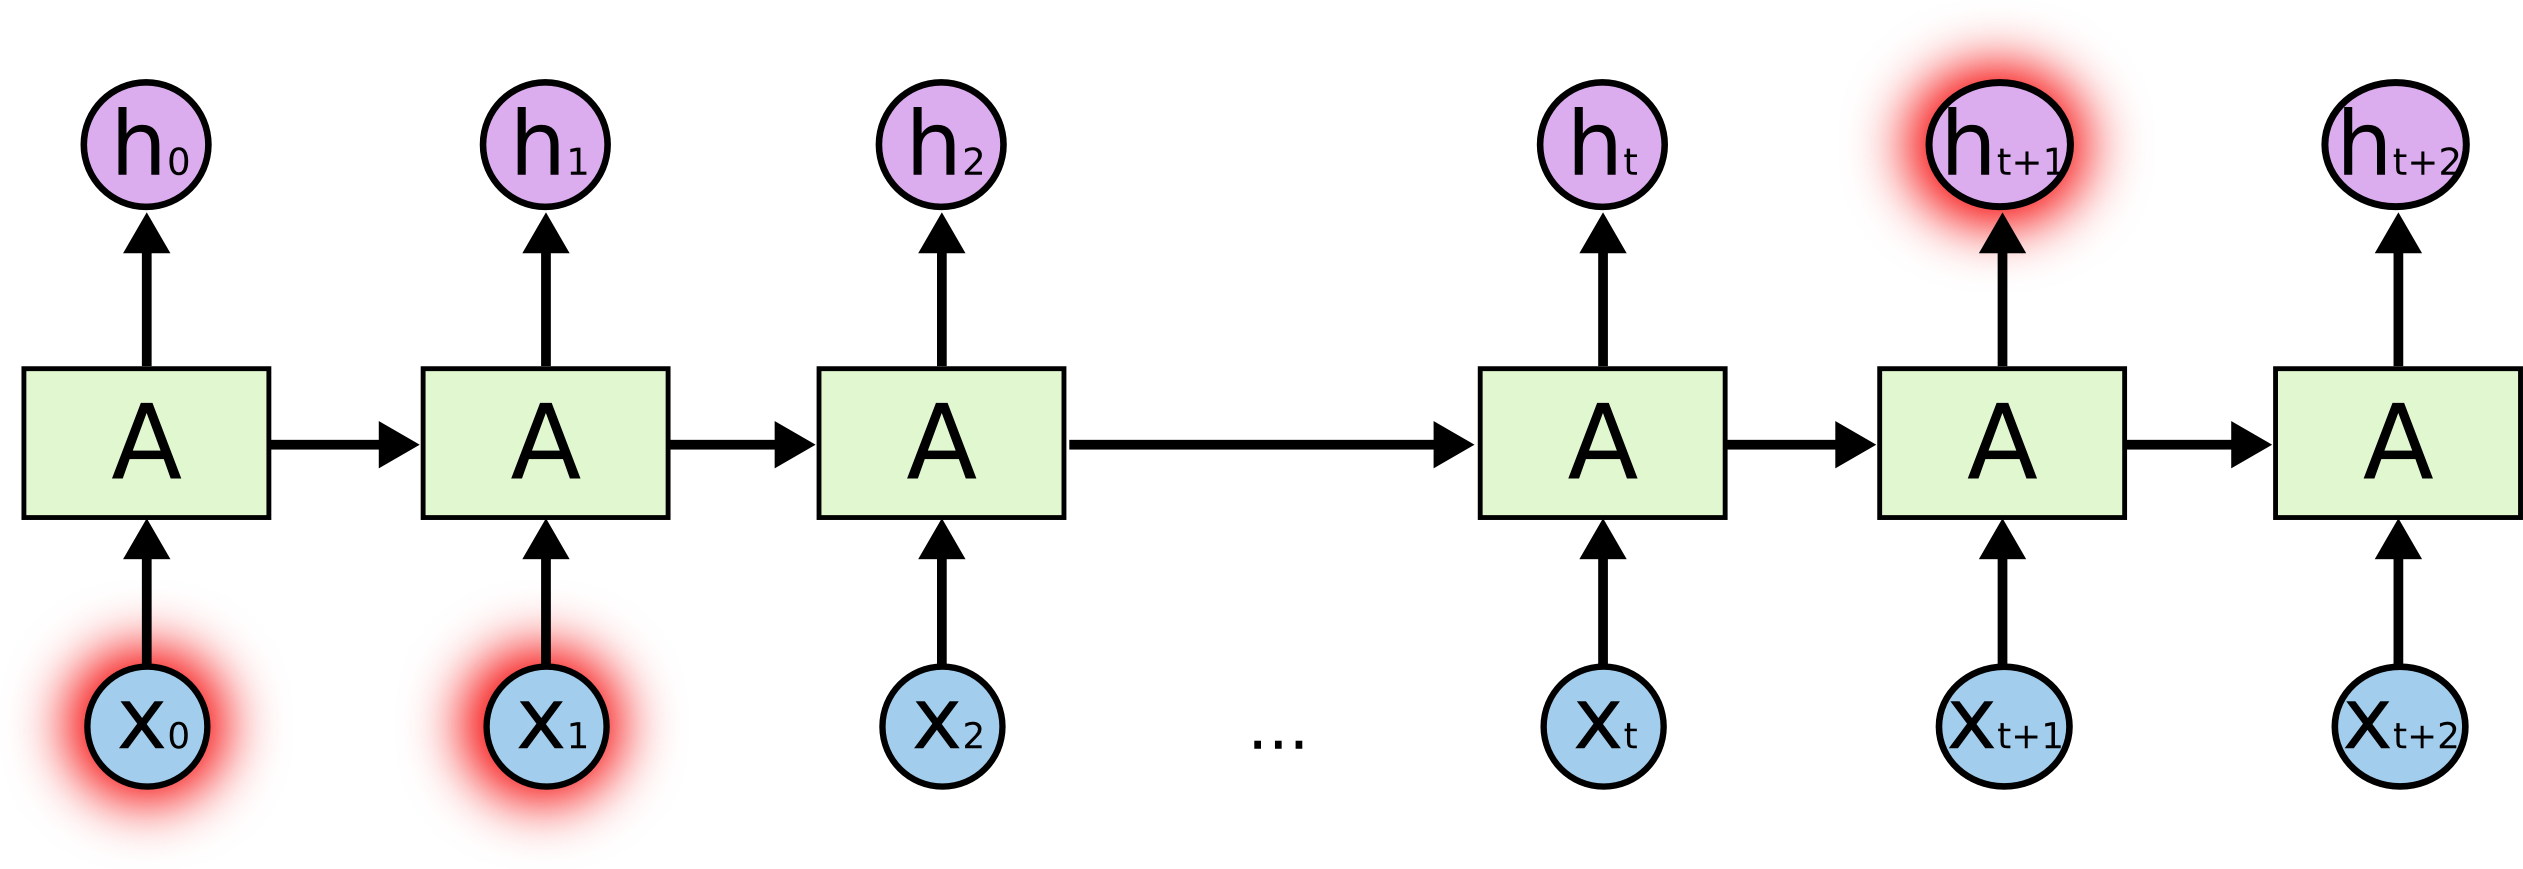
\includegraphics[width=.7\textwidth]{olah-lstm/RNN-longtermdependencies}~\raisebox{1em}{[C. Olah]}
\item Consider: ``I grew up in France, I speak fluent French''\\
or translating between languages with long-term dependencies
\ei
\end{frame}

\begin{frame}
  \frametitle{Long Short Term Memory}

\bi
  \item LSTM introduced by Hochreiter and Schmidh\"uber in 1997
\item Each time frame is associated with a complex cell

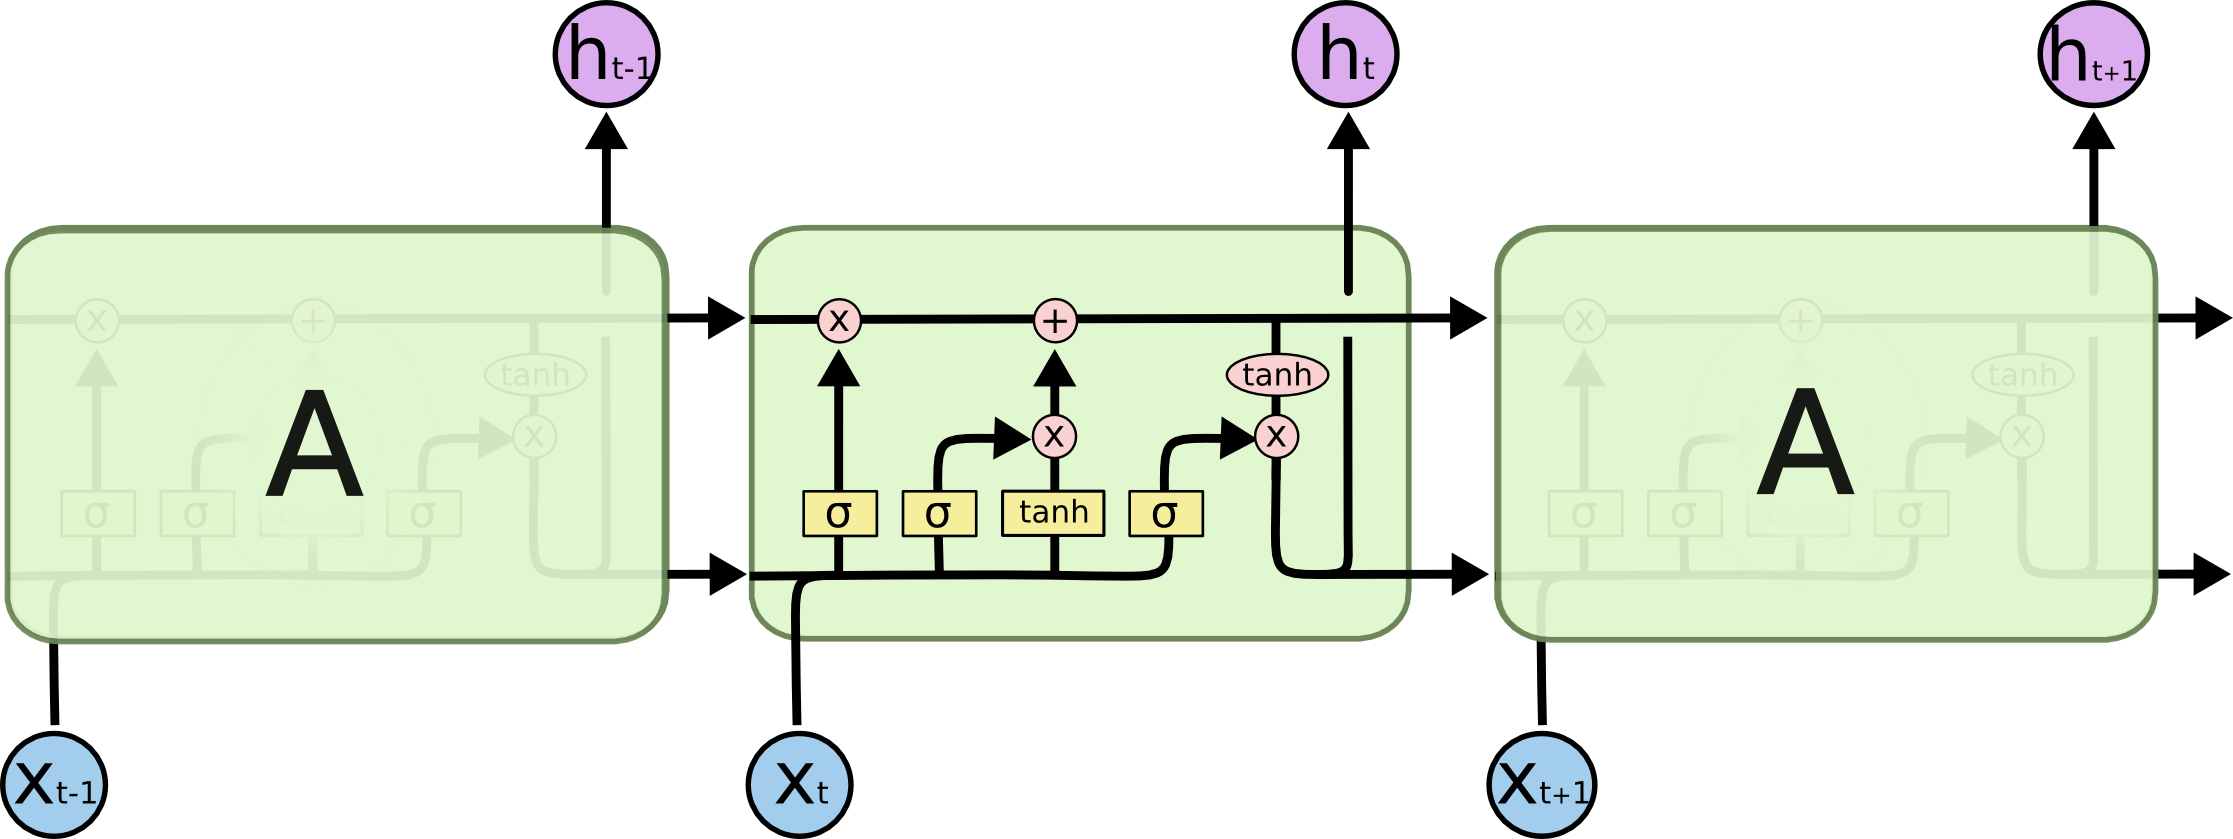
\includegraphics[width=.8\textwidth]{olah-lstm/LSTM3-chain}\\
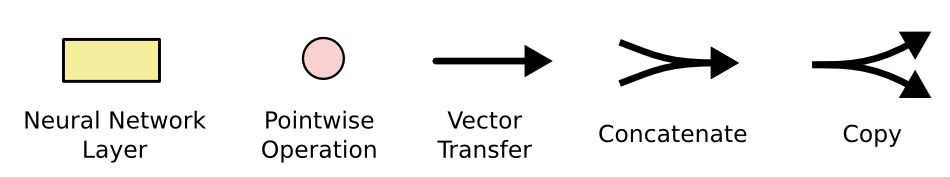
\includegraphics[width=.5\textwidth]{olah-lstm/LSTM2-notation}

\item This and subsequent LSTM figures credit: C. Olah
\ei

\end{frame}

\begin{frame}
  \frametitle{Simple RNN cells}
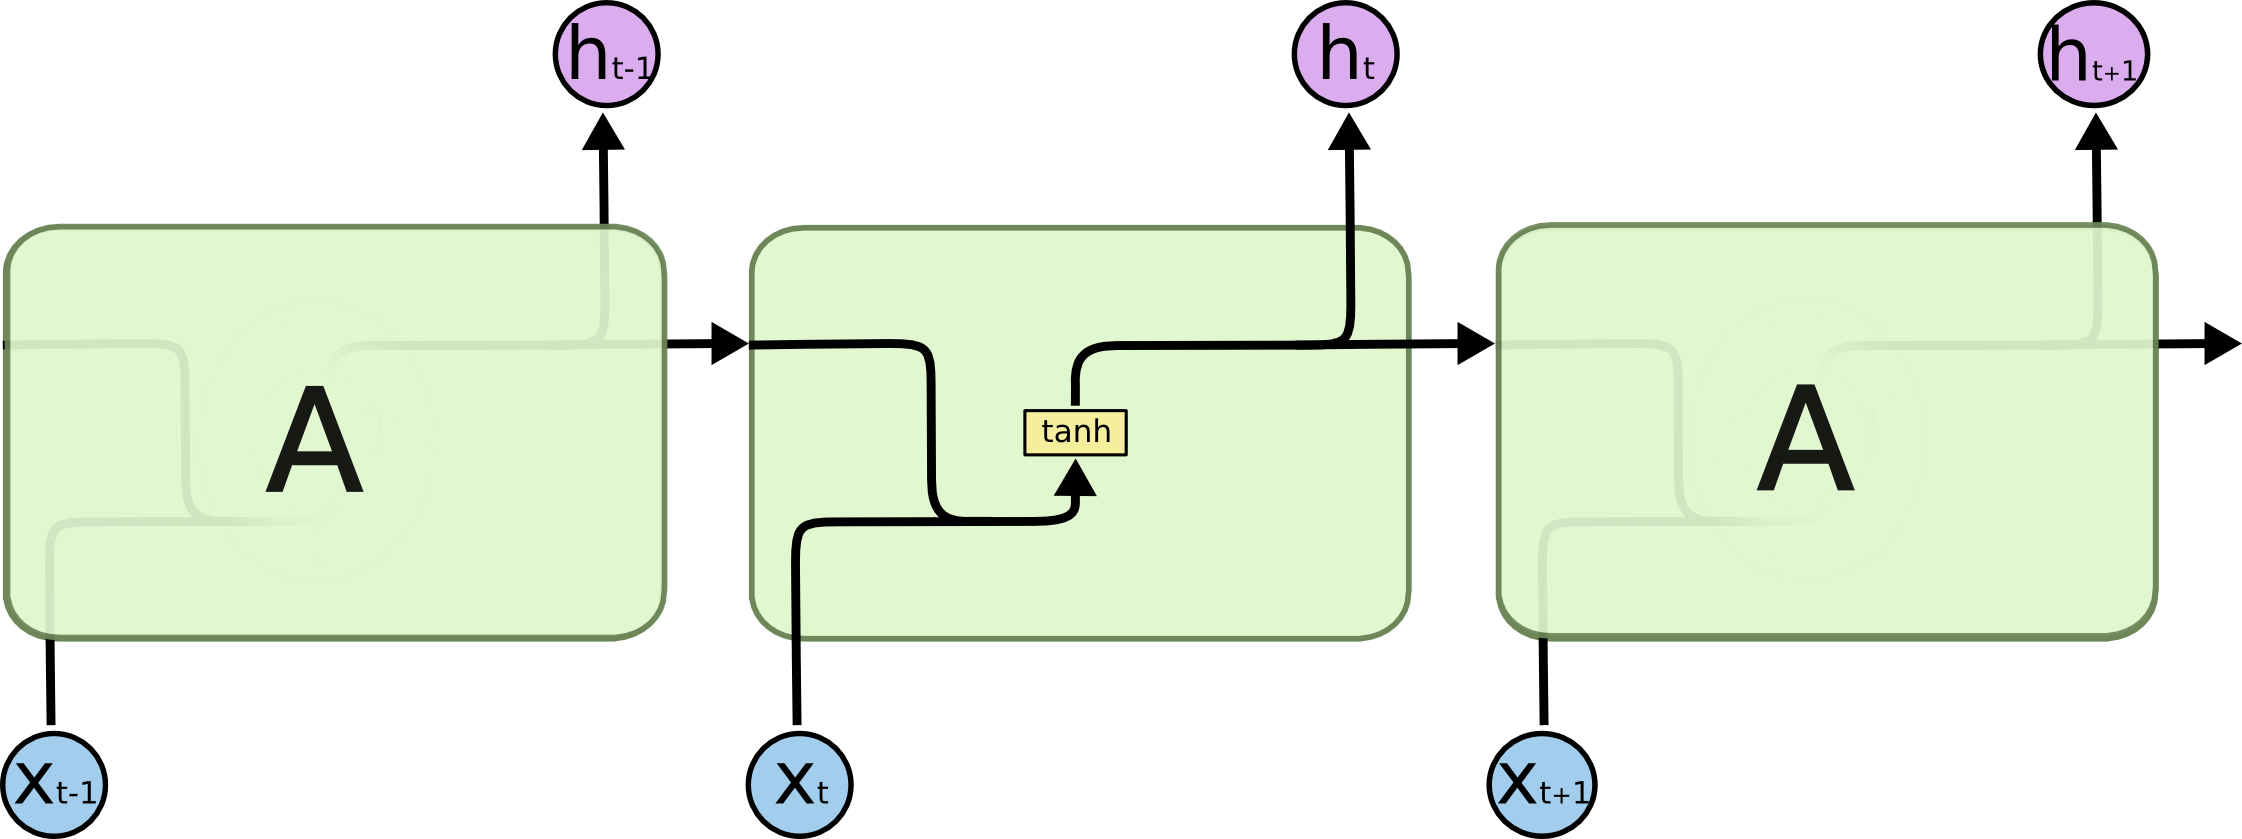
\includegraphics[width=.8\textwidth]{olah-lstm/LSTM3-SimpleRNN}\\
\includegraphics[width=.5\textwidth]{olah-lstm/LSTM2-notation}
\end{frame}


\begin{frame}
  \frametitle{LSTM:  state and gating}
  
\bi\item The core flow through LSTM cell is via the ``cell state''

\includegraphics[width=.9\textwidth]{olah-lstm/LSTM3-C-line}
\ei
\begin{minipage}[c]{.8\linewidth}
  \bi
\item Gates multiply a value by the output of a sigmoid neural network
  (possibly one layer);
\item 0 means ``block'', 1 means ``pass through''
\ei
\end{minipage}%
\begin{minipage}[c]{.2\linewidth}
  \includegraphics[width=.5\textwidth]{olah-lstm/LSTM3-gate}
\end{minipage}
\includegraphics[width=.5\textwidth]{olah-lstm/LSTM2-notation}
\end{frame}

\begin{frame}
  \frametitle{LSTM: forget gate}
  \includegraphics[width=.9\textwidth]{olah-lstm/LSTM3-focus-f}\\
\includegraphics[width=.5\textwidth]{olah-lstm/LSTM2-notation}
\bi
\item Forget gate determines whether to keep information in the hidden
  state
\item Example: gender of a subject (forget if dealing with new
  subject)
\item Note: gating is elementwise (per dimension of $\mathbf{h}$)
\ei
\end{frame}

\begin{frame}
  \frametitle{LSTM: input gate}
  \includegraphics[width=.9\textwidth]{olah-lstm/LSTM3-focus-i}\\
\includegraphics[width=.5\textwidth]{olah-lstm/LSTM2-notation}
\bi
\item Input gate: determines which values to influence by input
\item Separate layer creates ``candidate values'' $\tilde{C}_t$ to add
  to state\\
use $\tanh$ to allow for signed values\\
Note: often called $g$ in literature
\item Of $\mathbf{i}_{t,j}=0$ we will ignore $\tilde{C}_{t,j}$ (i.e.,
  will not ``form new memories'' for dimension $j$ of hidden state
  based on input in frame $t$
\ei
\end{frame}

\begin{frame}
  \frametitle{LSTM: applying updates}
   \includegraphics[width=.9\textwidth]{olah-lstm/LSTM3-focus-C}\\
\includegraphics[width=.5\textwidth]{olah-lstm/LSTM2-notation}
\bi
\item Apply the forgetting and new memory formation according to
  forget and input gate outputs and $\tilde{C}$
\ei

\end{frame}

\begin{frame}
  \frametitle{LSTM: output gate}
   \includegraphics[width=.9\textwidth]{olah-lstm/LSTM3-focus-o}\\
\includegraphics[width=.5\textwidth]{olah-lstm/LSTM2-notation}
\bi
\item Output gate $\mathbf{o}_t$ determines which dimensions of the
  state $\mathbf{C}$ will be incorporated in the output of the cell
  (i.e., in $\mathbf{h}_t$)
\item Note: use $\tanh$, so values in $[-1,1]$
\ei
\end{frame}

\begin{frame}
  \frametitle{Gated Recurrent Units}
  \bi
\item GRU [Cho et al.] is a simpler model

 \includegraphics[width=.9\textwidth]{olah-lstm/LSTM3-var-GRU}\\
\includegraphics[width=.5\textwidth]{olah-lstm/LSTM2-notation}
\item Merge forget and input gate
\item Merge cell state and hidden state
\item Since introduction in 2014 becoming more popular
\ei
\end{frame}

\begin{frame}
  \frametitle{Sequence to sequence LSTM models}
  \includegraphics[height=.7\textheight]{gcb-rnn-encdec}\raisebox{1em}{[Goodfellow
  et al.]}
\bi
\item Encoder-decoder: first RNN encodes input, captures context in
  $C$;\\second RNN decodes
  output
\item First competitive neural MT model [Sutskever et
  al., 2014]
\ei
\end{frame}

\begin{frame}
  \frametitle{Deep RNNs}
  \bi
\item Straightforward to add layers to $\mathbf{h}$
\includegraphics[width=.5\textwidth]{ak-deep-rnn}\raisebox{1em}{[A. Karpathy]}
\ei
\end{frame}


\end{document}
